%%==================================================
%% diss.tex for SJTU Master Thesis
%% based on CASthesis
%% modified by wei.jianwen@gmail.com
%% version: 0.3a
%% Encoding: UTF-8
%% last update: Dec 5th, 2010
%%==================================================

% 字号选项: c5size 五号(默认) cs4size 小四
% 双面打印(注意字号设置)
\documentclass[cs4size, a4paper, twoside]{sjtumaster-xetex}
% 单面打印(注意字号设置)
% \documentclass[cs4size, a4paer, oneside, openany]{sjtumaster-xetex}


% \usepackage[sectionbib]{chapterbib}%每章都用参考文献

\newboolean{DOIT}
\setboolean{DOIT}{false}%编译某些只想自己看的内容,编译true,否则false

%% 行距缩放因子(x倍字号)
\renewcommand{\baselinestretch}{1.3}

% 设置图形文件的搜索路径
\graphicspath{{figure/}{figures/}{logo/}{logos/}{graph/}{graphs}}

%%========================================
%% 在sjtumaster-xetex.cls中定义的有用命令
%%========================================
% \cndash 中文破折号
% 数学常量
% \me 对数常数e
% \mi 虚数单位i
% \mj 虚数单位j
% \dif 直立的微分算符d为直立体。
% 可伸长的数学箭头、等号
% \myRightarrow{}{}
% \myLeftarrow{}{}
% \myBioarrow{}{}
% \myLongEqual{}{}
% 参考文献
% \upcite{} 上标引用
%%========================================

\begin{document}

%%%%%%%%%%%%%%%%%%%%%%%%%%%%%%
%% 封面
%%%%%%%%%%%%%%%%%%%%%%%%%%%%%%

% 中文封面内容(关注内容而不是形式)
\title{移动网络通信质量测试、建模与系统实现}
\author{马~永森}
\advisor{龙~承念\quad{}教授}
\degree{硕士}
\defenddate{2013年1月16日}
\school{上海交通大学}
\institute{自动化系}
\studentnumber{1100329074}
\major{控制科学与工程}

%\title{移动网络通信质量测试、建模与系统实现}
%\author{XXX}
%\advisor{XXX}
%\degree{硕士}
%\defenddate{XXXX.XX.XX}
%\school{上海交通大学}
%\institute{自动化系}
%\studentnumber{XXX}
%\major{控制科学与工程}

% 英文封面内容(关注内容而不是表现形式)
\englishtitle{Performance Measurement and Modeling in Mobile Wireless Networks}
\englishauthor{\textsc{Yongsen MA}}
\englishadvisor{Prof. \textsc{Chengnian Long}}
\englishschool{Shanghai Jiao Tong University}
\englishinstitute{\textsc{Depart of Automation} \\ \textsc{School of Electronic, Information and Electrical Engineering} \\
  \textsc{Shanghai Jiao Tong University} \\
  \textsc{Shanghai, P.R.China}}
\englishdegree{Master}
\englishmajor{Control Science and Engineering}
\englishdate{Jan. 16th, 2013}

%\englishtitle{Performance Measurement and Modeling in Mobile Wireless Networks}
%\englishauthor{XXX}
%\englishadvisor{XXX}
%\englishschool{Shanghai Jiao Tong University}
%\englishinstitute{\textsc{Depart of Automation} \\ \textsc{School of Electronic, Information and Electrical Engineering} \\
%  \textsc{Shanghai Jiao Tong University} \\
%  \textsc{Shanghai, P.R.China}}
%\englishdegree{Master}
%\englishmajor{Control Science and Engineering}
%\englishdate{XXXX.XX.XX}

% 封面
\maketitle

% 英文封面
\makeenglishtitle

% 论文原创性声明和使用授权
%\makeDeclareOriginal
%\makeDeclareAuthorization

%%%%%%%%%%%%%%%%%%%%%%%%%%%%%%
%% 前言
%%%%%%%%%%%%%%%%%%%%%%%%%%%%%%
\frontmatter

% 摘要
%%==================================================
%% abstract.tex for SJTU Master Thesis
%% based on CASthesis
%% modified by wei.jianwen@gmail.com
%% version: 0.3a
%% Encoding: UTF-8
%% last update: Dec 5th, 2010
%%==================================================

\begin{abstract}

近年来,无线网络尤其是移动网络发展迅速,一方面造成业务流量和用户需求的增加,另一方面带来频谱利用率的下降,因此如何通过有效的资源分配实现系统可靠性与网络传输性能的平衡成为移动网络的关键问题。传统的频谱资源分配一般采用理论上的无线传播或链路质量模型,但是这些模型由于忽略了多径效应和移动性等因素,在实际应用过程中通常难以实现有效的资源调度与分配。实际应用中一般利用实测数据对当前网络状态进行评估,同时实现无线资源的动态分配,如功率控制、速率适配及接入控制等,因此实时准确的通信质量测试对于移动网络的可靠稳定运行至关重要。移动无线网络通信质量最重要的两项指标为信道状态与链路质量,分别表征了其物理层与链路层的通信质量信息,同时也是网络运行与优化的重要参数,因此两者的准确高效的测量能实现移动网络可靠性与传输性能的有效平衡。对于移动无线网络通信质量测试而言,主要问题是如何在不同的网络场景与系统需求下,实现测试精度与开销之间的有效平衡。

首先,由于GSM-R网络对安全性具有严格要求,现有测试方法均采用高频采样,成本较高且仅适用于离线测试,无法应用于在线测试及资源调度。对于高速移动网络GSM-R而言,在满足测量精度的前提先应尽量降低其测试开销,实现对GSM-R网络的在线实时测试,保证整个高铁系统的稳定可靠运行。而GSM-R网络具有移动终端高速移动性和无线传播环境复杂性的特点,从而对其通信质量测试形成巨大挑战。传统的信号强度测试算法无法直接应用于GSM-R网络测试中,这就要求GSM-R网络信号强度测试算法必须具有实时高效的特点,以适应高速铁路的特殊要求,即在高速移动条件下满足信道状态测试精度并降低测试开销。

其次,对于802.11n网络而言,除了移动性及无线传播环境的影响外,MIMO-OFDM技术进一步增加了链路质量测试与建模的复杂度。MIMO-OFDM技术一方面显著地提升了网络性能,另一方面给802.11n网络链路质量测试与建模带来新的问题:获得所有配置下的链路质量模型需要进行更多的探测与采样,同时MIMO-OFDM配置造成链路质量模型的过渡窗口效应,从而严重降低链路质量预测精度。因此如何针对802.11n网络的移动性与多配置性,设计动态的链路质量测试与建模算法,以准确刻画MIMO-OFDM配置的链路质量,从而根据当前网络状态进一步提升其网络性能,即在MIMO-OFDM多配置情况下实现不同配置链路质量模型的在线实时测试与建模。

本文主要针对高速移动网络和无线局域网络中的信道估计与链路测试问题,对移动网络的通信质量测试进行详细分析,针对高速移动特性及MIMO-OFDM多配置特性分别提出信道状态动态测试算法及链路质量在线测试与建模框架,通过当前网络状态实时调整测试参数,在满足测试精度的前提下降低测试开销,最后通过算法设计、系统实现与实验测试对移动网络通信质量测试算法进行性能评估。


  \keywords{移动无线网络,通信质量测试,GSM-R,802.11n,MIMO-OFDM,信道状态估计,链路质量建模}
\end{abstract}

\begin{englishabstract}

The mobile wireless networks have experienced rapid development in recent years, and the growth is expected to continue unabated. For different types of mobile networks, a basic consideration is the accurate channel state estimation and link quality measurement to get efficient trade-off between reliability and data rate. For GSM-R networks deployed for communications between train and railway regulation control centers in high-speed railway, it requires real-time measurement to ensure the reliability of the system \cite{baldini2010early}. At the same time, it is necessary to make dynamic measurement due to the complexity of the radio propagation environments and the varied terrains along the high-speed railway route. On the other hand, the continued success of mobile 802.11n depends on their ability to efficiently configure different PHY/MAC enhancements. This is challenging in that multi-configuration in mobile 802.11n not only requires far more samples to acquire sufficient information for all possible channel settings, but also introduces significant complications in channel modeling. Furthermore, channels are more vulnerable to environmental variability and terminal mobility in mobile 802.11n. Therefore, accurate channel measurement and prediction is becoming increasingly important in mobile wireless networks, and it is crucial to lower the estimation overhead to address the issues of mobility and multi-configuration so that real-time measurement can be implemented to ensure the reliability or data rate.

For the channel state estimation in mobile networks, Lee's method proposed a standard procedure of local average power estimation, which determined the proper length and required sampling numbers for estimating the local average in the case of Rayleigh fading channels \cite{lee1985estimate}. Velocity adaptive handoff algorithms \cite{Austin1994} get the amount of spatial averaging required for local mean estimation of Rician fading according to Lee's standard procedure by approximation, but it has too high overhead to be applied in real-time measurement. The Generalized Lee method \cite{Vega2009} allows estimating the mean values without the requirement of a priori knowing the distribution function, which is based on measured field data samples, but the optimum length of averaging interval is calculated using all the routes of the database with high overhead. This paper combines Lee's method and EM algorithm to estimate the Rician fading channels in GSM-R networks. The basic procedure is same to the Lee's method of local mean power estimation, except that the multi-path fading is Rician distributed. This method takes advantage of the sampling signals and Rician fading parameters of last estimation to improve estimation accuracy and reduce measurement overhead. The determination of proper length of statistical interval and required number of averaging samples are adaptive to different propagation environments.

Furthermore, recent studies show that Received Signal Strength (RSS) is a weak indicator for 802.11n channel quality due to the large transition window with respect to Packet Delivery Ratio (PDR), and there exists a fundamental and inevitable tradeoff between the accuracy and overhead in channel measurement and prediction. This is further complicated by the distinctive features in mobile 802.11n networks, specifically, multiple PHY/MAC settings and spatial-temporal variation channels. In this work, we present an on-line PDR-RSS modeling framework for mobile 802.11n networks. It incorporates a novel design by exploiting both packet-level and physical-level metrics, along with the diversity property of multi-configuration simultaneously to overcome channel capturing problem in the existing PDR-RSS models. This on-line framework also strikes a balance between the measurement overhead and accuracy. We further develop a rate adaption algorithm to advocate the advantage of on-line PDR-RSS modeling framework. It adopts an on-line rate selection process with high precision. Through a real world implementation on our testbed, we evaluate the proposed rate adaption algorithm over different scenarios and routes. The experimental results indicate that it can achieve throughput gains up to 40\% over the Minstrel rate control algorithm under different MIMO configurations.

  \englishkeywords{Mobile wireless network, performance measurement, GSM-R, 802.11n, MIMO-OFDM, local mean power estimation, packet delivery modeling}
\end{englishabstract}


% 目录
\tableofcontents
% 表格索引
\listoftables
% 插图索引
\listoffigures

\addcontentsline{toc}{chapter}{\listfigurename} %将表格索引加入全文目录
\addcontentsline{toc}{chapter}{\listtablename}  %将图索引加入全文目录

% 主要符号、缩略词对照表
%%==================================================
%% symbol.tex for SJTU Master Thesis
%% based on CASthesis
%% modified by wei.jianwen@gmail.com
%% version: 0.3a
%% Encoding: UTF-8
%% last update: Dec 5th, 2010
%%==================================================

\chapter{主要符号对照表}
\label{chap:symb}

\noindent
%\setlength{\parindent}{-0.5em}
\begin{supertabular}{lll}
%\begin{longtable}{lll}
GSM         & \hspace{0.5em}Global System for Mobile communications   & \hspace{0.5em}全球移动通信系统 \\
GSM-R       & \hspace{0.5em}GSM for Railways                          & \hspace{0.5em}铁路移动通信系统 \\
ITU         & \hspace{0.5em}International Telecommunication Union     & \hspace{0.5em}国际电信联盟 \\
WLAN        & \hspace{0.5em}Wireless Local Area Networks              & \hspace{0.5em}无线局域网络 \\
Wi-Fi       & \hspace{0.5em}Wireless Fidelity                         & \hspace{0.5em}无线保真 \\
%WiMAX       & \hspace{0.5em}Worldwide Interoperability for Microwave Access & \hspace{0.5em}全球微波接入互操作性 \\
MIMO        & \hspace{0.5em}Multiple-Input Multiple-Output            & \hspace{0.5em}多天线系统 \\
OFDM        & \hspace{0.5em}Orthogonal Frequency Division Multiplexing& \hspace{0.5em}正交频分复用 \\
RSS         & \hspace{0.5em}Received Signal Strength                  & \hspace{0.5em}接收信号强度 \\
SNR         & \hspace{0.5em}Signal to Noise Ratio                     & \hspace{0.5em}信噪比 \\
SINR        & \hspace{0.5em}Signal to Interference plus Noise Ratio   & \hspace{0.5em}信号与干扰加噪声比 \\
CSI         & \hspace{0.5em}Channel State Information                 & \hspace{0.5em}信道状态信息 \\
PDR         & \hspace{0.5em}Packet Delivery Ratio                     & \hspace{0.5em}数据包传输成功率 \\
QoS         & \hspace{0.5em}Quality of Service                        & \hspace{0.5em}服务质量 \\
GPS         & \hspace{0.5em}Global Positioning System                 & \hspace{0.5em}全球定位系统 \\
GIS         & \hspace{0.5em}Geographic Information System             & \hspace{0.5em}地理信息系统 \\
BS          & \hspace{0.5em}Base Station                              & \hspace{0.5em}基站 \\
MS          & \hspace{0.5em}Mobile Station                            & \hspace{0.5em}移动台 \\
AP          & \hspace{0.5em}Access Point                              & \hspace{0.5em}接入点 \\
EWMA        & \hspace{0.5em}Exponentially Weighted Moving Average     & \hspace{0.5em}指数加权移动平均 \\
DWSA        & \hspace{0.5em}Dynamic Weighted Sliding Average          & \hspace{0.5em}动态加权滑动平均 \\
MCS         & \hspace{0.5em}Modulation and Coding Scheme              & \hspace{0.5em}调制与编码策略 \\
MAC         & \hspace{0.5em}Medium Access Control                     & \hspace{0.5em}媒介访问控制 \\
SDM         & \hspace{0.5em}Spatial Division Multiplexing             & \hspace{0.5em}空分复用 \\
MSDU        & \hspace{0.5em}MAC Service Data Units                    & \hspace{0.5em}服务数据单元 \\
MPDU        & \hspace{0.5em}MAC Protocol Data Units                   & \hspace{0.5em}协议数据单元 \\
A-MSDU      & \hspace{0.5em}Aggregation of MSDU                       & \hspace{0.5em}聚合服务数据单元 \\
A-MPDU      & \hspace{0.5em}Aggregation of MSDU                       & \hspace{0.5em}聚合协议数据单元 \\
STBC        & \hspace{0.5em}Space Time Block Coding                   & \hspace{0.5em}空时编码 \\
GI          & \hspace{0.5em}Guard Interval                            & \hspace{0.5em}保护时隙 \\
LGI         & \hspace{0.5em}Long Guard Interval                       & \hspace{0.5em}长保护时隙 \\
SGI         & \hspace{0.5em}Short Guard Interval                      & \hspace{0.5em}短保护时隙 \\
ACK         & \hspace{0.5em}Acknowledgement                           & \hspace{0.5em}应答 \\
MLE         & \hspace{0.5em}Maximum Likelihood Estimation             & \hspace{0.5em}最大似然估计 \\
MMSE        & \hspace{0.5em}Minimum Mean Square Error                 & \hspace{0.5em}最小均方误差 \\
XML         & \hspace{0.5em}eXtensible Markup Language                & \hspace{0.5em}可扩展标记语言 \\
%\end{longtable}
\end{supertabular}
%\setlength{\parindent}{2em}


%%%%%%%%%%%%%%%%%%%%%%%%%%%%%%
%% 正文
%%%%%%%%%%%%%%%%%%%%%%%%%%%%%%
\mainmatter


%% 各章正文内容
%%==================================================
%% chapter01.tex for SJTU Master Thesis
%% based on CASthesis
%% modified by wei.jianwen@gmail.com
%% version: 0.3a
%% Encoding: UTF-8
%% last update: Dec 5th, 2010
%%==================================================

%\bibliographystyle{sjtu2} %[此处用于每章都生产参考文献]
\chapter{背景介绍}
\label{chap:background}

移动无线网络中的一个基本问题是如何在系统可靠性与网络传输性能之间进行有效平衡,对于高速移动网络而言,首先要保证其系统可靠性以实现信息的可靠传输;而无线局域网络则更关注网络的传输性能,包括网络吞吐量及覆盖范围等。其中信道状态和链路质量作为无线网络可靠性与传输性能的衡量指标,同时也是网络运行与优化的重要参数,因此两者的准确高效的测量对于移动网络中可靠性与传输性能的有效平衡至关重要。本文主要针对高速移动网络和无线局域网络中的信道估计与链路测试问题,对移动网络的通信质量测试进行详细分析,并通过算法设计、系统实现与实验测试对移动网络通信质量测试算法进行性能评估。

\section{移动无线网络}
\label{sec:mobile}


\subsection{高速移动网络}
\label{sec:gsmr}

在高速铁路的快速发展的过程中,列车的安全稳定运行至关重要,要实现高铁的安全稳定高速运行,必须实时地对整个高铁系统进行安全监测。其中列控系统保证高铁系统的可靠运行,GSM-R无线网络则是列控系统中的关键环节,同时又是系统中最脆弱的部分。GSM-R网络是专门应用于铁路环境中的综合数字调度移动通信网络,如图 \ref{fig:gsmrservice} 所示,GSM-R网络承载了高速铁路的列车运行状态数据传输、列车控制数据传输、区间移动公务通信、应急指挥通信等业务,因此对GSM-R网络进行实时监测具有重要意义。

\begin{figure}[!htp]
\centering
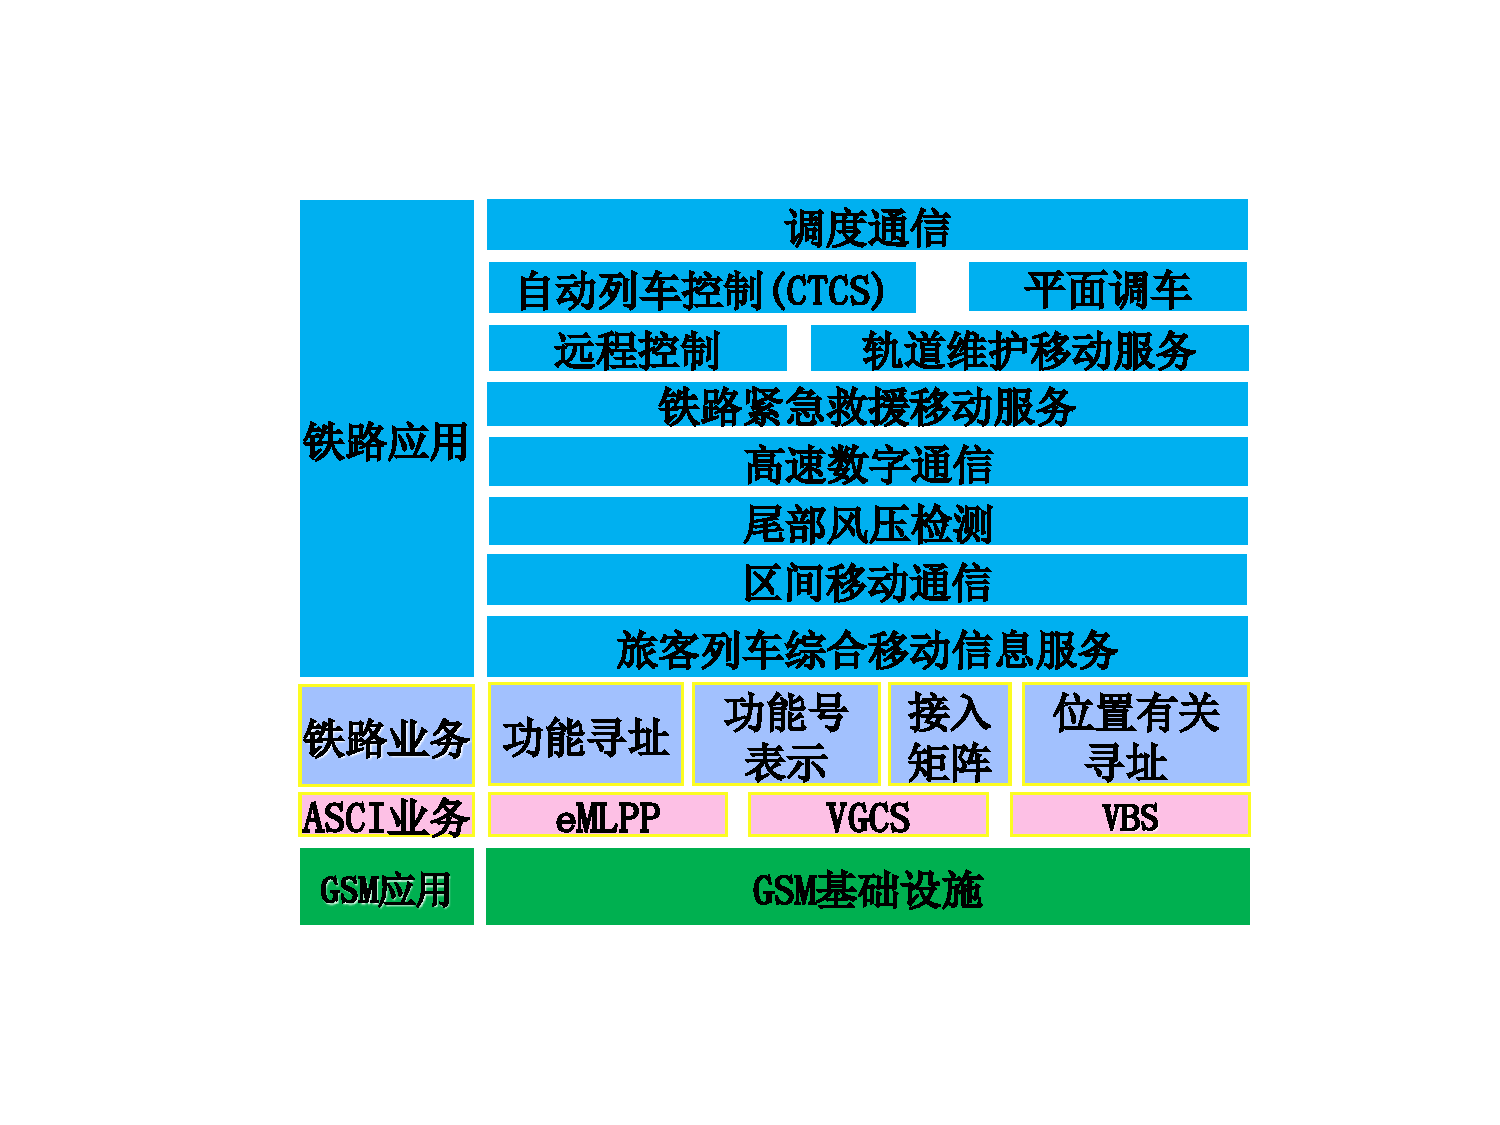
\includegraphics[width=0.6\textwidth]{chap1/gsmrservice.pdf}
\bicaption[fig:gsmrservice]{GSM-R网络业务模型}{GSM-R网络业务模型}{Fig}{Service model of GSM-R networks}
\end{figure}

目前我国的GSM-R数字移动通信系统由七个子系统构成:网络交换子系统(SSS)、基站子系统(BSS)、操作维护子系统(OSS)、通用分组无线业务子系统(GPRS)、智能网子系统(IN)、固定接入交换子系统(FAS)和终端子系统,如图 \ref{fig:gsmr} 所示。GSM-R系统的各个功能单元通过不同的接口进行连接,使各组成单元在物理上和逻辑上遵守特定的协议。GSM-R系统测试的主要应用到的接口有空中接口、Abis接口、A接口、PRI接口等,其中空中接口是移动台与基站之间的通信接口,用于移动台与GSM-R系统固定部分之间的通信,其物理连接通过无线链路实现,它的特点是完全标准化。

在GSM-R网络的通信过程中,大部分的信令都是和移动台相关,从图 \ref{fig:gsmr} 中可以看出,虽然移动台只和基站之间存在接口,但发往基站和从基站发往移动台的信令消息中还包括了移动台与GSM-R网络中其他设备之间的通信信息,即要在无线接口上传输各种不同的协议。同时,由于空中接口为无线链接,其可靠性是GSM-R网络能够正常运行的基础,因此需要对GSM-R的空中接口进行实时监测 \cite{baldini2010early}。

\begin{figure}[!htp]
\centering
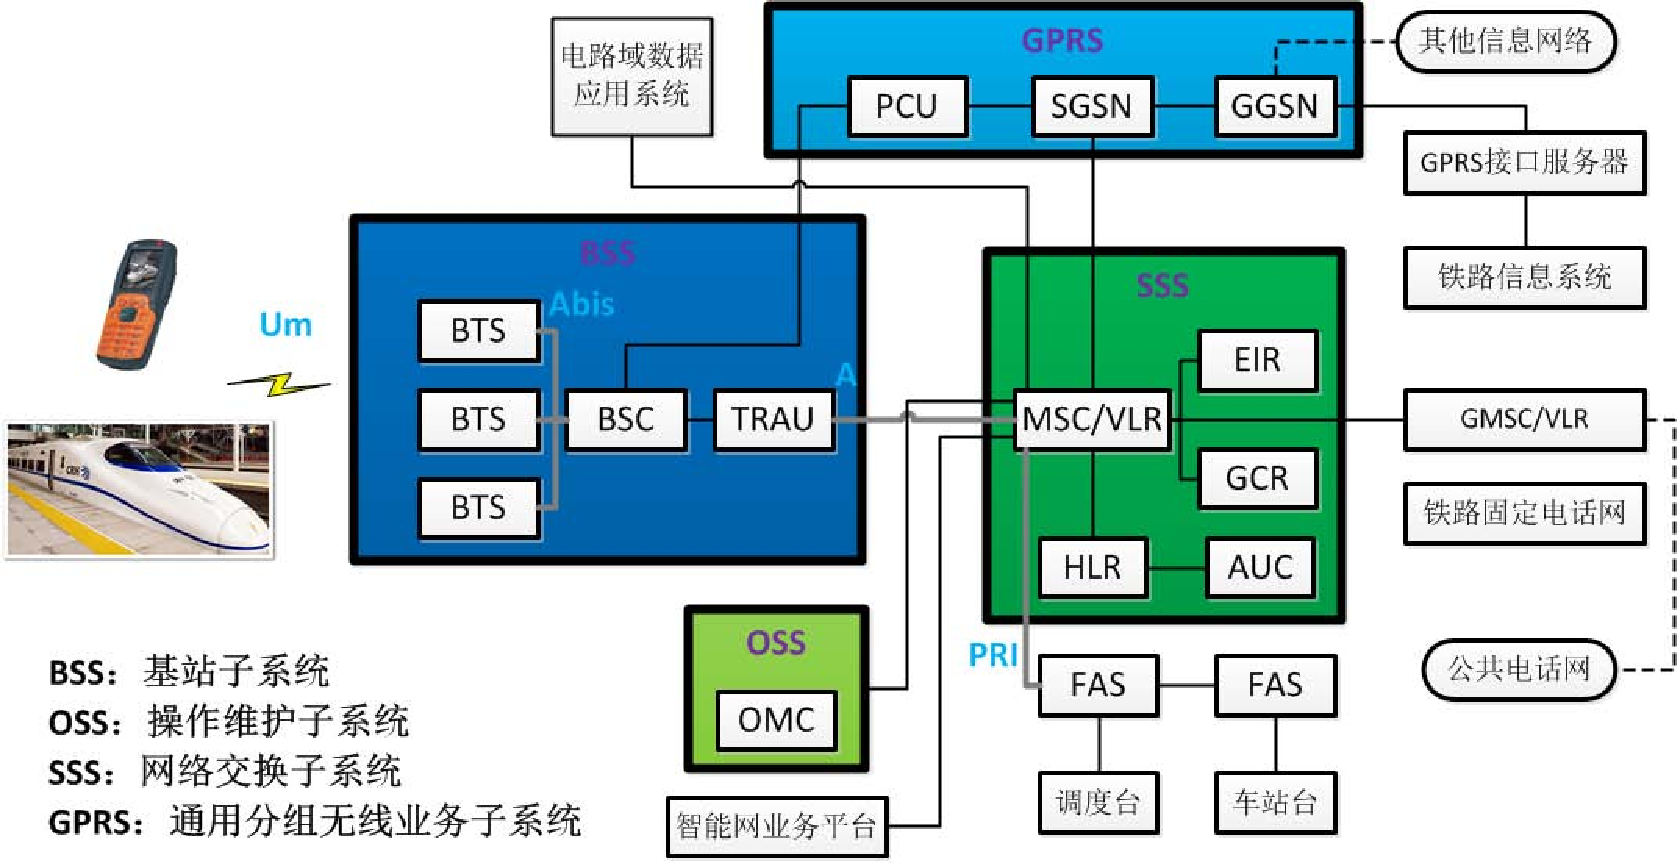
\includegraphics[width=0.9\textwidth]{chap1/gsmr.pdf}
\bicaption[fig:gsmr]{GSM-R网络基本结构}{GSM-R网络基本结构}{Fig}{Architecture of GSM-R networks}
\end{figure}

\subsection{无线局域网络}
\label{sec:80211n}

近年来,无线业务的流量和带宽需求不断提高,使得基于802.11n的无线局域网络(Wireless Local Area Networks, WLANs)经历了快速的发展,同时由于智能手机等移动终端的迅猛发展,802.11n网络将会得到进一步的发展 \cite{Bala2010wifi}。802.11n网络一方面能够有效提升网络性能,同时也使得链路质量的测试与建模更为复杂。

802.11n网络的显著特点是采用了MIMO-OFDM及其相关技术,从而有效地提升网络的传输性能。在物理层方面,多天线技术有效提升网络吞吐量及覆盖范围,同时提高系统的稳定性,以及信道绑定技术等,更好地解决载波侦听、隐藏/暴露终端等问题;在链路层方面,802.11n网络采用帧聚合技术即多个帧共用一个MAC头部,同时降低ACK发送频率及发送/接收开销,提高传输效率,同时采用400ns的短保护间隔,以降低时间开销,并提高链路层吞吐量。

\begin{table}[!htp]
\renewcommand{\arraystretch}{1}
\bicaption[tab:feature]{802.11网络基本参数}{802.11网络基本参数}{Table}{Features and settings of 802.11 networks}
\centering
\begin{threeparttable}[b]
\begin{tabular}{ccccc}
\hline
         & 802.11a  & 802.11b    & 802.11g       & 802.11n \\
\hline
调制方式 & OFDM     & DSSS/CCK   & OFDM DSSS/CCK & SDM/OFDM \\
%\cline{2}
频率     & 5GHz     & 2.4GHz     & 2.4GHz        & 2.4/5GHz \\
%\cline{2}
信道带宽 & 20MHz    & 25MHz      & 25MHz         & 20/40MHz \\
%\cline{2}
传输速率 & 6-54Mbps & 5.5/11Mbps & 1-54Mbps     & 6-600Mbps \\
\hline
\end{tabular}
\end{threeparttable}
\end{table}

首先802.11n网络显著提升了无线局域网络的传输性能、覆盖范围及其兼容性。在传输速率方面,802.11n可以将无线局域网的传输速率由目前802.11a及802.11g提供的54Mbps,提高到300Mbps甚至高达600Mbps。得益于将多天线(Multiple Input Multiple Output, MIMO)与正交频分复用(Orthogonal Frequency Division Multiplexing, OFDM)技术相结合而应用的MIMO-OFDM技术,提高了无线传输质量,也使传输速率得到极大提升,如表 \ref{tab:feature} 所示;在覆盖范围方面,802.11n采用智能天线技术,通过多组独立天线组成的天线阵列,可以动态调整波束,保证让用户接收到稳定的信号,并可以减少其它信号的干扰。因此其覆盖范围可以扩大到好几平方公里,同时使无线局域网的移动性得到极大提高;在兼容性方面,802.11n采用了一种软件无线电技术,它是一个完全可编程的硬件平台,使得不同系统的基站和终端都可以通过这一平台的不同软件实现互通和兼容,这使得WLAN的兼容性得到极大改善。这意味着WLAN将不但能实现802.11n向前后兼容,而且可以实现WLAN与无线广域网络的结合,比如3G 网络。

\begin{table}[!htp]
\renewcommand{\arraystretch}{1}
\bicaption[tab:mcs]{802.11n网络MCS索引}{802.11n网络MCS索引}{Table}{MCS index of 802.11n}
\centering
\begin{threeparttable}[b]
\begin{tabular}{cccccc}
\hline
  \multirow{2}{*}{MCS} & \multirow{2}{*}{Modulation} & \multirow{2}{*}{Code Rate} & \multirow{2}{*}{Rate (Mbps)} & \multicolumn{2}{c}{Sensitivity (dBm)} \\
\cline{5-6}
  & & & & Typical & Max \\
\hline
  0 & BPSK & 1/2 & 6.5 & -94 & -85 \\
%\cline{2}
  1 & QPSK & 1/2 & 13.0 & -92 & -82 \\
%\cline{2}
  2 & QPSK & 3/4 & 19.5 & -90 & -80 \\
%\cline{2}
  3 & 16 QAM & 1/2 & 26.0 & -87 & -77 \\
%\cline{2}
  4 & 16 QAM & 3/4 & 39.0 & -84 & -73 \\
%\cline{2}
  5 & 64 QAM & 2/3 & 52.0 & -79 & -69 \\
%\cline{2}
  6 & 64 QAM & 3/4 & 58.5 & -78 & -68 \\
%\cline{2}
  7 & 64 QAM & 5/6 & 65.0 & -76 & -67 \\
\hline
\end{tabular}
\end{threeparttable}
\end{table}

另一方面,802.11n网络链路质量的测试与建模更为复杂,如表 \ref{tab:mcs} 所示。第一,802.11n网络的多种配置提高了链路质量测试的复杂度,需要对所有可能的物理层与链路层配置进行采样测试,同时使得链路质量的建模变得复杂;第二,802.11n网络的链路质量与信道状态(Packet Delivery Ratio - Received Signal Strength, PDR-RSS)模型呈现过渡窗口,而并非传统无线网络中的近似线性关系;第三,移动网络的信道状态与链路质量更容易受到无线传播环境及通信终端的移动性的影响,从而影响到链路质量测试与建模的精度。
%
%\begin{figure}[!htp]
%\centering
%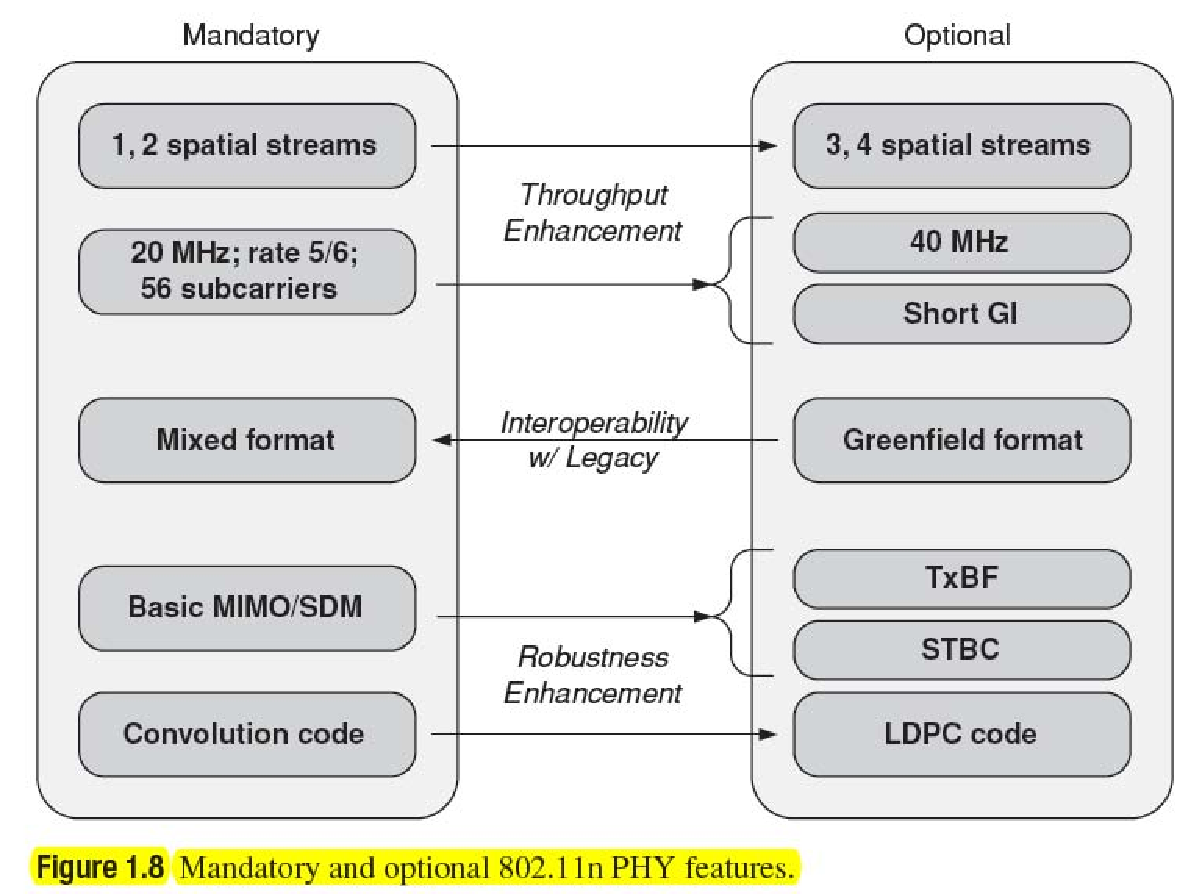
\includegraphics[width=0.5\textwidth]{chap1/PHYfeather.pdf}
%\bicaption[fig:phyfeather]{802.11n网络PHY特性}{802.11n网络PHY特性}{Fig}{Feather of 802.11n Networks}
%\end{figure}
%
%\subsubsection{物理层}
%\begin{itemize}
%  \item Spatial Diversity
%  \item Channel Bonding
%\end{itemize}
%
%
%\begin{figure}[!htp]
%\centering
%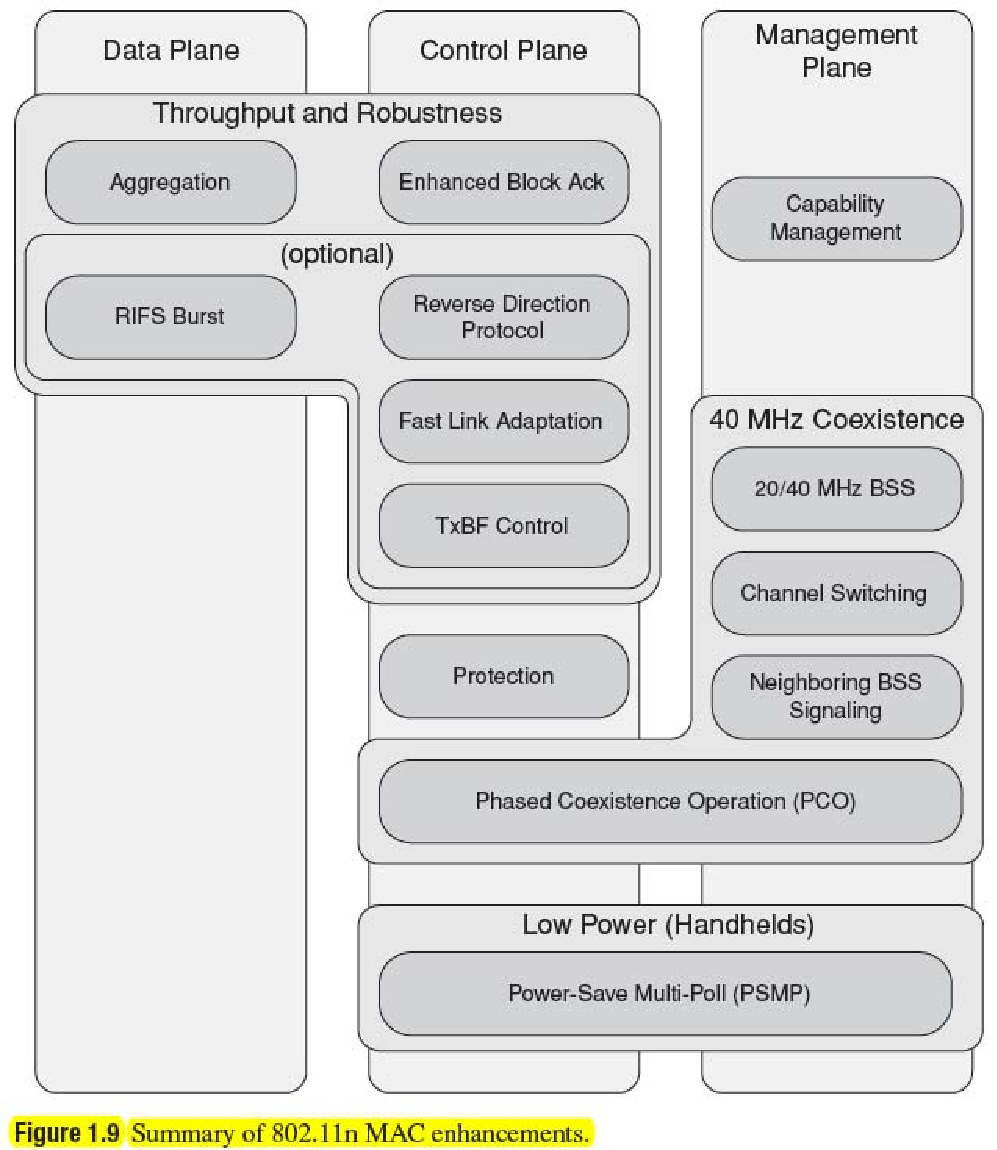
\includegraphics[width=0.5\textwidth]{chap1/MACfeather.pdf}
%\bicaption[fig:macfeather]{802.11n网络MAC特性}{802.11n网络MAC特性}{Fig}{Feather of 802.11n Networks}
%\end{figure}
%
%\subsubsection{链路层}
%\begin{itemize}
%  \item Frame Aggregation
%  \item Streamlined ACK
%\end{itemize}

%\begin{table}[!htp]
%\renewcommand{\arraystretch}{1}
%\bicaption[tab:mcs]{802.11n网络MCS索引}{802.11n网络MCS索引}{Table}{MCS index of 802.11n}
%\centering
%\begin{threeparttable}[b]
%\begin{tabular}{c|c|c|ccc}
%\hline
%  Channel & MCS & Rate(Mbps) & $\beta_-$ & $\beta_0$ & $\beta_+$ \\
%\hline
%  \multirow{8}{*}{HT20/LGI} & 0 &  6.5 & -70 & -65 & -60 \\
%\cline{2}
%                            & 1 & 13.0 & -70 & -65 & -60 \\
%\cline{2}
%                            & 2 & 13.0 & -70 & -65 & -60 \\
%\cline{2}
%                            & 3 & 13.0 & -70 & -65 & -60 \\
%\cline{2}
%                            & 4 & 13.0 & -70 & -65 & -60 \\
%\cline{2}
%                            & 5 & 13.0 & -70 & -65 & -60 \\
%\cline{2}
%                            & 6 & 13.0 & -70 & -65 & -60 \\
%\cline{2}
%                            & 7 & 13.0 & -70 & -65 & -60 \\
%\hline
%  \multirow{8}{*}{HT20/SGI} & 0 &  6.5 & -70 & -65 & -60 \\
%\cline{2}
%                            & 1 & 13.0 & -70 & -65 & -60 \\
%\cline{2}
%                            & 2 & 13.0 & -70 & -65 & -60 \\
%\cline{2}
%                            & 3 & 13.0 & -70 & -65 & -60 \\
%\cline{2}
%                            & 4 & 13.0 & -70 & -65 & -60 \\
%\cline{2}
%                            & 5 & 13.0 & -70 & -65 & -60 \\
%\cline{2}
%                            & 6 & 13.0 & -70 & -65 & -60 \\
%\cline{2}
%                            & 7 & 13.0 & -70 & -65 & -60 \\
%\hline
%\end{tabular}
%\end{threeparttable}
%\end{table}


\section{通信质量测试}
\label{sec:measure}

对于高速移动网络GSM-R与无线局域网络802.11n通信质量测试而言,其目标都是实现系统可靠性与网络传输性能的有效平衡,但是两者的侧重点不同,前者主要保证网络的可靠运行,而后者主要实现传输性能的提升。无线网络通信质量通常由信道状态与链路质量进行衡量,而信道状态是链路质量的基础,因此对于GSM-R网络而言,其关键是如何在高速移动情况下实现信道状态的可靠估计,同时在保证测试精度的前提下尽量降低测试开销,进而完成上层的链路质量测试以保证系统可靠性;而对于移动802.11n网络,由于其移动性与多配置的特性,主要难点是如何实现实时的链路质量测试与建模,从而实现不同网络状态下网络的有效配置,以提高网络传输性能。

\subsection{物理层信道状态估计}
\label{sec:phy}

无线传播测量与信道状态估计在移动网络中发挥重要作用,并广泛应用于其他上层应用中,例如无线覆盖评估、信道接入、功率控制及小区切换等 \cite{Austin1994}\cite{itoh2002performance}\cite{zhang1996analysis}\cite{zhu2005performance}。文献 \cite{andersen1995propagation} \cite{sarkar2003survey} 给出了无线网络中无线传播模型及其测试方法,文献 \cite{Ostlin2008itu} 以国际电信联盟(International Telecommunication Union, ITU)相关规定为基础提出点到面无线传输服务的无线预测模型,\cite{Akhoondzadeh2007modifi} 和 \cite{medeisis2000use} 分别基于最小均方差和Levenberg-Marquardet方法提出改进Okumura-Hata传播模型。以上的无线传播模型与测试方法主要集中于路径损耗与阴影衰落,当考虑到移动无线网络中的多径衰落时,主要问题是如何对接收信号强度进行估计,以准确反映网络当前的链路质量。

针对这一问题,William C. Y. Lee在1985年提出移动网络信号强度采样算法 \cite{lee1985estimate},该算法分析了瑞利衰落情况下接受信号强度本地均值的估计问题,并给出合适的统计区间与采样点数的参数设置。Mark D. Austin在其蜂窝网络的切换算法中对莱斯衰落条件下的采样算法进行了推导 \cite{Austin1994},得到统计区间与采样点数的近似解,但是该算法过程复杂且计算量较大。David de la Vega在2009年提出通用Lee氏采样算法 \cite{Vega2009},在不需要知道多径衰落具体分布的条件下,利用实测采样信号进行估计,得到实际网络环境所需要的统计区间与采样点数。由于高速铁路无线环境的复杂性及其对安全性的特殊要求,以上的本地均值估计算法难以在较低的测试开销条件下实现可靠的测试精度,不符合高铁环境实时测试的要求,因此无法直接应用于GSM-R网络中。

由于高速铁路沿线地形复杂多变,一条线路通常会经过山地、平原、隧道和高架等地形,从而造成GSM-R网络无线传播环境的复杂性。同时高速铁路无线传播环境大多较为平坦,同时为了尽量保证GSM-R网络的可靠性,基站位置通常距离高铁线路很近,而且小区半径一般设置为3-6km,从而造成移动终端与基站之间一般存在直射路径(Line of Sight, LOS),因此GSM-R网络的无线传播应该刻画为莱斯衰落。对于莱斯衰落信道的参数估计已有大量相关工作,包括基于学习训练机制 \cite{bjornson2010framework}、最大似然估计(Maximum Likelihood, ML) \cite{sijbers1998maximum} 以及期望最大化算法(Expectation Maximization, EM)\cite{marzetta1995algorithm}。因此GSM-R网络的信道状态估计问题实为莱斯衰落信道下本地均值估计,如何通过莱斯衰落参数估计,确定信道状态测试的采样参数。

\subsection{链路层链路质量测试}
\label{sec:mac}

无线网络中基于实测数据的PDR-RSS模型存在大量研究,多数早期的工作主要针对静态无线网络中的离线PDR-RSS模型 \cite{kolar2011mesh} \cite{reis2006model},同时实测PDR-RSS模型广泛应用于其他上层应用中,包括容量分析 \cite{kashyap2007capacity} 和速率控制 \cite{chen2011ram} \cite{judd2008efficient} 等。文献 \cite{10.1109/TMC.2009.87} 通过实验与仿真的结合,提出移动无线网络的可重复测量方法,文献 \cite{kim2010sybot} 同样提出针对移动网络的频谱测量方法,但是只对RSS进行测量而忽略链路质量。以上的移动无线网络测量方法都基于传统802.11a/b/g网络,而无法直接应用于802.11n网络中。由于802.11n网络采用MIMO-OFDM技术,导致PDR-RSS模型存在过渡窗口,从而增加了链路质量测试与建模的复杂度。近期许多工作针对802.11n 网络的实验特性进行了详细分析 \cite{Halperin2010predictable} \cite{k.rayanchu:fluid:},其中文献 \cite{Halperin2010predictable} 利用802.11n 网络的MIMO-OFDM 特性提出基于信道状态信息(Channel State Information, CSI)的链路质量预测模型;文献 \cite{k.rayanchu:fluid:} 针对信道绑定技术,分析了信道带宽对无线局域网络性能的影响。以上针对802.11n网络的工作并未针对移动性进行分析,同时主要针对物理层而忽略链路层的影响。

信道状态与链路质量及其模型广泛应用于速率控制算法中 \cite{kim2009experimental} \cite{Pefkianakis:2010} \cite{zhang2008practical} \cite{Li:2012:ERA:2348543.2348585},许多算法应用于Linux平台无线驱动中,例如采用Minstrel算法 \cite{minstrel} 的\textit{mac80211} 及Atheros \cite{wong2008wireless}的\textit{ath9k} 无线驱动,但是以上的算法都采用固定指数加权平均(Exponential Weighted Moving Average, EWMA)进行链路质量测试,仅适用于静态802.11网络。针对移动无线网络的速率控制算法主要针对RSS测量 \cite{chen2011ram} \cite{judd2008efficient},并利用静态PDR-RSS模型进行链路质量预测,但是其预测精度容易受802.11n网络的MIMO-OFDM配置的影响。许多上层应用考虑到在线PDR测试算法,比如入侵信号检测 \cite{5620919} 与拥塞控制 \cite{floyd2000equation} 等,但是并不考虑链路质量建模与速率控制问题。以上速率控制算法主要利用静态PDR-RSS模型 \cite{kashyap2007capacity} \cite{kolar2011mesh} \cite{reis2006model},同时只利用单一指标,即链路层PDR或物理层RSS,进行链路质量预测与速率控制 \cite{judd2008efficient} \cite{zhang2008practical}。

\section{本章小结}

本章主要介绍了移动网络通信质量测试,针对移动网络中可靠性与传输性能的有效平衡,提出信道状态与链路质量测试问题。首先对于高速移动网络GSM-R而言,首要问题是保证系统的可靠性,因此需要对无线接口进行实时监测,但由于移动终端的高速移动性及传播环境的复杂性,对信道状态估计的精度与开销带来极大挑战。其次在无线局域网络中,MIMO-OFDM技术能够有效地提升网络的传输性能,但同时其多配置的特性给链路质量测试与建模带来新的问题,而通信终端的移动性又进一步降低了链路质量测试的精度。因此本文针对移动网络中信道状态及链路质量测试问题,提出动态测试算法以根据当前网络状态调整测试参数,从而保证网络的可靠运行及传输性能。本文的章节安排如下,第二章主要介绍信道状态采样与估计,针对GSM-R网络的高速移动性与传播环境复杂性,提出接收信号强度动态测试算法,在保证一定测试精度的条件下降低测试开销,并通过系统设计与实现对该算法进行评估。第三章介绍链路质量测试与建模,主要解决移动802.11n网络中MIMO-OFDM配置及移动性对链路质量测试与建模带来的问题,提出在线测试与建模框架,在保证系统可靠性的前提下尽量提高系统吞吐量,最后通过系统实现与实验测试对其测试及传输性能进行评估。

%%==================================================
%% chapter02.tex for SJTU Master Thesis
%% based on CASthesis
%% modified by wei.jianwen@gmail.com
%% version: 0.3a
%% Encoding: UTF-8
%% last update: Dec 5th, 2010
%%==================================================

% \bibliographystyle{sjtu2} %[此处用于每章都生产参考文献]

\chapter{信道状态采样与估计}
\label{chap:phy}

安全始终是高速铁路发展过程中的首要目标,而GSM-R网络则是保证高铁系统安全性的重要环节,因此有必要对GSM-R网络进行在线实时测试,在确保GSM-R网络正常通信的基础之上,保证整个高铁系统的稳定运行。但是由于高铁系统具有较为特殊的无线传播环境,传统的信号强度测试算法无法直接应用于GSM-R网络测试中,例如高铁线路周围地形复杂多变以及列车处于高速运行状态,这就要求GSM-R网络信号强度测试算法必须具有实时高效的特点,以适应高速铁路的特殊要求。

\section{问题描述}
\label{sec:problem2}

\begin{figure}[!htp]
\centering
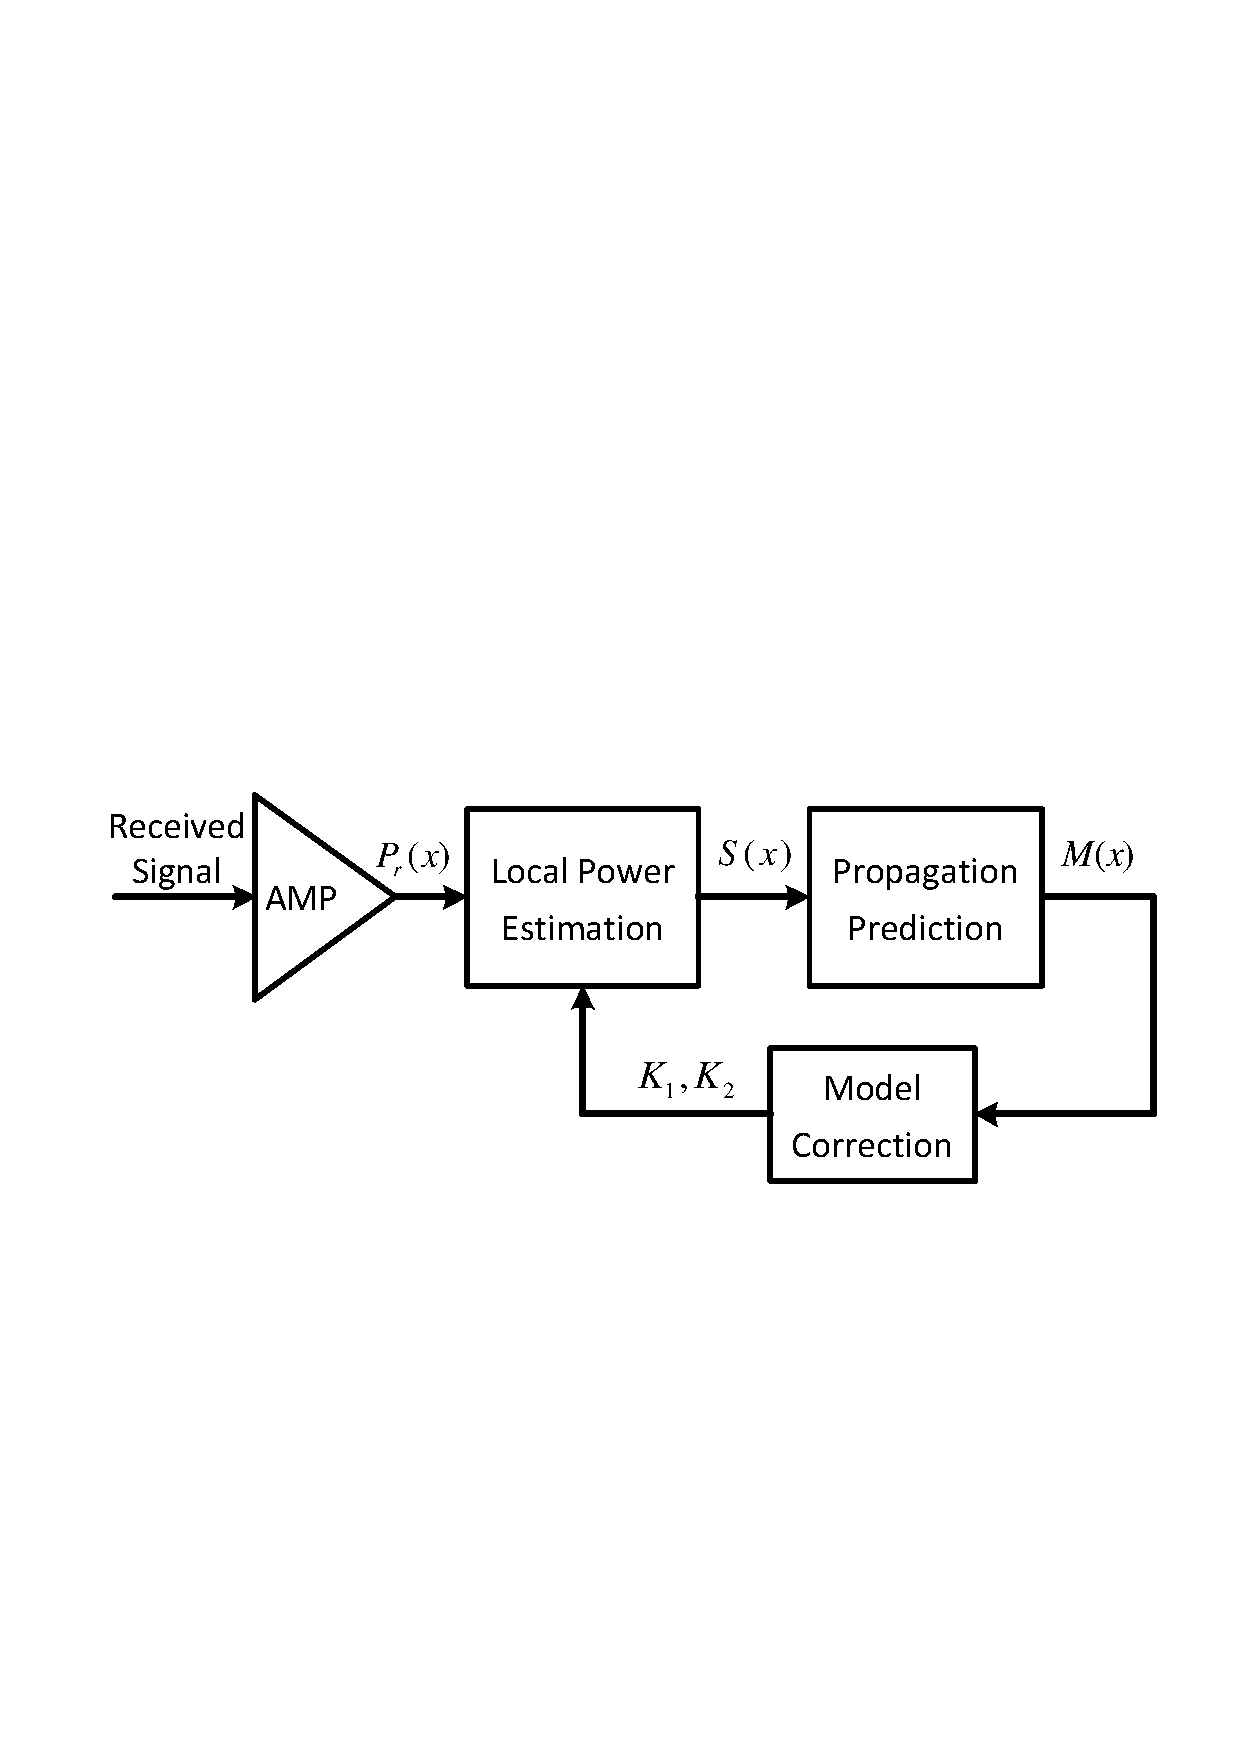
\includegraphics[width=4in]{chap2/measurement.pdf}
\bicaption[fig:measurement]{接收信号强度测试过程}{接收信号强度测试过程}{Fig}{Basic Procedures of Radio Propagation Measurement}
\end{figure}

无线网络接收信号强度测试过程如图 \ref{fig:measurement} 所示,测试系统通过包络检测得到接收信号强度,然后通过信号动态采样算法,得到当前阴影衰落与多径衰落信息,一方面用来对网络通信状态进行评估,另一方面作为网络越区切换的判断依据。同时根据采样数据进行无线传播预测,对网络的覆盖情况进行评估,最后对估计算法与预测模型进行参数修正。

\subsection{现有工作}
\label{sec:current3}

\begin{figure}[!htp]
\centering
    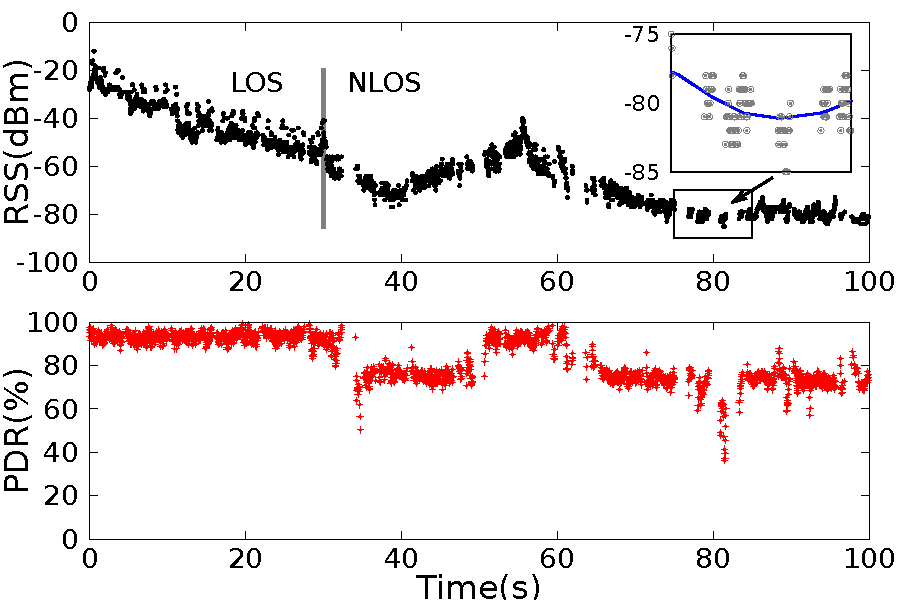
\includegraphics[width=5in]{chap2/time.pdf}
\bicaption[fig:timevary]{移动无线网络时变特性}{移动无线网络时变特性}{Fig}{Time varying of RSS in mobile wireless networks}
\end{figure}

移动无线网络信号强度测试的一个基本问题是本地均值的可靠估计,即如何确定合适的采样参数以准确地获取当前信号强度,同时在测试精度与开销之间实现合理平衡。移动无线网络接收信号强度通过特定统计区间内一定数量的采样点数的算术平均获得,因此采样频率决定了信号强度的测试精度与开销,因此需要根据无线传播环境的变化对信号的采样频率进行实时调整,对于GSM-R网络而言合理有效的采样精度与开销的平衡尤为重要。

如图 \ref{fig:timevary} 所示,移动无线网络接收信号强度具有明显的时变特性,其中包括大尺度衰落和小尺度衰落,如果信号采样的统计区间过长或采样频率过低,系统将无法对小尺度衰落作出合理评估,从而难以保证可靠的数据传输;相反,如果统计区间过段或采样频率过高,大尺度衰落和小尺度衰落难以有效区分,从而导致网络状态的不稳定,例如接收信号强度在切换门限附近波动造成的乒乓切换效应。

William C. Y. Lee在1985年最先提出移动网络信号强度采样算法,即Lee氏采样算法 \cite{lee1985estimate},该算法以移动网络无线传播传播模型为基础,在无线传播环境服从瑞利衰落的假设条件下,推导出信号强度的本地均值测量中的统计区间长度与采样点数。Mark D. Austin在其蜂窝网络的切换算法中对莱斯衰落条件下的采样算法进行了推导 \cite{Austin1994},得到统计区间与采样点数的近似解,但是该算法过程复杂且计算量较大。David de la Vega在2009年提出通用Lee氏采样算法 \cite{Vega2009},在不需要知道多径衰落具体分布的条件下,利用实测采样信号进行估计,得到实际网络环境所需要的统计区间与采样点数。由于高速铁路无线环境的复杂性及其对安全性的特殊要求,以上的本地均值估计算法难以在较低的测试开销条件下实现可靠的测试精度,不符合高铁环境实时测试的要求,因此无法直接应用于GSM-R网络中。

\subsection{存在问题}
\label{sec:prob3}

\begin{itemize}
  \item \textbf{高速移动特性}
  GSM-R网络处于高速运行状态,相同情况下需要对接收信号强度进行更为频繁的采样,同时不能够影响到网络的正常通信。
  \item \textbf{无线传播环境}
  GSM-R网络一般存在直射路径,因此应当采用莱斯信道对GSM-R网络的无线传播环境进行刻画,由于莱斯信道衰落参数及其估计算法的复杂性,
  The basic consideration in local power estimation is the sampling frequency which is determined by the length of statistical intervals and number of averaging samples. The received signal strength of wireless propagation is influenced by the environments, so the local mean power estimation should be dynamic to the networks status, especially for GSM-R networks. Fig.~\ref{fig:time} demonstrates the time varying and location difference characteristics of received signal strength $P_r(x)$ in mobile networks, which indicates the facts that Fig.~\ref{fig:timevary}: certain received signal strength carve contains both long-term and short-term fluctuation; Fig.~\ref{fig:cdfrss}: the overall received signal strength shows different characteristics for different routes. Since the received signal strength $P_r(x)$ is changing in both large and small time scale, the local mean power estimation should also be adaptive to this fluctuation.
\end{itemize}

\begin{figure}[!htp]
\centering
    \label{}
    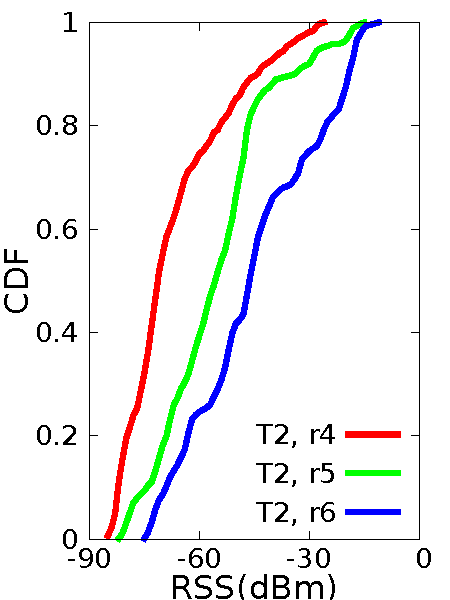
\includegraphics[width=2in]{chap2/cdfrss.pdf}
\bicaption[fig:cdfrss]{移动无线网络位置差异性}{移动无线网络位置差异性}{Fig}{Location differences of RSS in mobile wireless networks}
\end{figure}


\section{无线传播模型}
\label{sec:channelmodel}

由于高速铁路沿线地形复杂多变,一条线路通常会经过山地、平原、隧道和高架等地形,如图 \ref{fig:terrain} 所示,从而造成GSM-R网络无线传播环境的复杂性。同时图 \ref{fig:terrain} 中可以看出,高速铁路无线传播环境大多较为平坦,同时为了尽量保证GSM-R网络的可靠性,基站位置通常距离高铁线路很近,而且小区半径一般设置为3-6km,从而造成移动终端与基站之间一般存在直射LOS路径,因此GSM-R网络的无线传播应该刻画为莱斯衰落。

\begin{figure}[!htp]
\centering
\subfigure[高架]{
    \label{fig:viaduct}
    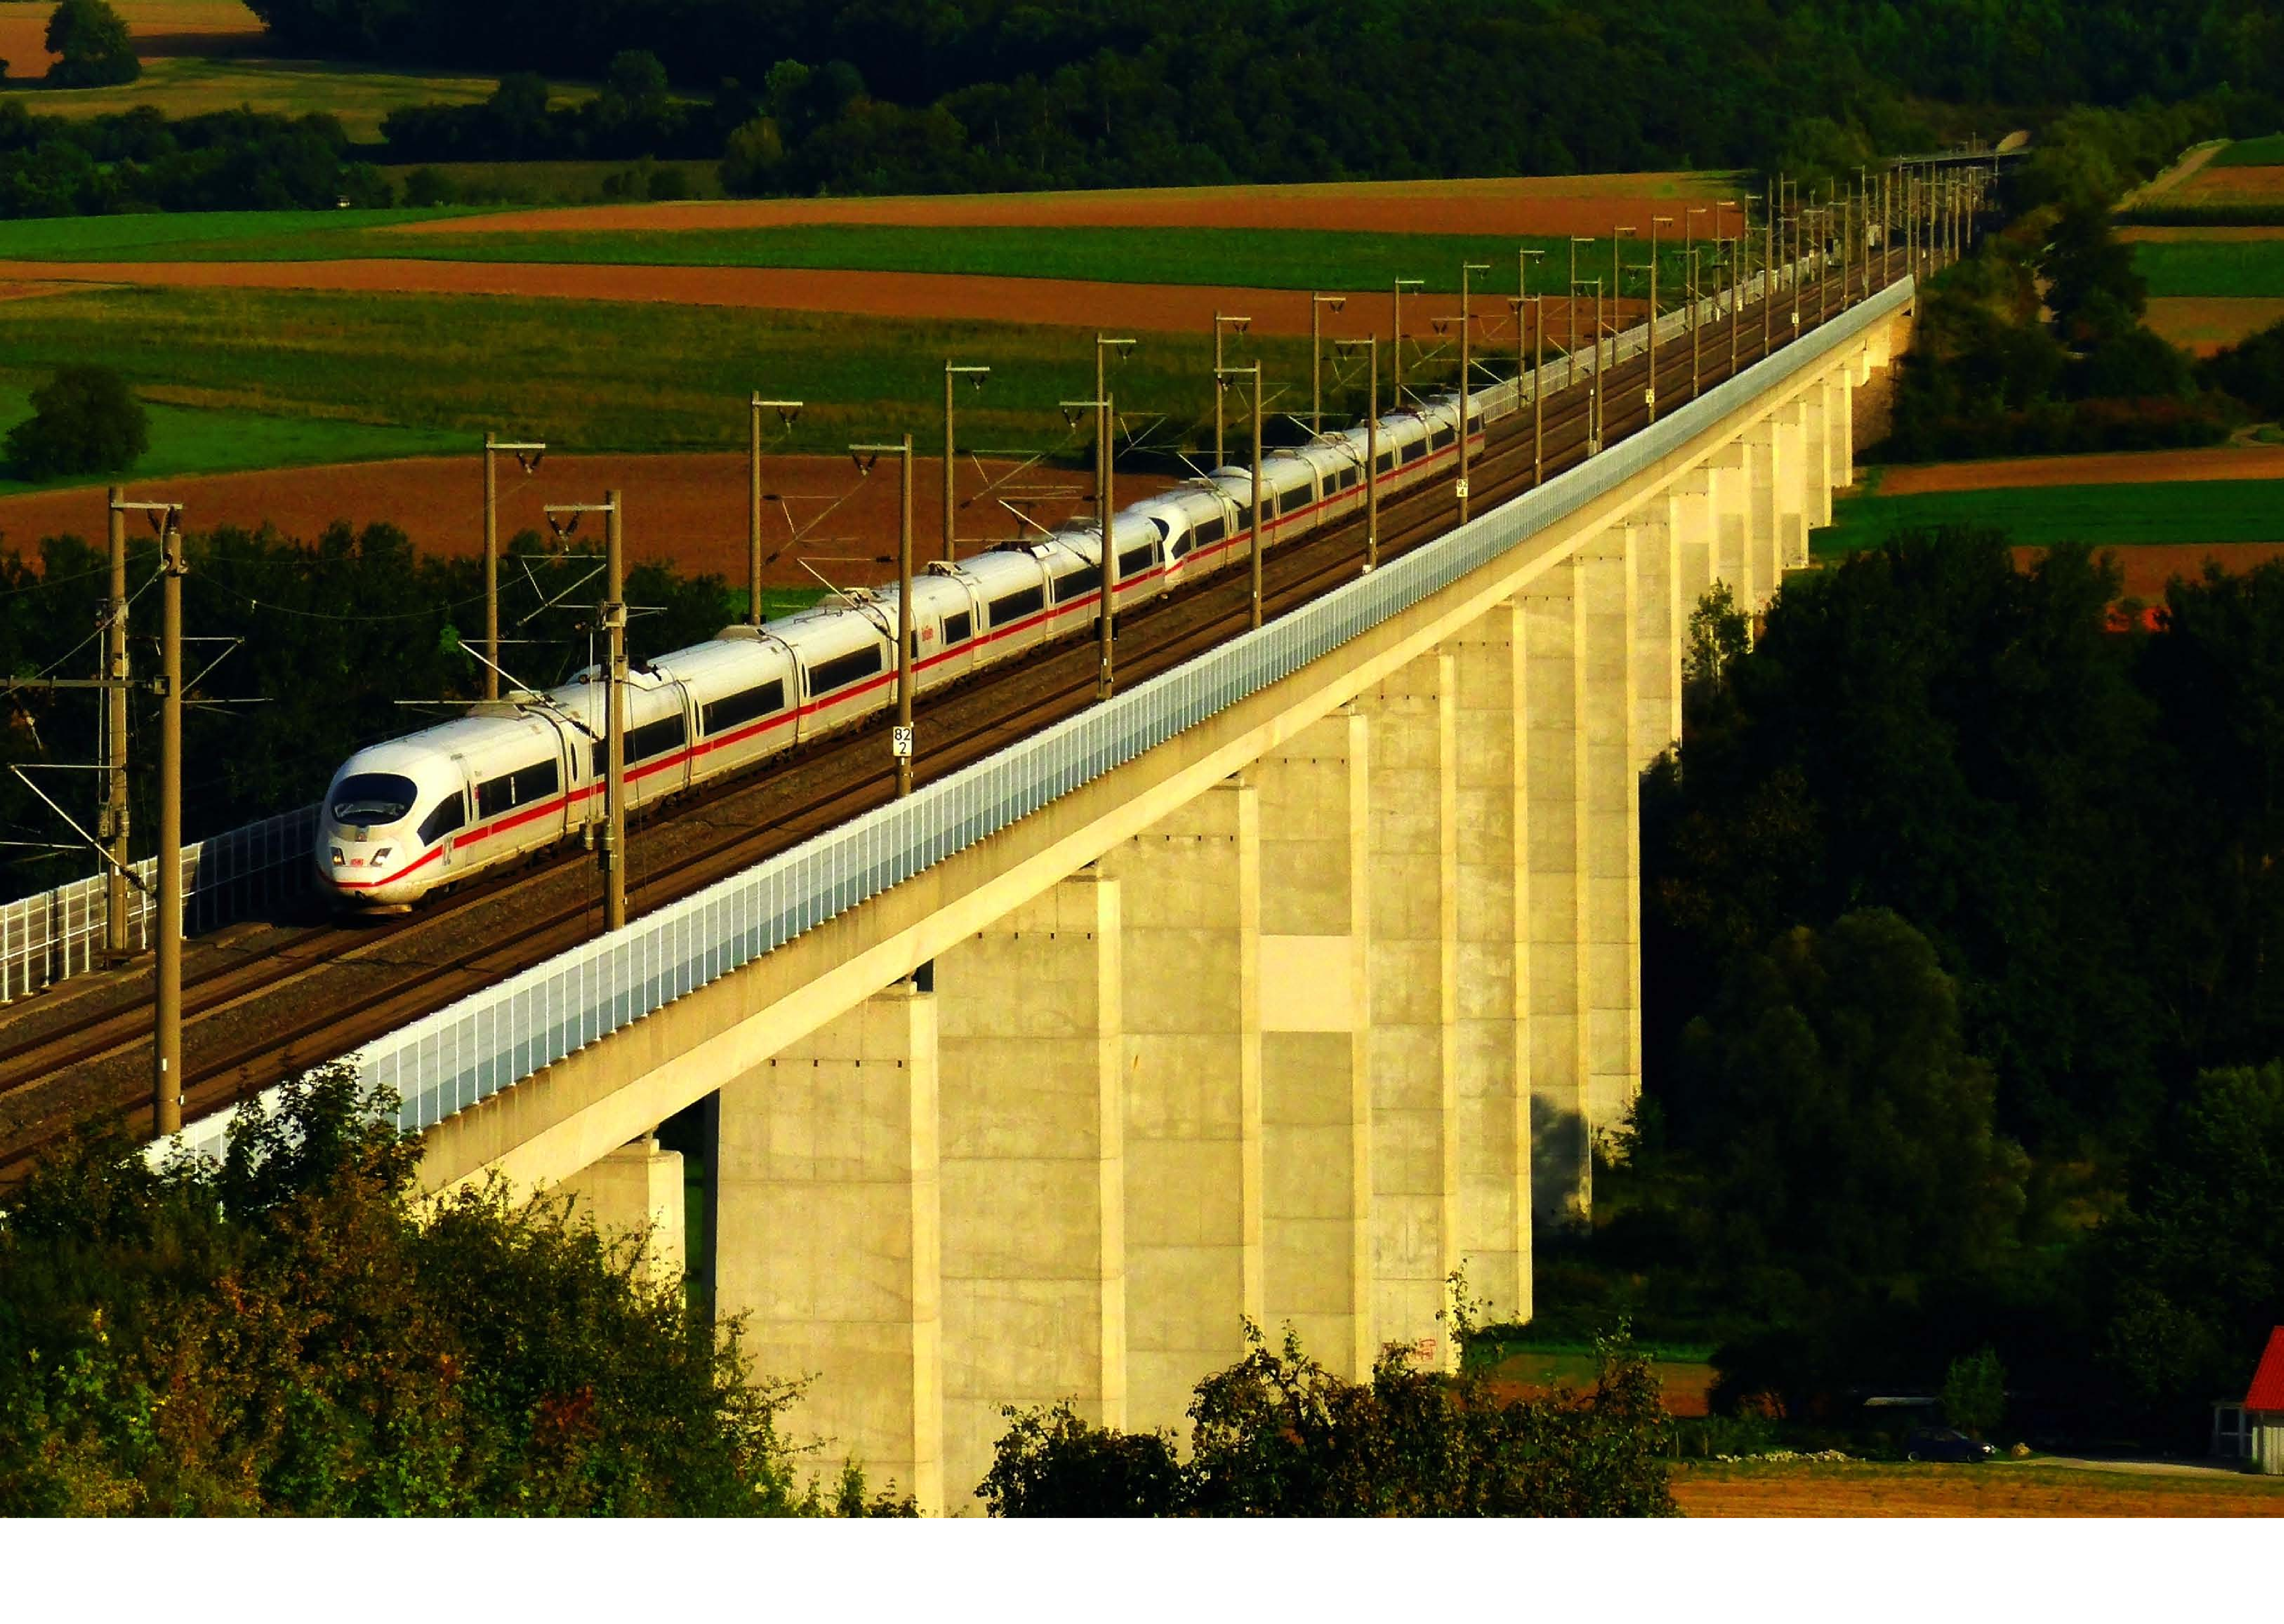
\includegraphics[width=2.5in]{chap2/viaduct.pdf}}
    \hspace{1cm}
\subfigure[隧道]{
    \label{fig:tunnel}
    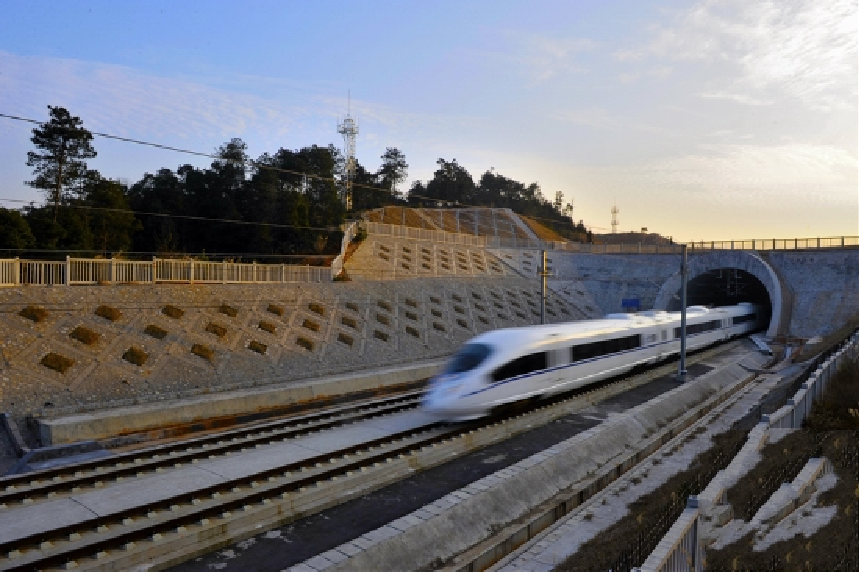
\includegraphics[width=2.5in]{chap2/tunnel.pdf}}
\hspace{1in}
\centering
\subfigure[山区]{
    \label{fig:mountain}
    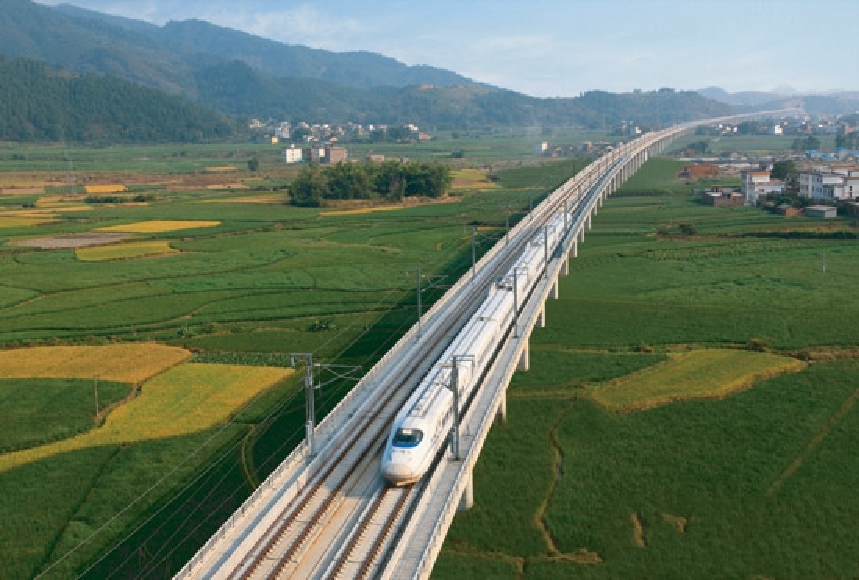
\includegraphics[width=2.5in]{chap2/mountain.pdf}}
    \hspace{1cm}
\subfigure[平原]{
    \label{fig:plain}
    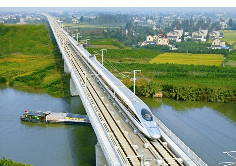
\includegraphics[width=2.5in]{chap2/plain.pdf}}
%\hspace{1in}
%\centering
%\subfigure[车站]{
%    \label{fig:hongqiao}
%    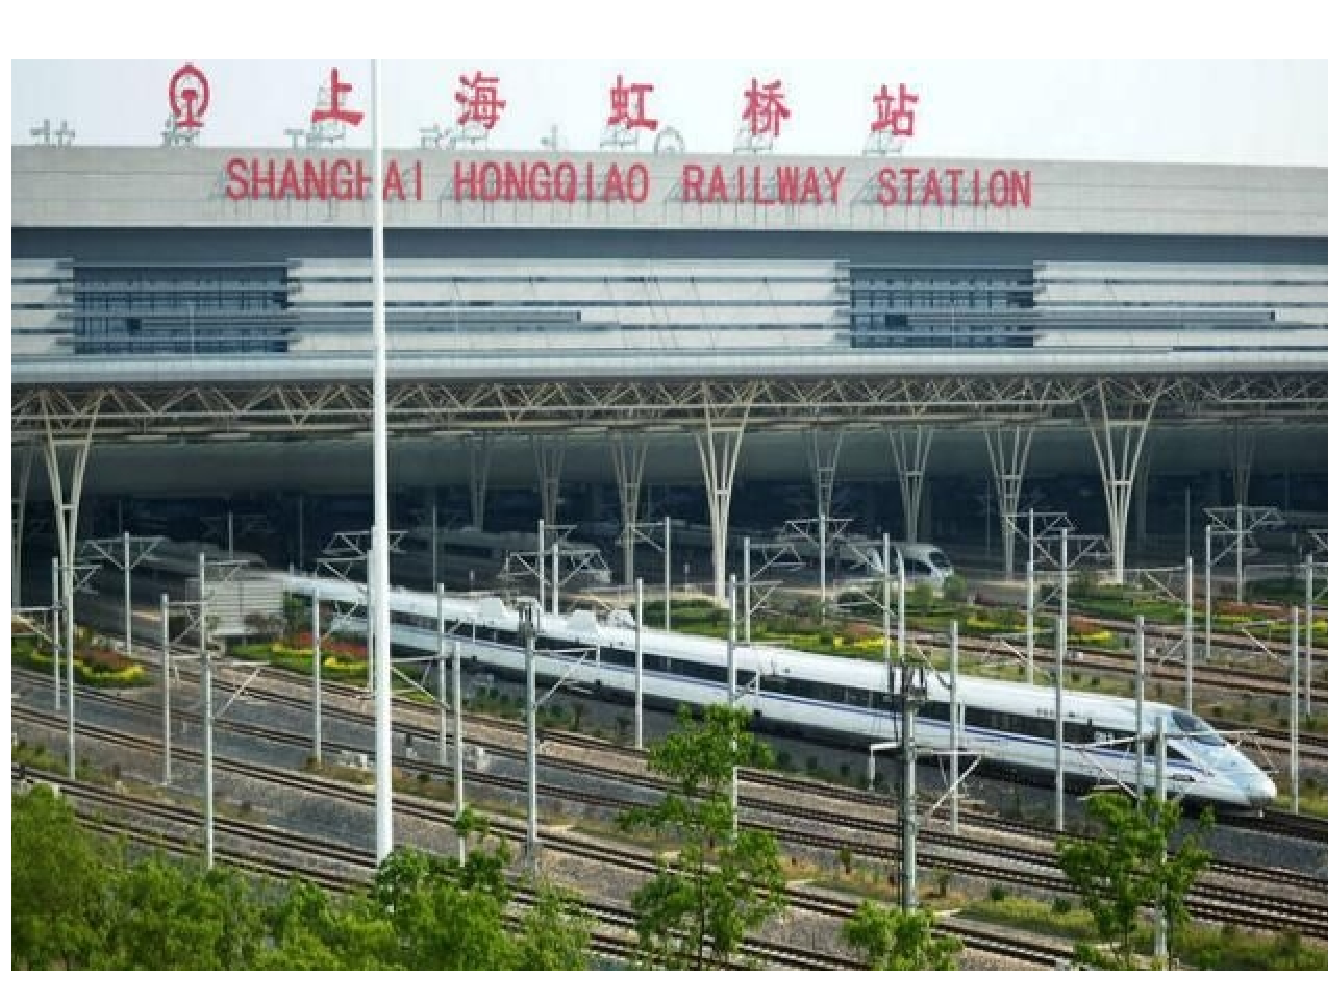
\includegraphics[width=2.5in]{chap2/hongqiao.pdf}}
%    \hspace{1cm}
%\subfigure[基站]{
%    \label{fig:qingzang}
%    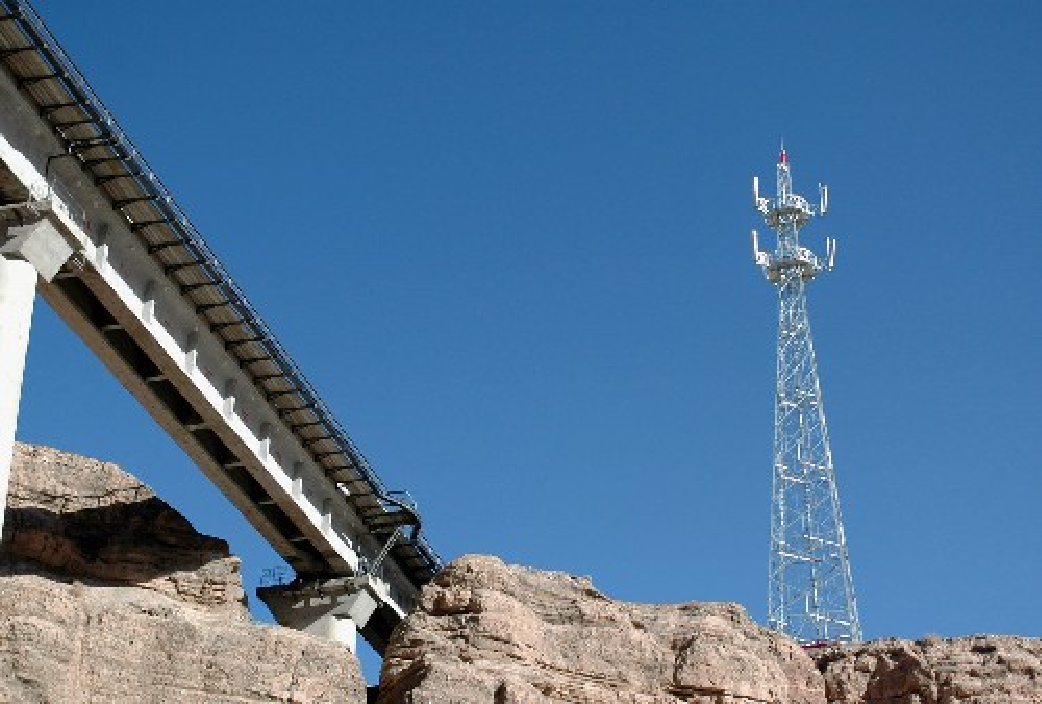
\includegraphics[width=2.5in]{chap2/qingzang.pdf}}
\bicaption[fig:terrain]{GSM-R网络无线传播环境}{GSM-R网络无线传播环境}{Fig}{Radio Propagation Environments and terrains of GSM-R Networks}
\end{figure}

在GSM-R网络空中接口的无线通信中,接收信号强度可以视为阴影衰落与多径衰落的叠加,如式(\ref{equa:p_r1})所示,
\begin{equation}
    p_{r}^{2}(x) = s(x)h(x)
\label{equa:p_r1}
\end{equation}
其中$s(x)$为阴影衰落,服从高斯过程;$h(x)$为多径衰落,服从复高斯过程;$x$可以视为移动台与基站之间距离,利用列车运行速度公式可以转化为时间变量。如图 \ref{fig:train} 所示,GSM-R网络中移动台与基站间距离$d$在10m左右,因此$\Delta x=\sqrt{d^2+v_{train}^2\cdot \Delta t^2}$ 可以简化为$\Delta x=v_{train}\cdot \Delta t$。同时式(\ref{equa:p_r1})可以表示为对数域形式,如式(\ref{equa:P_r2})所示,
\begin{equation}
P_{r}(x) = S(x) + H(x)
\label{equa:P_r2}
\end{equation}
其中$P_r(x)$、$S(x)$、$H(x)$分别为接收功率与信号衰落在对数域的表示,即$P_r(x):=10\log(p_{r}^{2}(x))$,$S(x):=10\log(s(x))$,$H(x):=10\log(h(x))$。

\begin{figure}[!htp]
\centering
    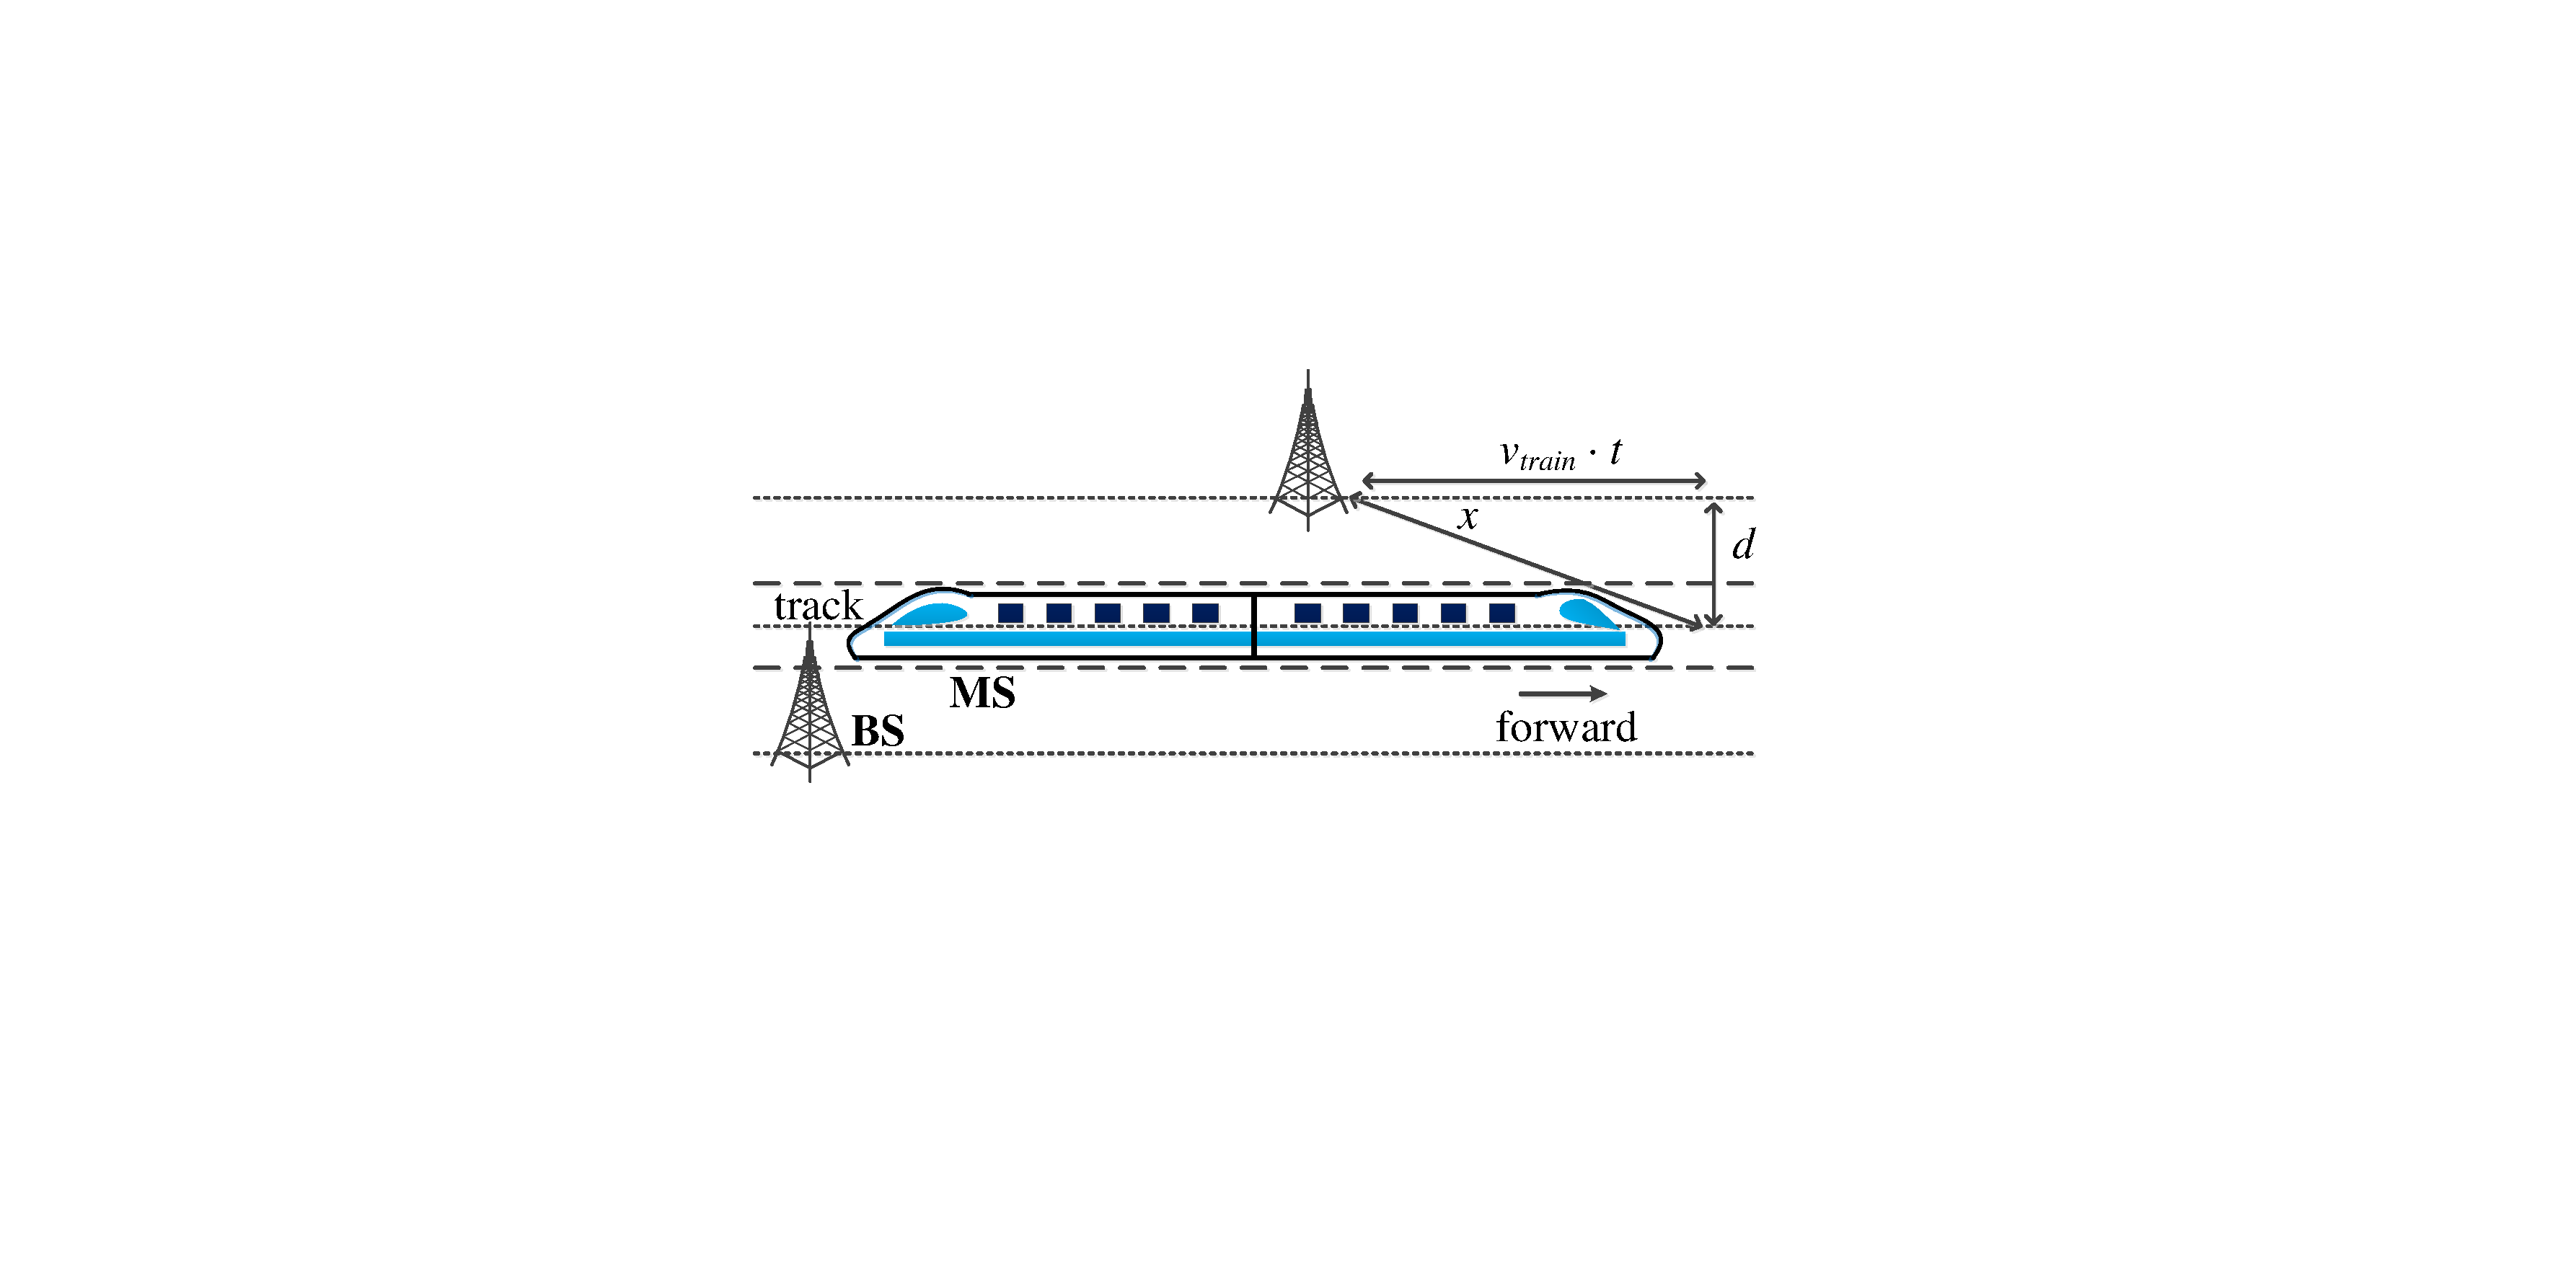
\includegraphics[width=5in]{chap2/train.pdf}
\bicaption[fig:train]{GSM-R网络移动台与基站间距离}{GSM-R网络移动台与基站间距离}{Fig}{The distance between MS and BS in GSM-R networks}
\end{figure}

\subsection{阴影衰落}
\label{sec:shadow}

阴影衰落可用如式(\ref{equa:shadow})所示的高斯过程表示
\begin{equation}
    s(x) \sim N\left( m(x),\sigma_s^2 \right)
\label{equa:shadow}
\end{equation}
其中均值$m(x)$主要受路径损耗影响,方差$\sigma_s^2$受地形因素影响。 文献 \cite{sarkar2003survey} 综合基站发射功率、移动台接收灵敏度以及无线传播环境的影响,给出$m(x)$的基本模型并被广泛应用,表示为式(\ref{equa:pathloss})
\begin{equation}
    M(x)= K_1+K_2\log(x)
\label{equa:pathloss}
\end{equation}
其中$M(x):=20\log(m(x))$为$m(x)$的对数形式,$K_1$主要与基站发射功率、天线增益及线路损耗有关,$K_2$为地形因子并随着无线传播环境的不同而变化 \cite{hata1980empirical}\cite{medeisis2000use}。$S(x)$的空间相关性,即其自相关函数,主要与地形因素有关,表示为式(\ref{equa:multipath}) \cite{gudmundson1991correlation}。
\begin{equation}
    R_{s}(x) = \sigma_{s}^2\exp\left(-\frac{\Delta x}{x_0}\right)
\label{equa:multipath}
\end{equation}
其中$\sigma_s$为$S(x)$的方差,通常在4到12dB间取值;$x_0$为相关距离,根据传播环境的不同一般为10m到500m \cite{tepedelenlio?lu2001estimation};$\Delta x$为相对距离,可以通过移动台运行速度即采样时间间隔获得,即$\Delta x = v_{train}\cdot\Delta t$。在阴影衰落模型中,地形因子$K_2$、阴影衰落方差$\sigma_s$及自相关距离$x_0$都与无线传播环境有关,同时影响到上层应用的参数设置,例如小区切换算法中的切换门限值的选择。

\subsection{多径衰落}
\label{sec:multipath}

多径衰落是由于信号的衍射和散射而导致的接收信号强度的瞬时波动,所以移动终端的接收信号强度是来自不同方向信号的叠加。由于信号的相位是随机的,因此可以描述为本地均值与噪声信号的总和。由于GSM-R网络的小区半径通常较短,同时无线传播环境一般是平坦的地形,因此多路径衰落包含一个可视LOS信号,此时多径衰落可以刻画为莱斯衰落,表示为可视LOS信号与非直射NLOS信号的叠加,如式(\ref{equa:rician1})所示,
\begin{equation}
  h(x)=\underbrace{\frac{1}{\sqrt{1+K}}\lim_{M \to \infty}\frac{1}{\sqrt M}\sum_{m=1}^{M}a_{m}e^{j(\frac{2\pi}{\lambda}\cos(\theta_{m}x)+\phi_m)}}_{\rm NLOS~Components}
  +\underbrace{\sqrt{\frac{K}{1+K}}e^{j(\frac{2\pi}{\lambda}\cos(\theta_{0}x+ \phi_0))}}_{\rm LOS~Component}
\label{equa:rician1}
\end{equation}
%\begin{equation}
%\begin{split}
%  h(x)=&\underbrace{\frac{1}{\sqrt{1+K}}\lim_{M \to \infty}\frac{1}{\sqrt M}\sum_{m=1}^{M}a_{m}e^{j\left(\frac{2\pi}{\lambda}\cos(\theta_{m}x)+\phi_m\right)}}_{\rm NLOS~Components}\\
%  &+\underbrace{\sqrt{\frac{K}{1+K}}e^{j(\frac{2\pi}{\lambda}\cos(\theta_{0}x+ \phi_0))}}_{\rm LOS~Component}
%\end{split}
%\label{rician}
%\end{equation}
其中$M$散射信号数量,$\lambda$为信号波长,$\theta_m(m=0,1,...M)$代表不同信号与接收移动终端间夹角,$\phi_m(m=0,1,...M)$为每路信号的相位。在莱斯衰落中,直射路径与非直射路径信号强度分别表示为$\nu^2$和$2\sigma^2$,则$K$表示直射路径信号与其他路径信号的比值,即$K=\nu^2/2\sigma^2$,此时接收信号幅值服从参数为$\nu^2$和$\sigma^2$的莱斯分布,其概率分布函数(Probability Distribution Function, PDF)表示为
\begin{equation}
    f(y;\sigma,\nu)=\frac{y}{\sigma^2}e^{-\frac{y^2+\nu^2}{2\sigma^2}}I_0\left(\frac{y\nu}{\sigma^2}\right)
\label{equa:ricianPDF}
\end{equation}
其中$I_0(\cdot)$零阶第一类修正贝塞尔函数。当不存在直射路径信号,即$K=0$时,莱斯衰落退化为瑞利衰落,此时接收信号幅值的概率分布函数简化为
\begin{equation}
    h(x)=\lim_{M \to \infty}\frac{1}{\sqrt M}\sum_{m=1}^{M}a_{m}e^{j\left(\frac{2\pi}{\lambda}\cos(\theta_{m}x)+\phi_m\right)}
\label{equa:rayleigh}
\end{equation}
\begin{equation}
    f(y;\sigma)=\frac{y}{\sigma^2}e^{-\frac{y^2}{2\sigma^2}}
\label{equa:rayleighPDF}
\end{equation}


\section{信道状态动态估计}
\label{sec:dynamic}

由于GSM-R网络负责为高速铁路提供无线通信,因此需要在线实时测试以保证通信网络与高铁系统的安全可靠运行,本文提出接收信号强度在线动态测试算法,以提高信道状态测试的精度并降低其开销。

\begin{figure}[!htp]
\centering
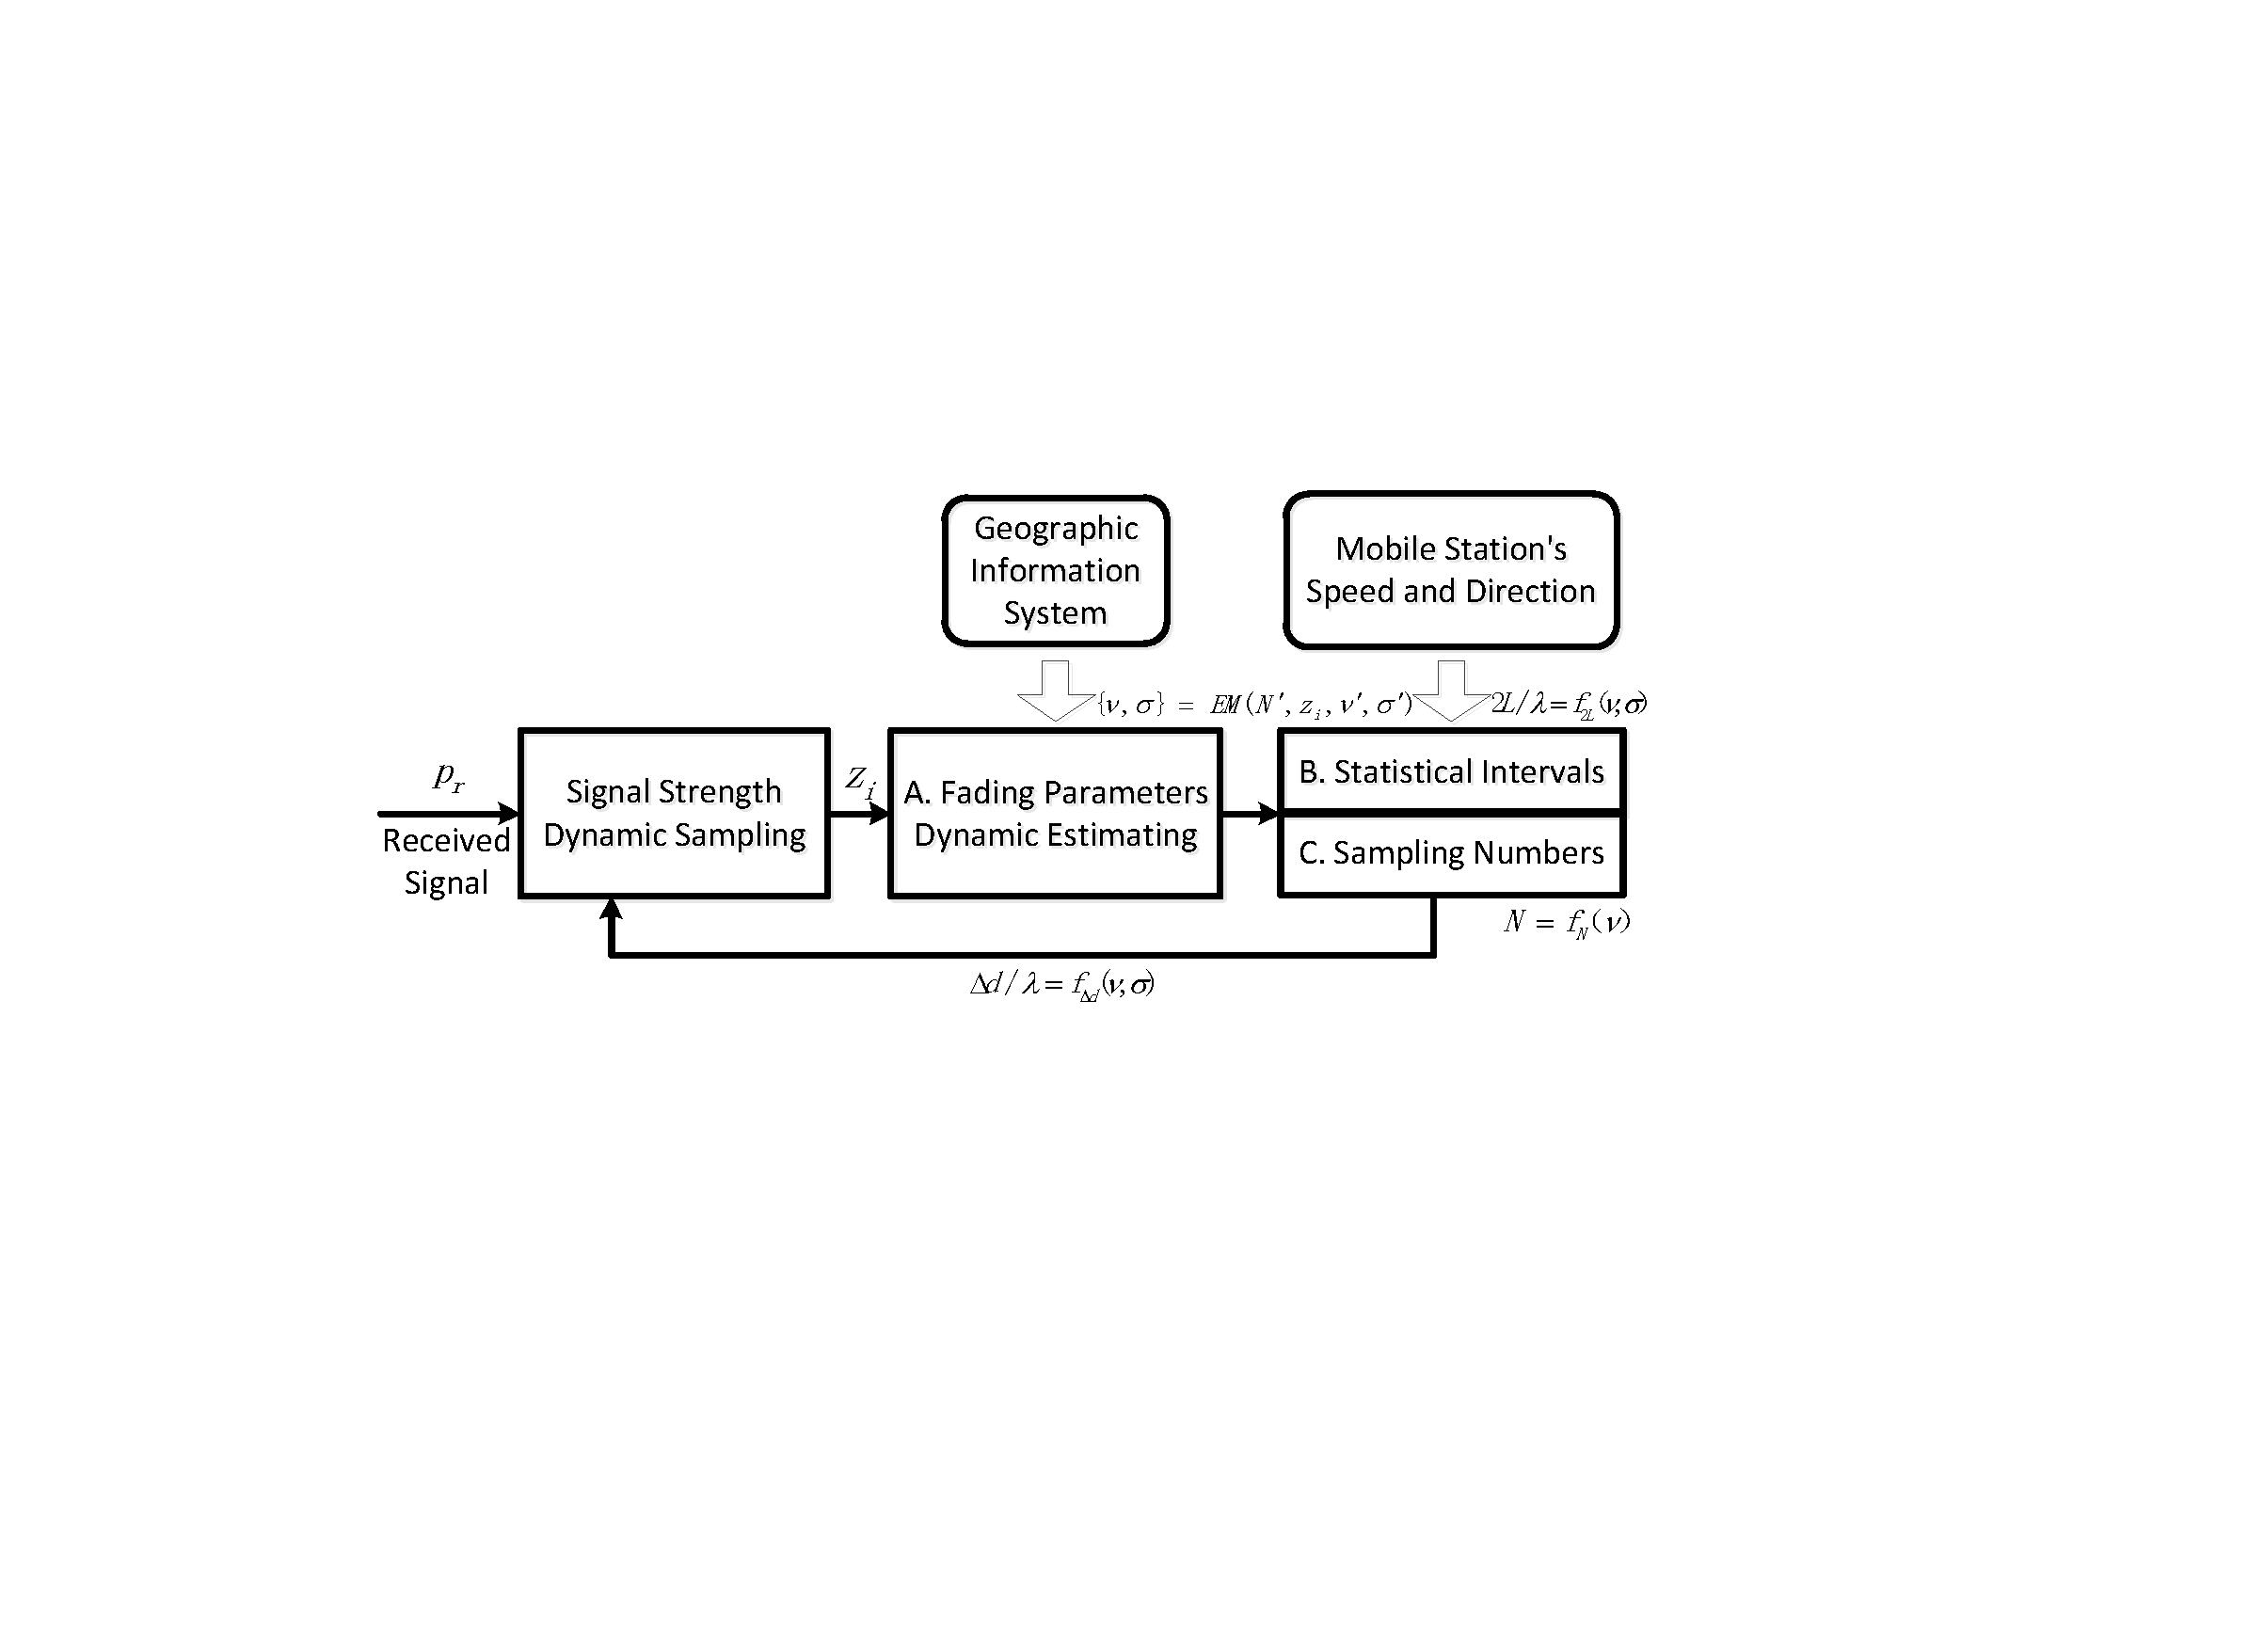
\includegraphics[width=5in]{chap2/online.pdf}
\bicaption[fig:online_measure]{在线动态测试框架}{在线动态测试框架}{Fig}{On-line and Dynamic Estimation of Rician Fading Channels}
\end{figure}

动态测试算法的工作过程如图 \ref{fig:online_measure} 所示,首先对信号进行动态采样,得到一组当前时刻的信号强度值,然后经过衰落参数动态估计,得到当前无线传播环境的莱斯衰落参数,然后经过计算得到统计区间与采样点数,同时以此为基础开始下一次信号采样。

\subsection{信道参数估计}
\label{sec:estimation}

对于莱斯衰落信道的参数估计已有大量相关工作,包括基于学习训练机制 \cite{bjornson2010framework}、最大似然估计 \cite{sijbers1998maximum} 以及期望最大化算法\cite{marzetta1995algorithm}。由于EM算法通过迭代方式进行参数估计,本文采用EM算法进行莱斯参数估计,以充分利用历史信息提高测试精度并降低测试开销。EM算法中莱斯衰落因子$\nu^2$和$\sigma^2$通过其上一时刻估计值与当前采样信号计算获得,如式(\ref{equa:EM})所示
\begin{subequations}
  \begin{eqnarray}
    \nu_{k+1}&=&\frac{1}{N}\sum_{i=1}^{N}\frac{I_{1}\left(\frac{\nu_{k}z_{i}}{\sigma_k^2}\right)}{I_{0}\left(\frac{\nu_{k}z_{i}}{\sigma_k^2}\right)}z_i \\
    \sigma_{k+1}^2&=&\max{\left[\frac{1}{2N}\sum_{i=1}^N z_i^2 -\frac{\nu_k^2}{2},0\right]}
  \end{eqnarray}
\label{equa:EM}
\end{subequations}
其中$I_1(\cdot)$一阶第一类修正贝塞尔函数,$N$为采样信号数码,$\nu_k$和$\sigma_k$为上一时刻估计结果,其初始值为
\begin{subequations}
  \begin{eqnarray}
    \nu_{0}&=& \left(2\left(\frac{1}{N}\sum_{i=1}^N z_i^2\right)^2-\frac{1}{N}\sum_{i=1}^N z_i^4\right)^{1/4} \\
    \sigma_{0}^2&=&\frac{1}{2}\left(\frac{1}{N}\sum_{i=1}^N z_i^2 - \nu_{0}\right)
  \end{eqnarray}
\label{equa:EM0}
\end{subequations}

基于以上的莱斯衰落参数估计,接收信号强度测试的采样频率可以计算得到,表示为信号波长$\lambda$与衰落参数$\nu$和$\sigma$的函数。采样频率$\Delta d$ 通过统计区间长度$2L$与采样点数目$N$的比值计算而来。

\subsection{统计区间长度}
\label{sec:length}

对于第 \ref{sec:channelmodel} 节的无线传播模型,接收信号强度的本地均值通过对采样信号$p_r(x)$在统计区间$2L$内进行积分平均获得,即
\begin{equation}
    \hat{s}=\frac{1}{2L}\int\limits_{y-L}^{y+L} p_r^2(x)dx=\frac{s}{2L}\int\limits_{y-L}^{y+L} h(x)dx
\label{equa:shadowmean}
\end{equation}

如果能够选取合适的统计区间长度$2L$,则估计值$\hat{s}$将逼近其实际值$s$,即$\hat{s}\rightarrow s$,此时小尺度衰落的均值表示为
\begin{equation}
\frac{1}{2L}\int\limits_{y-L}^{y+L} h(x)dx \rightarrow 1
\label{equa:shortterm}
\end{equation}

由式(\ref{equa:shadowmean})可知,估计值$\hat{s}$相对于真实值$s$的误差可以由$\hat{s}$的方差衡量,如式(\ref{equa:shadowvariance})所示
\begin{equation}
    \sigma_{\hat{s}}^{2}=\frac{1}{L}\int\limits_{0}^{2L}\left(1-\frac{\tau}{2L}\right)R_{p_{r}^2}(\tau)d\tau
\label{equa:shadowvariance}
\end{equation}
其中$R_{p_{r}^2}(\tau)=E[p_{r}^{2}(x)p_{r}^{2}(x+\tau)]-E[p_{r}^{2}(x)]E[p_{r}^{2}(x+\tau)]$为包络信号$p_{r}(x)$的自相关函数。则估计值$\hat{s}$的均一化误差可以表示为
\begin{equation}
P_e:=10 \log_{10}\left(\frac{\hat{s}+\sigma_{\hat{s}}}{\hat{s}-\sigma_{\hat{s}}}\right)
\label{equa:perror}
\end{equation}

将式(\ref{equa:shadowmean})和式(\ref{equa:shadowvariance})带入式(\ref{equa:perror})中,并按照附录\ref{appsec:lengthestimation}求解积分方程,归一化误差$P_e$可以表示为
\begin{equation}
P_e = 10 \log_{10}\left(\frac{\frac{2\sigma^2+\nu^2}{2\sigma^2}n+\sqrt{2(1+n)\int\limits_0^n g\left(\frac{\nu^2}{2\sigma^2};\rho\right) d\rho}}{\frac{2\sigma^2+\nu^2}{2\sigma^2}n-\sqrt{2(1+n)\int\limits_0^n g\left(\frac{\nu^2}{2\sigma^2};\rho\right) d\rho}}\right)
\label{equa:Perror}
\end{equation}
其中$\nu$和$\sigma$为莱斯衰落信道参数。令归一化误差等于1,即$P_e=1dB$,则可以得到合适的统计区间长度$2L$与信号波长$\lambda$及衰落参数$\nu^2$和$\sigma^2$的关系式,即$2L=f_{2L}(\lambda;\nu,\sigma)$或$2L/\lambda=f_{2L/\lambda}(\nu,\sigma)$,如图 \ref{fig:length} 所示。

\begin{figure}[!htp]
  \centering
  \subfigure[$\sigma=1$]{
    \label{fig:sigma1}
    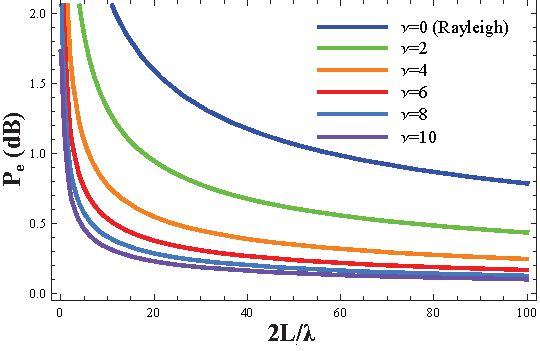
\includegraphics[width=2.5in]{chap2/sigma11.pdf}}
    \hspace{1cm}
  \subfigure[$\sigma=3$]{
    \label{fig:sigma3}
    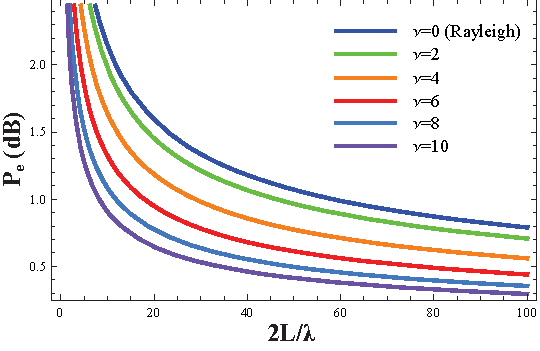
\includegraphics[width=2.5in]{chap2/sigma33.pdf}}
  \hspace{1in}
  \centering
  \subfigure[$\sigma=5$]{
    \label{fig:sigma5}
    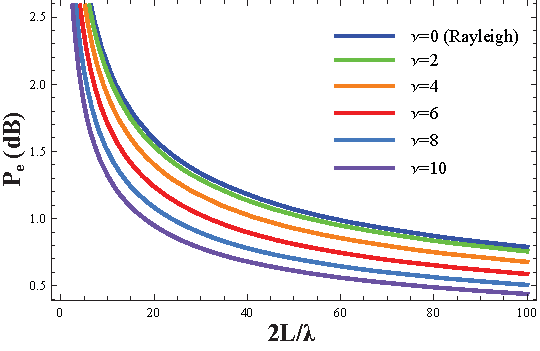
\includegraphics[width=2.5in]{chap2/sigma55.pdf}}
    \hspace{1cm}
  \subfigure[$\sigma=7$]{
    \label{fig:sigma7}
    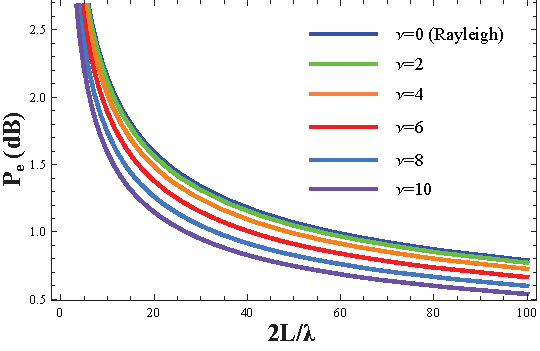
\includegraphics[width=2.5in]{chap2/sigma77.pdf}}
  \bicaption[fig:length]{统计区间长度}{统计区间长度}{Fig}{Proper Length of Statistical Intervals}
\end{figure}

\subsection{采样点数}
\label{sec:number}

除了选择合适的统计区间长度外,还需要确定采样点数目,以有效降低多径衰落对信号估计的影响。采样得到的接收信号功率可以通过衰落参数计算得到,结合式(\ref{equa:EM})有$r^2=2\sigma^2+\nu^2\approx\frac{1}{N}\sum_{i=1}^N z_i^2$,则$r^2$的估计值及其方差为
\begin{subequations}
  \begin{eqnarray}
    \bar{r^2}&=&E\left[r^2\right]=\frac{1}{N}E\left[\sum_{i=1}^{N}z_i^2\right] \\
    \sigma_{\bar{r^2}}&=&D\left[r^2\right]=\frac{1}{N^2}D\left[\sum_{i=1}^{N}z_i^2\right]
  \end{eqnarray}
\label{equa:number}
\end{subequations}

与统计区间长度的归一化误差类似,采样点数目的归一化误差为
\begin{equation}
Q_e=10 \log_{10}\left(\frac{\bar{r^2}+\sigma_{\bar{r^2}}}{\bar{r^2}}\right)
\label{equa:qerror}
\end{equation}

根据附录 \ref{appsec:numberestimation} 中的计算与推导,$Q_e$可以表示为
\begin{equation}
    Q_e=10 \log_{10}\left(\frac{2N+\nu^2+2\sqrt{N+\nu^2}}{2N+\nu^2}\right)
\label{equa:Qerror}
\end{equation}
其中$\nu$和$\sigma$为莱斯衰落参数,通过如式(\ref{equa:EM})中EM算法计算得到。显然采样点数目只与莱斯衰落参数$\nu$有关,即$N=f_{N}(\nu)$,如图 \ref{fig:nu} 所示。

\begin{figure}[!htp]
\centerline{
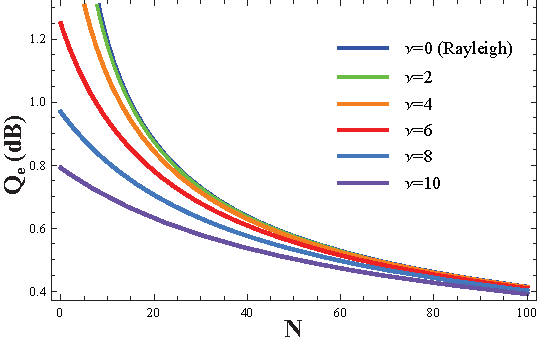
\includegraphics[width=4.0in]{chap2/nu1.pdf}
}
\bicaption[fig:nu]{采样点数}{采样点数}{Fig}{Required Number of Averaging Samples}
\end{figure}

接收信号强度采样频率$\Delta d$由$2L/N$计算获得,即$\Delta d=f_{2L}(\lambda;\nu,\sigma)/f_{N}(\nu)=f_{\Delta d}(\lambda;\nu,\sigma)$。 由于信号波长$\lambda$在通信过程中一般保持不变,因此$\Delta d$与莱斯衰落参数$\nu$和$\sigma$密切相关。

\section{系统实现}
\label{sec:system_phy}

GSM-R网络通信质量测试系统主要完成物理指标的实时测量,同时对网络链路质量进行统计与分析,包括实时测试与离线分析。GSM-R网络空中接口测试系统实现对GSM-R网络通信质量的在线实时与离线综合测试,如图 \ref{fig:umsystem} 所示。在线测试实现对GSM-R网络通信质量的实时监测,同时在网络出现故障时给出预警信息;离线测试对GSM-R网络性能进行统计与分析,给出网络的综合性能评估,并提出参数调整建议。同时测试指标包含网络物理层、链路层与业务层各项指标,实现对GSM-R网络通信质量的全面测试,保证高铁系统的安全稳定高速运行。

\begin{figure}[!htp]
%\onelinecaptionsfalse
\centering
    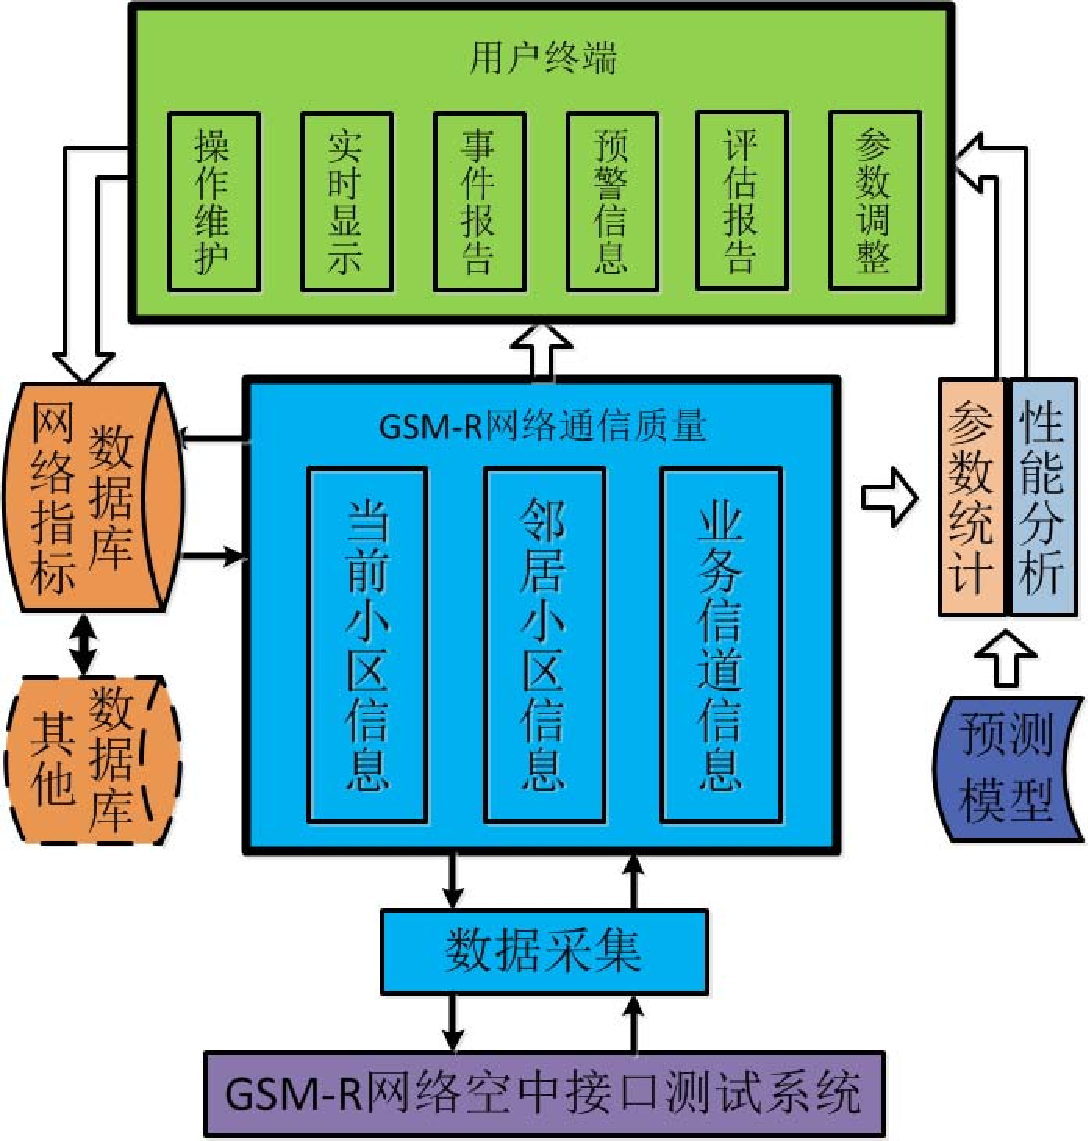
\includegraphics[width=5in]{chap2/softwarefunction.pdf}
\bicaption[fig:umsystem]{GSM-R网络空中接口测试系统}{GSM-R网络空中接口测试系统}{Fig}{Um interface monitoring system for GSM-R networks}
\end{figure}

本章首先引入GSM-R网络空中接口测试系统的基本结构,包括硬件平台与软件开发,然后分析动态测试算法的设计与实现,最后对系统的基本功能进行简单介绍。

\subsection{硬件平台}
\label{sec:um}

GSM-R网络测试系统由无线收发模块、通信协议处理模块、数据分析处理模块构成,如图 \ref{fig:umhardware} 所示,其中无线收发模块完成GSM-R网络通信信号采集,通信协议处理模块主要对采集到的网络信令进行解析,数据分析处理模块负责对网络各项性能指标进行统计与分析。

\begin{figure}[!htp]
%\onelinecaptionsfalse
\centering
    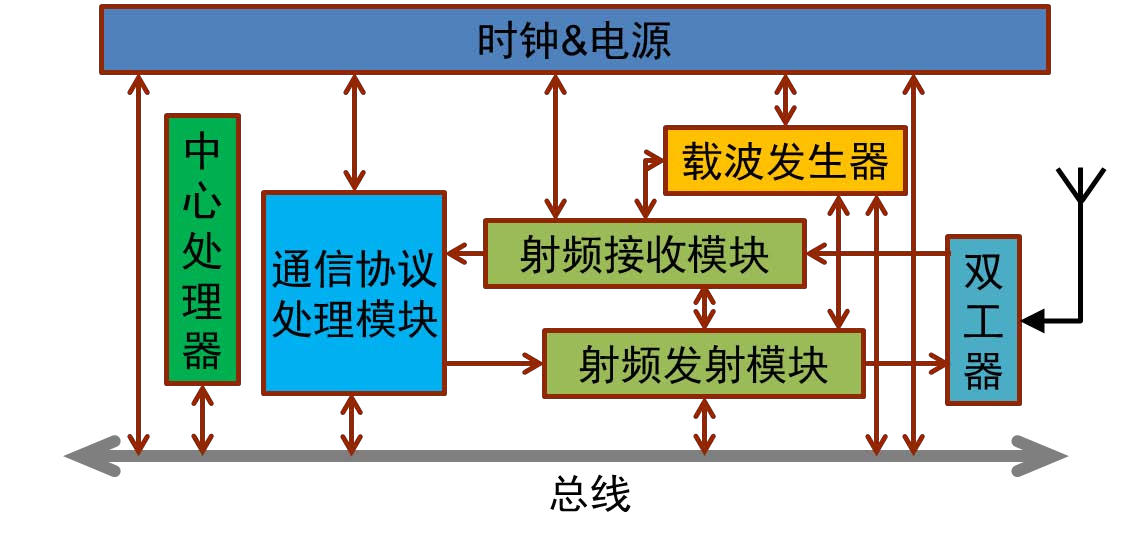
\includegraphics[width=5in]{chap2/hardware.pdf}
\bicaption[fig:umhardware]{GSM-R网络空中接口测试系统硬件组成}{GSM-R网络空中接口测试系统硬件组成}{Fig}{Hardware components of Um interface monitoring system for GSM-R networks}
\end{figure}

测试系统中心处理器模块为美国RTD公司的CME137686LX-W cpuModules™,通信协议处理模块与射频收发模块选择德国Triorail公司的GSM-R网络收发模块TRM:3a,外加RTD公司的GSM-R网络收发模块外围开发板COM16155RER-1,上述模块通过PC/104与RTD的电源模块VPWR104HR-L50W相连接,从而实现GSM-R 网络信息收发功能。

GSM-R网络空中接口测试系统的硬件平台由PC/104总线实现模块间通信,主要由以下三部分组成:
\begin{itemize}
  \item \textbf{处理器模块}
  处理器模块采用RTD公司符合军工标准的CME137686LX-W模块,该模块采用500MHz AMD™ Geode LX处理器,具有128kB L1缓存和128kB L2缓存,采用333MHz DDR-SDRAM控制器支持最高2.7G-Bytes/s的存储带宽,包括4个USB 2.0 接口, 2个SATA II 接口, 3个串口、千兆以太网口、8GB板贴固态硬盘和8个GPIO,在有效完成数据处理的同时,满足高速铁路复杂的无线传播环境。
  \item \textbf{无线通信模块}
  COM16155ER模块板载Cinterion 4频段GSM/GPRS模块MC55i和Fastrax IT500 GPS模块,在实际测试过程中,将GSM模块替换为德国Triorail公司的GSM-R收发模块TRM:3a。COM16155ER板载两个ISA总线接口的UART,分别连接到GSM-R模块和GPS模块,主机模块通过UART和相关接口对GSM-R模块和GPS模块进行操作。
  \item\textbf{电源模块}
  电源模块采用RTD的电源模块VPWR104HR-L50W,输入电压20-28VDC,输出电压-12V到+19V,工作温度-40到+85C$\circ$,能够满足高速铁路的特殊环境要求。
\end{itemize}

上述各模块符合工业级标准,性能稳定并能够工作在各种恶劣环境,同时PC/104作为工业级总线能够保证系统的实时性与可靠性。

\subsection{软件开发}
\label{sec:softwaregsmmr}

GSM-R网络空中接口测试软件平台的开发基于Visual Studio 2008开发环境,开发语言为C\#,软件运行平台为Windows XP、Windows Mobile或Windows CE 操作系统,运行环境Microsoft .NET Compact Framework 2.0或者以上版本,测试系统的启动和运行界面如图 \ref{fig:copyright} 和图 \ref{fig:interface} 所示。

\begin{figure}[!htp]
%\onelinecaptionsfalse
\centering
    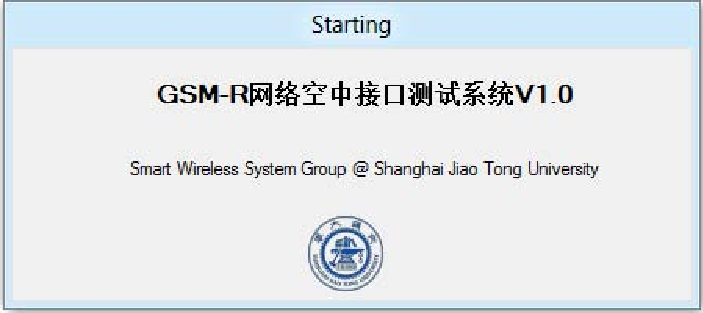
\includegraphics[width=3in]{chap2/softwarecopyright.pdf}
\bicaption[fig:copyright]{GSM-R网络空中接口测试系统启动界面}{GSM-R网络空中接口测试系统启动界面}{Fig}{Software starting of Um interface monitoring system for GSM-R networks}
\end{figure}

\begin{figure}[!htp]
%\onelinecaptionsfalse
\centering
    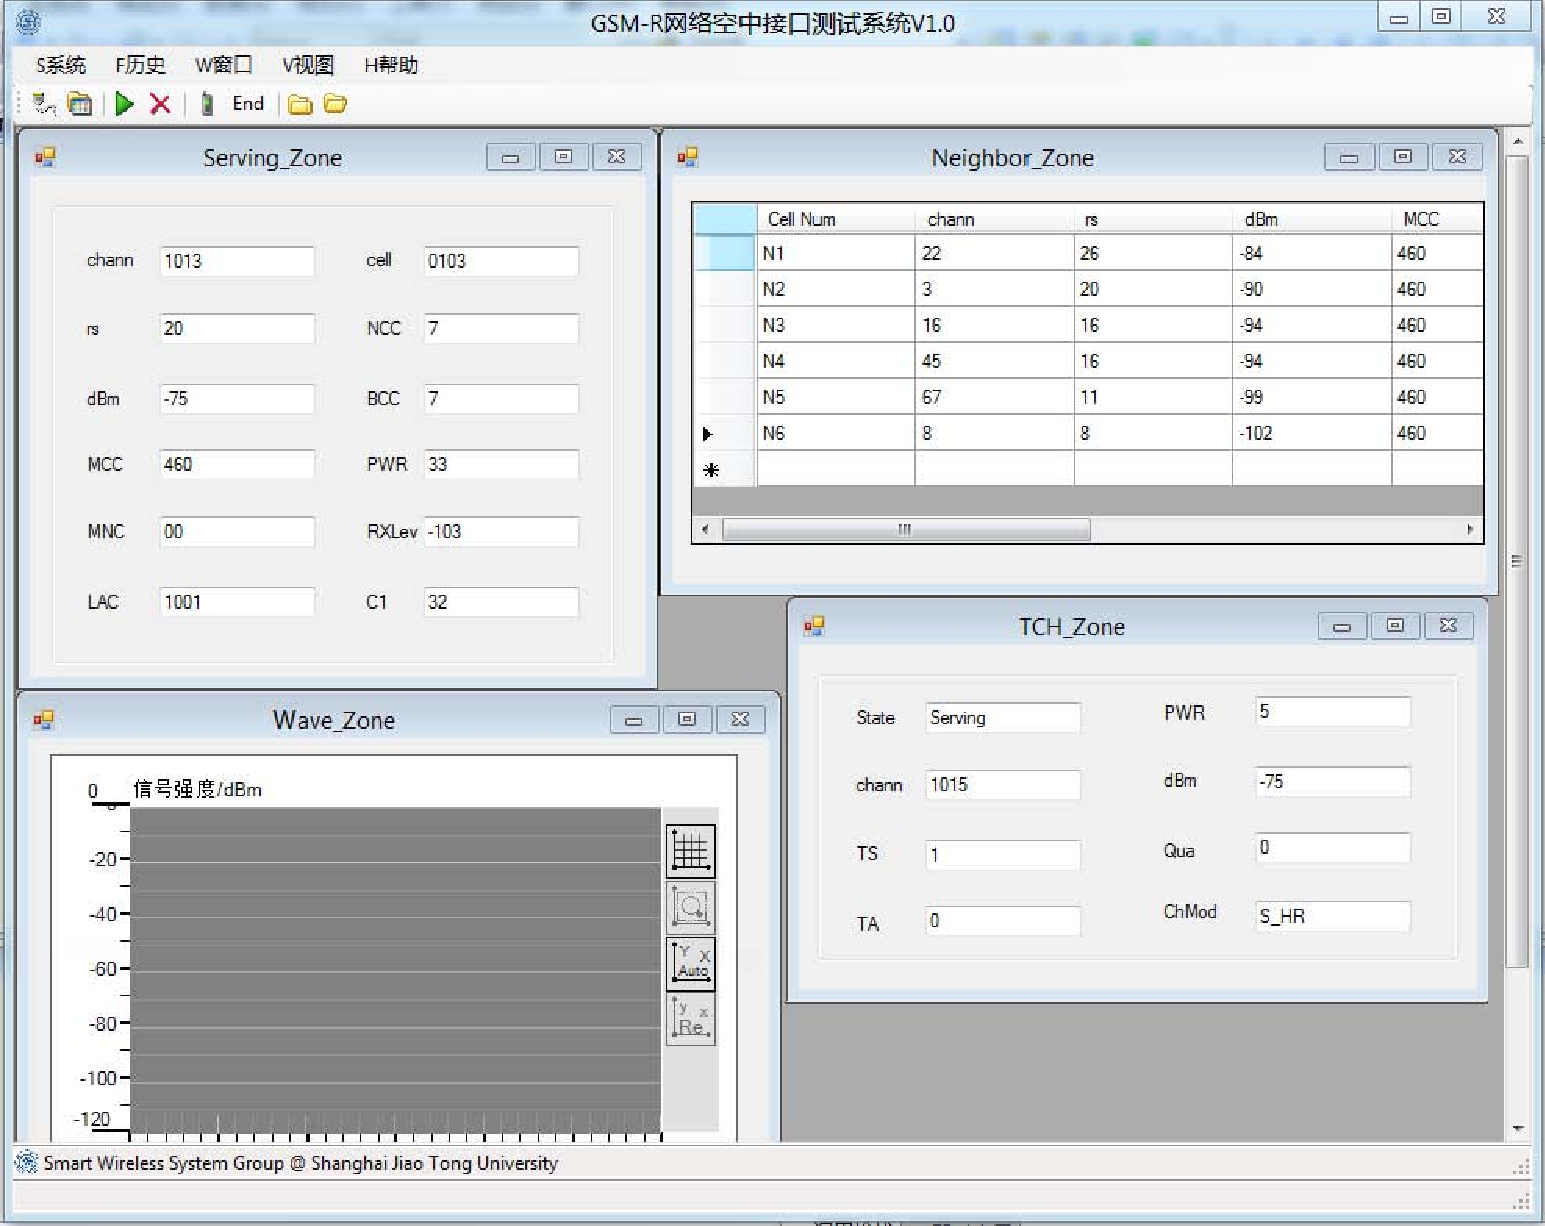
\includegraphics[width=4.5in]{chap2/softwarestart.pdf}
\bicaption[fig:interface]{GSM-R网络空中接口测试系统软件界面}{GSM-R网络空中接口测试系统软件界面}{Fig}{Software interface of Um interface monitoring system for GSM-R networks}
\end{figure}

\subsection{算法实现}
\label{sec:alggsmr}

GSM-R网络接收信号强度在线测试的伪代码如算法 \ref{alg:online} 所示,主要基于第 \ref{sec:dynamic} 章的推导与计算。首先通过EM算法进行莱斯衰落参数估计,实现莱斯衰落因子$\nu_0$和$\sigma_0$的初始化,此时的信号采样参数去瑞利衰落时的参数设置,即统计区间$2L=40\lambda$,采样点数$N=36$。然后在每一轮采样周期基于上一轮估计结果和当前采样信息,对衰落因子$\nu_k$和$\sigma_k$进行实时更新,同时确定下一轮采样参数$2L$和$N$。最后通过统计区间长度和采样点数计算得到采样间隔$\Delta d=2L/N$,并开始新一轮的信号采样与参数估计。

\begin{figure}[!htp]
%\onelinecaptionsfalse
\centering
    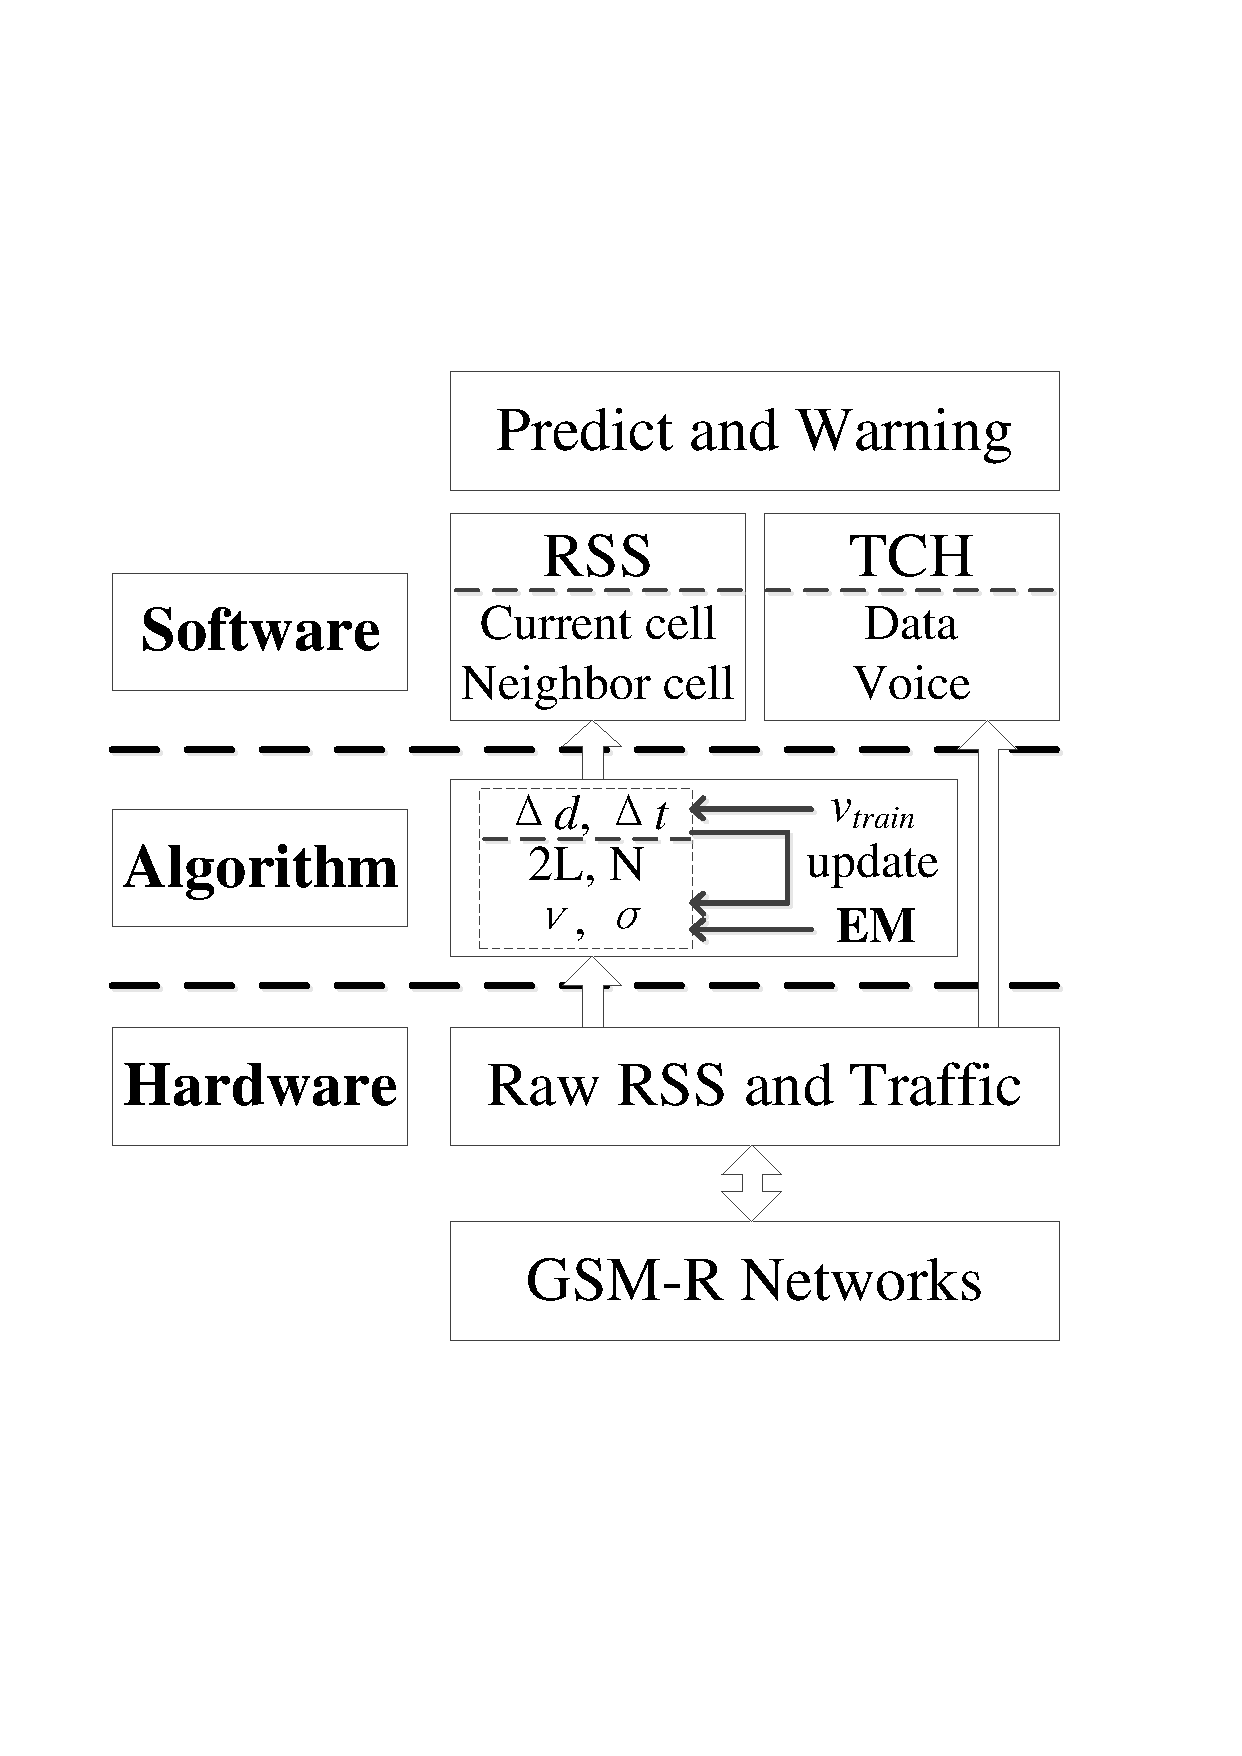
\includegraphics[width=3.6in]{chap2/umframework.pdf}
\bicaption[fig:umframework]{信道状态估计算法与实现}{信道状态估计算法与实现}{Fig}{Estimation framework and algorithm implementation}
\end{figure}

GSM-R网络信道动态测试为上层应用提供准确的网络状态信息,如图 \ref{fig:umframework} 所示,测试系统首先通过GSM-R收发模块,获得接收信号强度的原始信息;然后由动态采样算法进行数据处理与参数估计,并提供当前网络状态信息,包括物理层信道状态与链路质量信息;同时系统根据历史信息对网络状态进行预测,在信号强度持续下降时给出预警信息;最后动态测试算法将所有原始数据及网络状态信息提供给软件界面及数据库,用于显示当前网络状态信息,或进行网络性能的分析与评估,包括切换性能分析与网络优化。

\begin{algorithm}[!htp]
\floatname{algorithm}{算法}
\renewcommand{\algorithmicrequire}{\textbf{输入:}}
\renewcommand{\algorithmicensure}{\textbf{输出:}}
\caption{莱斯衰落信道在线采样与估计}
\label{alg:online}
\begin{algorithmic}[1]
\Require $v_{train}$, $r_i$, $\nu_k$, $\sigma_k$
\Ensure  $\nu_{k+1}$, $\sigma_{k+1}$, $2L$, $N$, $\Delta d$
\State {// 1. 衰落参数$\nu$和$\sigma$初始化}
\If {begin-flag==true}
\State {$\Delta d$ $\leftarrow$ Lee($2L_0$,$N_0$;$\lambda$);}
\State {\{$\nu_{last}$, $\sigma_{last}$\} $\leftarrow$ EM($\Delta d$,$N_0$;$r_i$); // 式(\ref{equa:EM0})}
\State {\{$\nu_{now}$, $\sigma_{now}$\} $\leftarrow$ EM($\Delta d$,$N_0$;$r_i$;$\nu_{last}$,$\sigma_{last}$); // 式(\ref{equa:EM})}
\While {($\nu_{now}-\nu_{last}>\nu_{thr}$) \& ($\sigma_{now}-\sigma_{last}>\sigma_{thr}$)}
\State {\{$\nu_{next}$, $\sigma_{next}$\} $\leftarrow$ EM($\Delta d$,$N_0$;$r_i$;$\nu_{now}$,$\sigma_{now}$); // 式(\ref{equa:EM})}
\State {$\{\nu_{last},\sigma_{last}\} \leftarrow \{\nu_{now},\sigma_{now}\}$;}
\State {$\{\nu_{now},\sigma_{now}\} \leftarrow \{\nu_{next},\sigma_{next}\}$;}
\EndWhile
\State {$2L_{now} \leftarrow f_{2L}(\lambda;,\nu_{now},\sigma_{now})$; // 式(\ref{equa:Perror})}
\State {$N_{now} \leftarrow f_{N}(\nu_{now})$; // 式(\ref{equa:Qerror})}
\EndIf
\State {// 2. $\nu$和$\sigma$实时估计,计算采样参数$2L$、$N$和$\Delta d$.}
\If {operating-flag==true}
\For {$i=0;i<N_{now};i++$}
\State {\{$\nu_{next}$, $\sigma_{next}$\} $\leftarrow$ EM($\Delta d$,$N_0$;$r_i$;$\nu_{now}$,$\sigma_{now}$); // 式(\ref{equa:EM})}
\State {$2L_{next} \leftarrow f_{2L}(\lambda;,\nu_{now},\sigma_{now})$; // 式(\ref{equa:Perror})}
\State {$N_{next} \leftarrow f_{N}(\nu_{now})$; // 式(\ref{equa:Qerror})}
\State {$\Delta d_{next} = f_{2L}(\lambda;,\nu_{now},\sigma_{now})/f_{N}(\nu_{now})$;}
\State {$\{\nu_{last},\sigma_{last};2L_{last},N_{last}\} \leftarrow \{\nu_{now},\sigma_{now};2L_{now},N_{now}\}$;}
\State {$\{\nu_{now},\sigma_{now};2L_{now},N_{now}\} \leftarrow \{\nu_{next},\sigma_{next};2L_{next},N_{next}\}$;}
\If {$i==N_{last}$}
\State {i=0;}
\EndIf
\EndFor
\EndIf
\end{algorithmic}
\end{algorithm}

\subsection{基本功能}
\label{sec:function}

GSM-R网络空中接口测试系统的基本功能如图 \ref{fig:umsoftwarefunc} 所示,主要完成网络通信质量的测试、处理、预测、显示与预警。

\begin{figure}[!htp]
%\onelinecaptionsfalse
\centering
    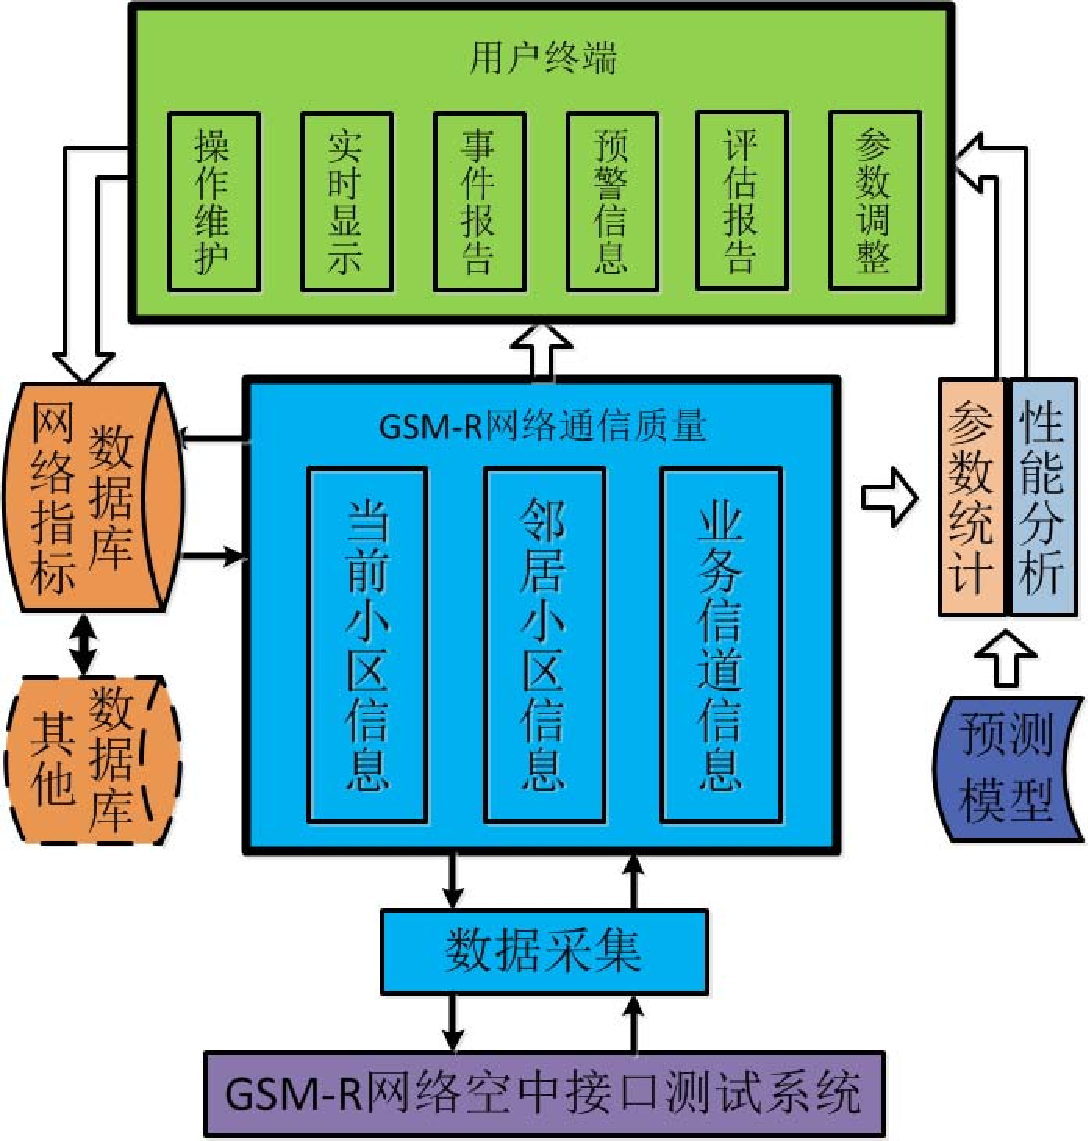
\includegraphics[width=4in]{chap2/function.pdf}
\bicaption[fig:umsoftwarefunc]{GSM-R网络空中接口测试系统软件结构}{GSM-R网络空中接口测试系统软件结构}{Fig}{Software architecture of Um interface monitoring system for GSM-R networks}
\end{figure}

测试系统在硬件配置完成后,测试软件首先对GSM-R网络空中接口传输的信息进行解析,得到网络当前时刻与位置的通信质量信息,并根据GSM-R网络当前小区信息得到网络当前广播控制信道、语音业务信道和数据域业务信道质量信息,并给出小区切换和信道切换的分布图,同时绘制当前服务小区广播控制信道的接收信号强度和邻居小区广播控制信道接收信号质量的曲线轨迹,利用当前测试数据与历史数据,结合预测模型对网络的无线传播进行预测,在当前网络通信质量低于系统要求时给出警告信息,结合地理信息和基站信息,给出测试报告并对GSM-R网络性能进行整体评估。
\begin{itemize}
  \item 当前小区信息:显示移动台当前所在小区基本信息,包括小区编号、信道编号、接收信号强度、基站识别码、功率等级和小区重选系数等信息。
  \item 邻居小区信息:显示接收信号强度最好的三个到六个邻居小区的信息,包括信道编号、接收信号强度、基站识别码和小区重选系数等。
  \item 业务信道信息:显示当前业务信道基本信息,包括信道编号、时隙分配、时间提前量、功率大小、接收信号强度、接收信号质量和信道模式等。
  \item 曲线绘制:实时记录当前小区及邻居小区的接收信号强度信息,并能够调取历史数据和数据库中的数据,进行场景重现。
  \item 历史数据:导入或导出历史数据,实现对任意时刻的通信情况进行分析,为GSM-R网络的优化提供数据支持。
\end{itemize}

\begin{figure}[!htp]
%\onelinecaptionsfalse
\centering
    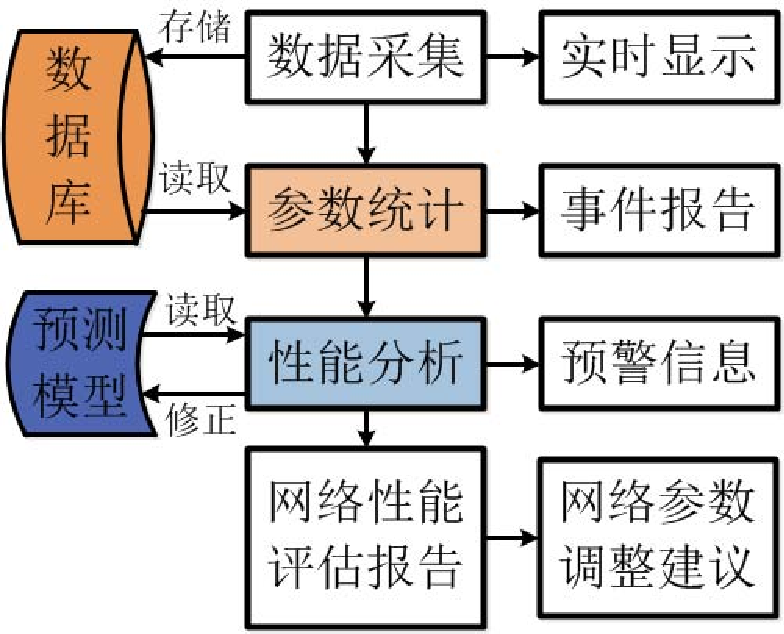
\includegraphics[width=3in]{chap2/dataprocess.pdf}
\bicaption[fig:umprocess]{GSM-R网络空中接口测试系统数据处理}{GSM-R网络空中接口测试系统数据处理}{Fig}{Data processing of Um interface monitoring system for GSM-R networks}
\end{figure}


\section{性能评估}
\label{chap:evaluation_phy}

本节主要介绍动态测试算法的实验分析与性能评估,通过GSM-R网络空中接口测试系统,由高速列车上的移动终端在京沪高速铁路沿线进行接收信号强度信息采集,如图 \ref{fig:platform} 所示。

\begin{figure}[!htp]
\centering
\subfigure[硬件平台]{
    \label{fig:hardware}
    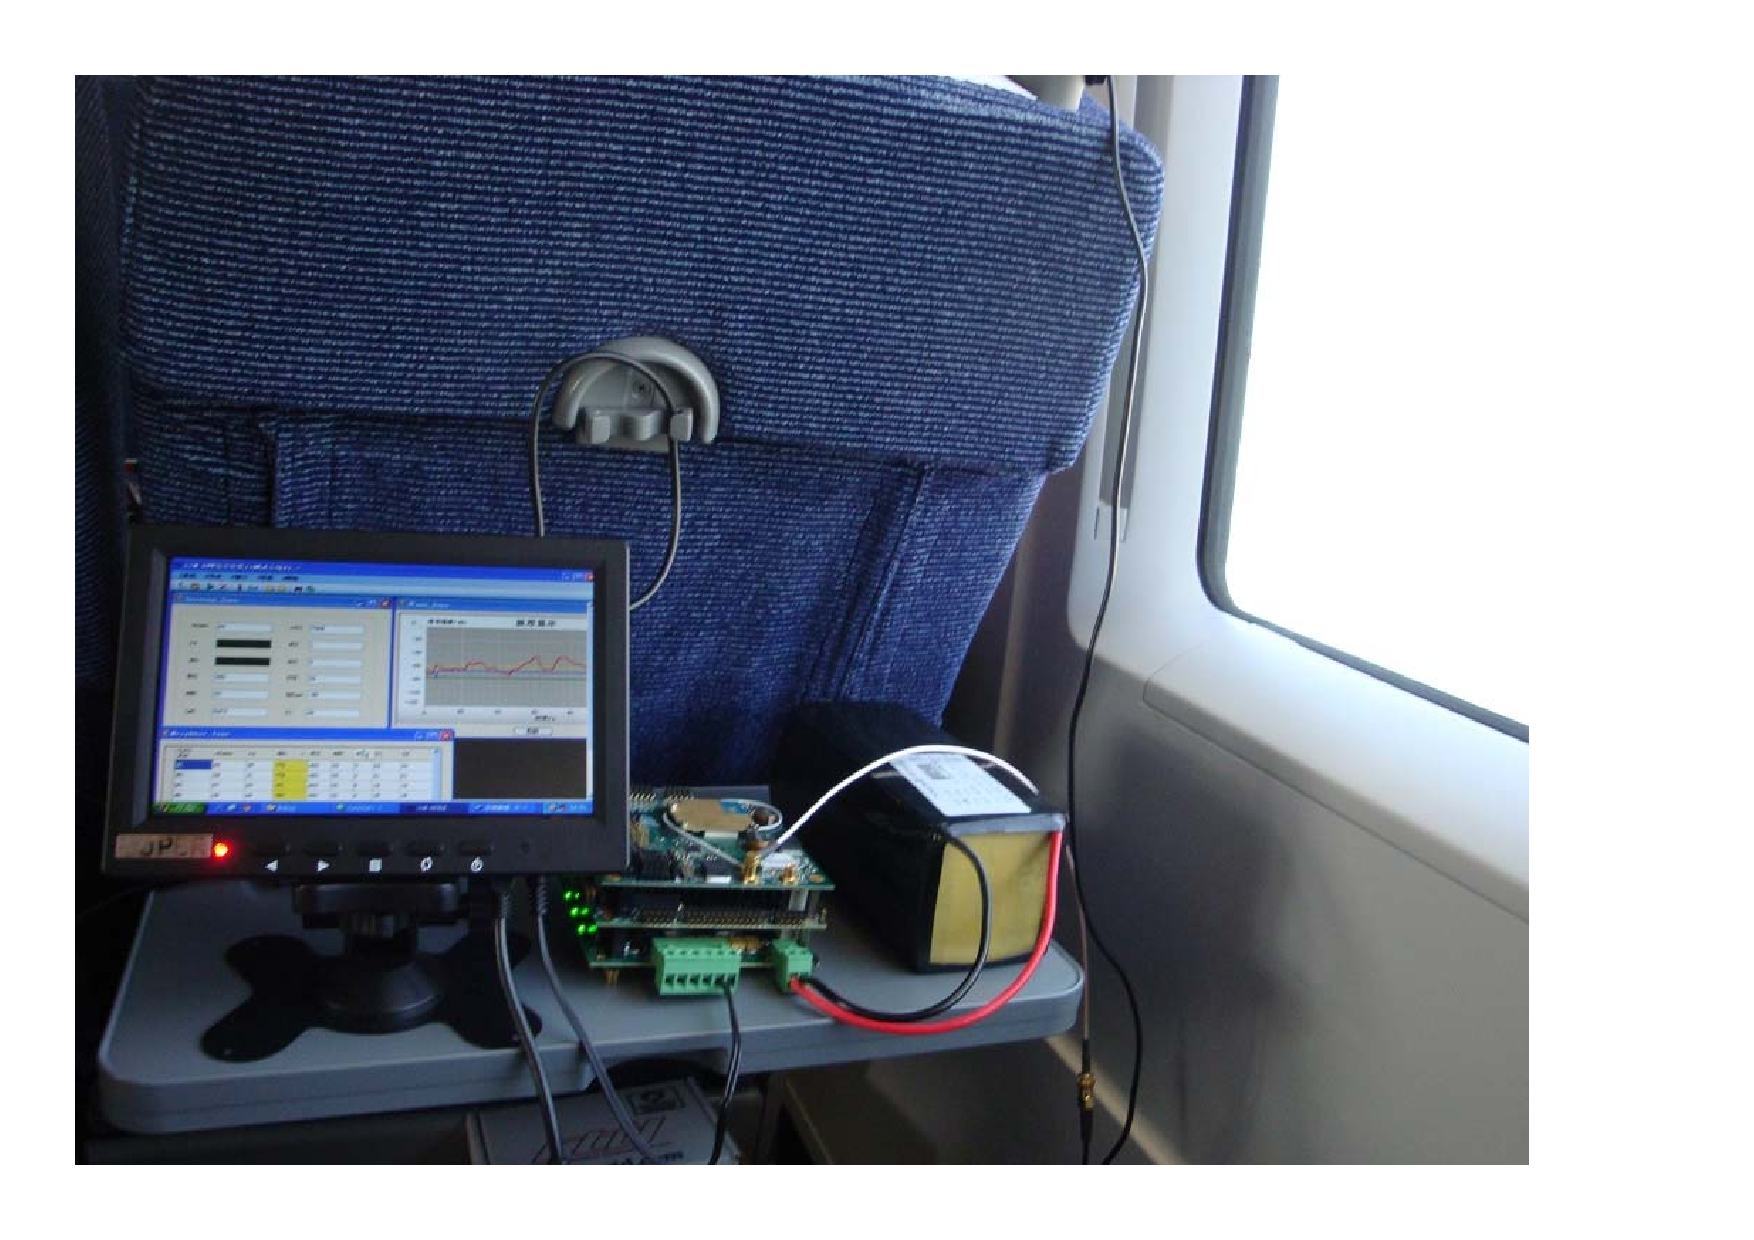
\includegraphics[width=2.5in]{chap2/platform.pdf}}
    \hspace{1cm}
\subfigure[软件平台]{
    \label{fig:software}
    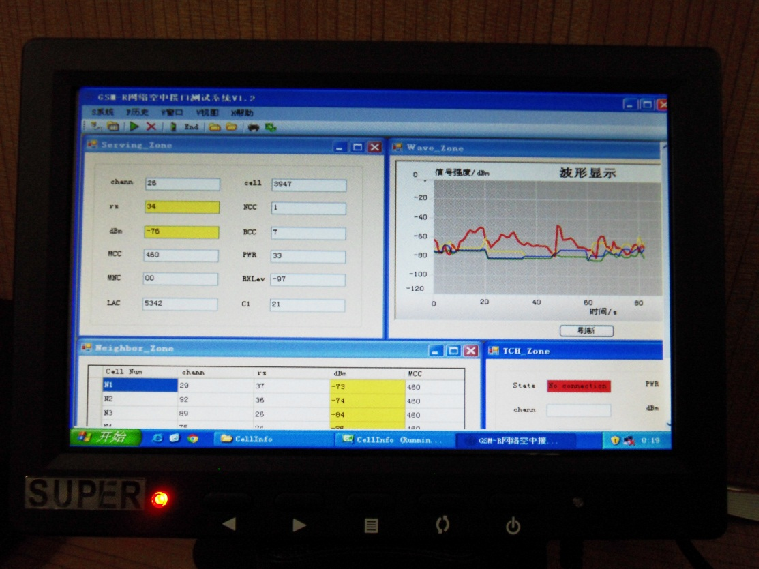
\includegraphics[width=2.5in]{chap2/softwareinterface.pdf}}
\bicaption[fig:platform]{GSM-R网络空中接口测试系统}{GSM-R网络空中接口测试系统}{Fig}{Um Interface Monitoring System for GSM-R Networks}
\end{figure}

实验测试结果以XML格式进行存储与处理,如图 \ref{fig:xml} 所示为京沪高铁GSM-R网络接收信号强度信息。动态估计算法的测试结果如表 \ref{tab:summary} 所示,包括不同无线传播环境下的莱斯衰落参数与采样参数,其中无线传播类型由莱斯衰落参数$K$表示:当$K=0$时表示没有直射路径信号,此时莱斯衰落退化为瑞利衰落;当$K$逐步增加表示无线传播环境逐渐平坦。

\begin{figure}[!htp]
\centering
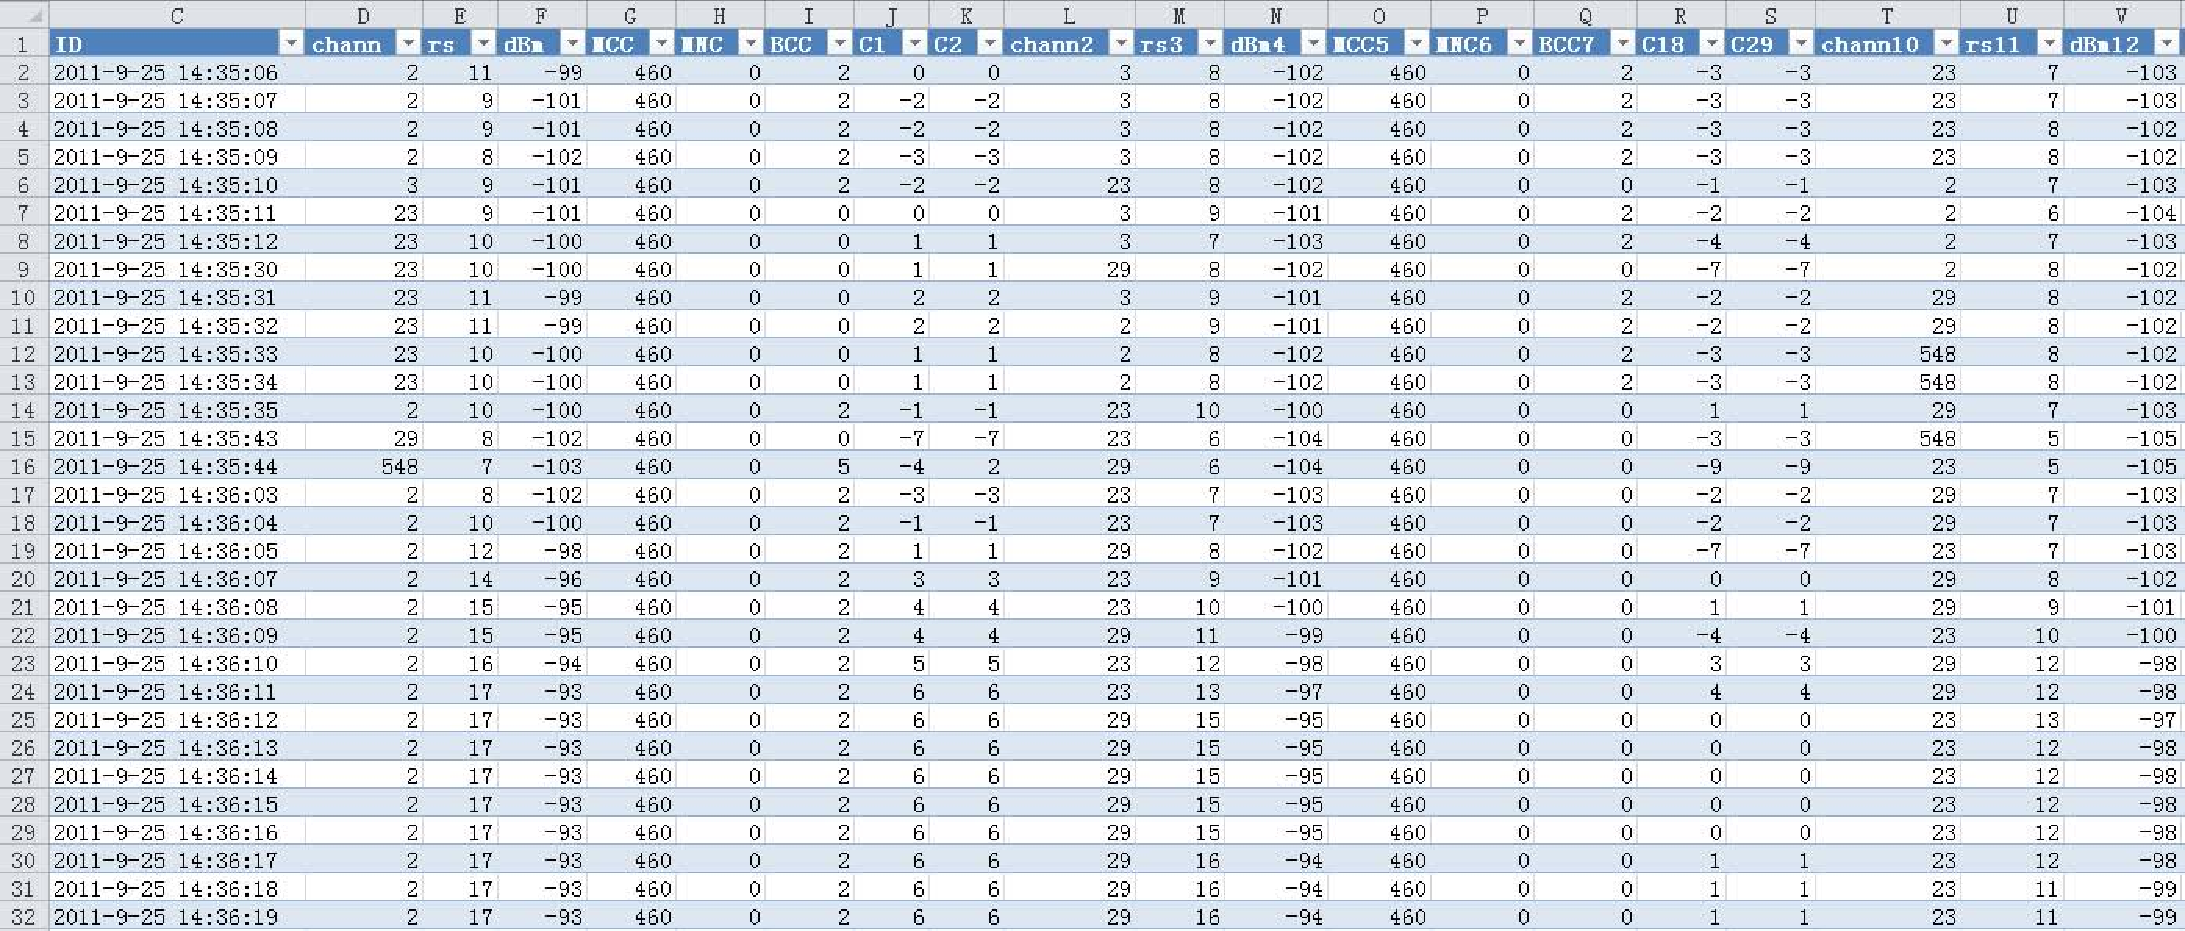
\includegraphics[width=1\textwidth]{chap2/xml.pdf}
\bicaption[fig:xml]{信道状态测试结果}{信道状态测试结果}{Fig}{Measurement Results}
\end{figure}

从表 \ref{tab:summary} 中的数据可以看出,在莱斯因子$K = 0$时,统计区间为$2L = 40\lambda$,采样间隔为$\Delta d = 0.5\lambda$;随着莱斯因子$K$的增大,无线传播环境逐渐平坦,导致直射路径功率比例增加,统计区间与采样间隔逐渐降低;当$\nu \geq 8$时所需的采样点数$N \leq 10$,即在不同统计区间内只需做$N \leq 10$次采样,便可以保证本地均值的准确性,同时在$K$值逐渐增大过程中,统计区间相应增大,且不需要做频繁的数据采集,采样间隔在$1m$左右。

\begin{table}[!htp]
\renewcommand{\arraystretch}{1}
\bicaption[tab:summary]{信道状态估计结果总结}{信道状态估计结果总结}{Table}{Summary of Experiment Results of Channel State Estimation}
\centering
\begin{threeparttable}[b]
\begin{tabular}{c|c|c|c|c|c|c|c|c|c|c}
%\toprule
\hline
%\cline{1-11}
\multicolumn{1}{c|}{\multirow{3}{*}{Terrain}} & \multicolumn{1}{c|}{\multirow{3}{*}{$K$(dB)}} & \multicolumn{1}{c|}{\multirow{3}{*}{$\nu$}} & \multicolumn{1}{c|}{\multirow{3}{*}{$\sigma$}} & \multicolumn{1}{c|}{\multirow{3}{*}{$2L/\lambda$}} & \multicolumn{1}{c|}{\multirow{3}{*}{$N$}} & \multicolumn{1}{c|}{\multirow{3}{*}{$\Delta d/\lambda$}} & \multicolumn{1}{c|}{\multirow{3}{*}{$\Delta d$(m)}} & \multicolumn{3}{c}{$v_{train}$(km/h)}\\
\cline{9-11}
\multicolumn{1}{c|}{} & \multicolumn{1}{c|}{} & \multicolumn{1}{c|}{} & \multicolumn{1}{c|}{} & \multicolumn{1}{c|}{} & \multicolumn{1}{c|}{} & \multicolumn{1}{c|}{} & \multicolumn{1}{c|}{} & 200 & 250 & 300\\
\cline{9-11}
\multicolumn{1}{c|}{}& \multicolumn{1}{c|}{} & \multicolumn{1}{c|}{} & \multicolumn{1}{c|}{} & \multicolumn{1}{c|}{} & \multicolumn{1}{c|}{} & \multicolumn{1}{c|}{} & \multicolumn{1}{c|}{} & \multicolumn{3}{c}{$\Delta t$(ms)}\\
%\midrule[5pt]
%\hline
%\hline
\cline{1-11}
NLOS\tnote{*}  &  0 &    - & - & 40 & 36 &  1.1 & 0.367 &  2.20 &  1.76 &  1.47\\
\hline
Dense &  0 &   0 & 1 & 55 & 15 &  3.7 & 1.222 &  7.33 &  5.86 &  4.89\\
      &  2 &   4 & 2 & 18 & 12 &  1.5 & 0.500 &  3.00 &  2.40 &  2.00\\
      &  4 & 5.6 & 2 &  9 &  9 &  1.0 & 0.333 &  2.00 &  1.60 &  1.33\\
      &  6 &   6 & 3 & 20 &  7 &  2.9 & 0.967 &  5.80 &  4.64 &  3.87\\
      &  8 &  12 & 3 &  8 &  1 &  8.0 & 2.667 & 16.00 & 12.80 & 10.67\\
Open  & 10 &  18 & 4 & 12 &  1 & 12.0 & 4.000 & 24.00 & 19.20 & 16.00\\
%\bottomrule[10pt]
\hline
%\cline{1-11}
\end{tabular}
\begin{tablenotes}
\item[*] \small Caculated by Lee's method of local mean power estimation in the case of Rayleigh fading
\end{tablenotes}
\end{threeparttable}
\end{table}

\begin{figure}[!htp]
\centering
    \subfigure[接收信号强度与大尺度衰落]{
    \label{fig:input}
    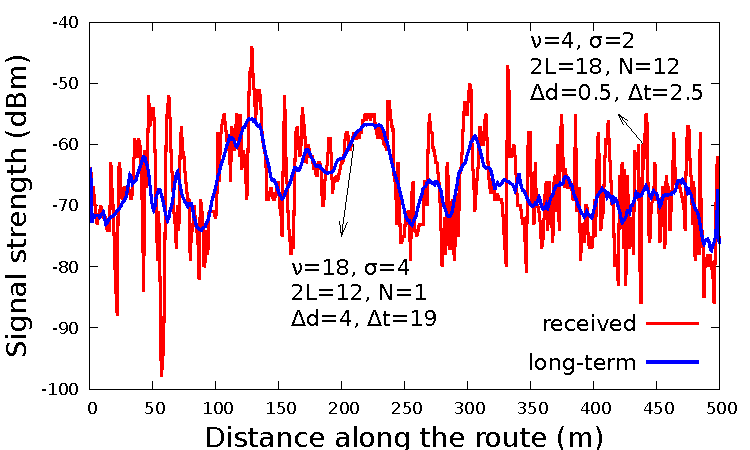
\includegraphics[width=4.5in]{chap2/em.pdf}}
\hspace{1in}
\centering
    \subfigure[小尺度衰落]{
    \label{fig:output}
    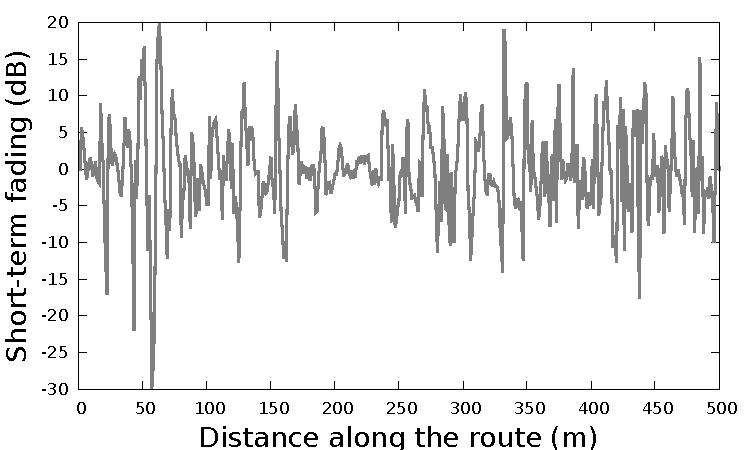
\includegraphics[width=4.5in]{chap2/short.pdf}}
\bicaption[fig:strength]{接收信号强度与信号衰落}{接收信号强度与信号衰落}{Fig}{Received signal strength and signal fading}
\end{figure}

对于运行于900MHz的GSM-R网络而言,Lee氏采样算法的采样间隔为$36cm$,工程应用中采用每隔$4cm$的采样方式,在相同的测试精度的前提下,即保证归一化误差为1dB,动态采样算法能够实现测试误差的显著降低,从而在完成通信性能测试的同时保证网络的正常通信。

通过动态测试算法获得的接收信号强度信息如图 \ref{fig:strength} 所示,大尺度和小尺度衰落经过动态测试算法能够有效区分,从而能够进行分别分析与处理。大尺度衰落通过最大似然估计或最小均方差估计,实现无线传播预测或模型修正;小尺度衰落对于无线网络的切换算法、功率控制及频谱分配等具有重要影响,例如切换算法中切换门限的选择与设置。

\section{本章小结}
\label{sec:conclusion2}

本章讨论了在莱斯衰落环境下,GSM-R网络接收信号强度的动态采样算法,该算法通过采样数据结合衰落参数历史值,对当前衰落参数进行估计,确定不同衰落参数条件下的统计区间与采样点数。在城区、山地、丘陵等密集区域,由于多径衰落现象加重,且直射路径功率所占比例较低,需要进行较为频繁的采样与统计,确保统计区间$2L \leq 20m$,采样间隔$\Delta d \leq 0.3m$;在平原、高架桥等开阔区域,移动台接收功率较大,且一般存在较大比例的直射路径功率,在同样的统计区间内只需做较少的采样,保证统计区间$2L \leq 50m$,采样间隔$\Delta d \leq 1.5m$,便可以满足本地均值的准确性要求。对应列车运行速度在$300km/h$ 时,采样时间间隔为$2.0ms$到$18.0ms$时,才能够保证测量数据的可靠性。在实际工程应用中的GSM-R网络无线覆盖测量,一般采用采样间隔$\Delta d = 4cm$、统计区间$10m \leq 2L \leq 100m$的方法,参照本章关于莱斯衰落信道下采样算法的推导,可以在高铁线路中的开阔区域适当提高采样间隔,从而在确保数据可靠性的同时降低测量开销;另一方面针对GPS测距触发方式的测量方法,利用高速铁路列车运行速度相对固定的特点,结合列车运行速度、当前采样数据及衰落参数历史数据,采用时间触发的方式进行采样间隔与统计区间的确定。

\nocite{4536668,PrietoGMVA08,flammini2009quantitative,4299714,wubben2011lattice}
\nocite{tepedelenlio?lu2001estimation}
\nocite{gopal2009power}
\nocite{goldsmith1994error}
\nocite{aja2008restoration}
\nocite{saleh1987statistical}
\nocite{sijbers1998maximum}\nocite{devore2000atr}\nocite{mousa2010estimation}
%%==================================================
%% chapter03.tex for SJTU Master Thesis
%% based on CASthesis
%% modified by wei.jianwen@gmail.com
%% version: 0.3a
%% Encoding: UTF-8
%% last update: Dec 5th, 2010
%%==================================================

% \bibliographystyle{sjtu2} %[此处用于每章都生产参考文献]

\chapter{链路质量测试与建模}
\label{chap:delivery}

本章针对移动802.11n网络中链路质量测试与建模,首先给出目前移动802.11n网络链路质量测试存在的主要问题,包括移动网络的链路质量测试以及MIMO-OFDM系统多配置所带来的PDR-RSS模型过渡窗口问题;然后针对移动网络链路质量的时空变化特性,提出动态滑动平均算法,以提高链路质量测试精度并降低测试开销;同时针对MIMO-OFDM系统PDR-RSS模型的过渡窗口问题,提出在线PDR-RSS建模框架,以提高MIMO-OFDM配置选择效率;最后给出算法设计及系统实现,并对以上算法进行性能评估。

\section{问题描述}
\label{sec:problem3}

无线网络的一个基本问题是系统的可靠性与传输性能的合理平衡,其中信道状态和链路质量既是衡量网络性能的重要指标,又是系统决策的关键状态变量,因此信道状态和链路质量的测试与建模无线系统性能具有重要影响。

\subsection{现有工作}
\label{sec:current3}

\begin{figure}[!htp]
\centering
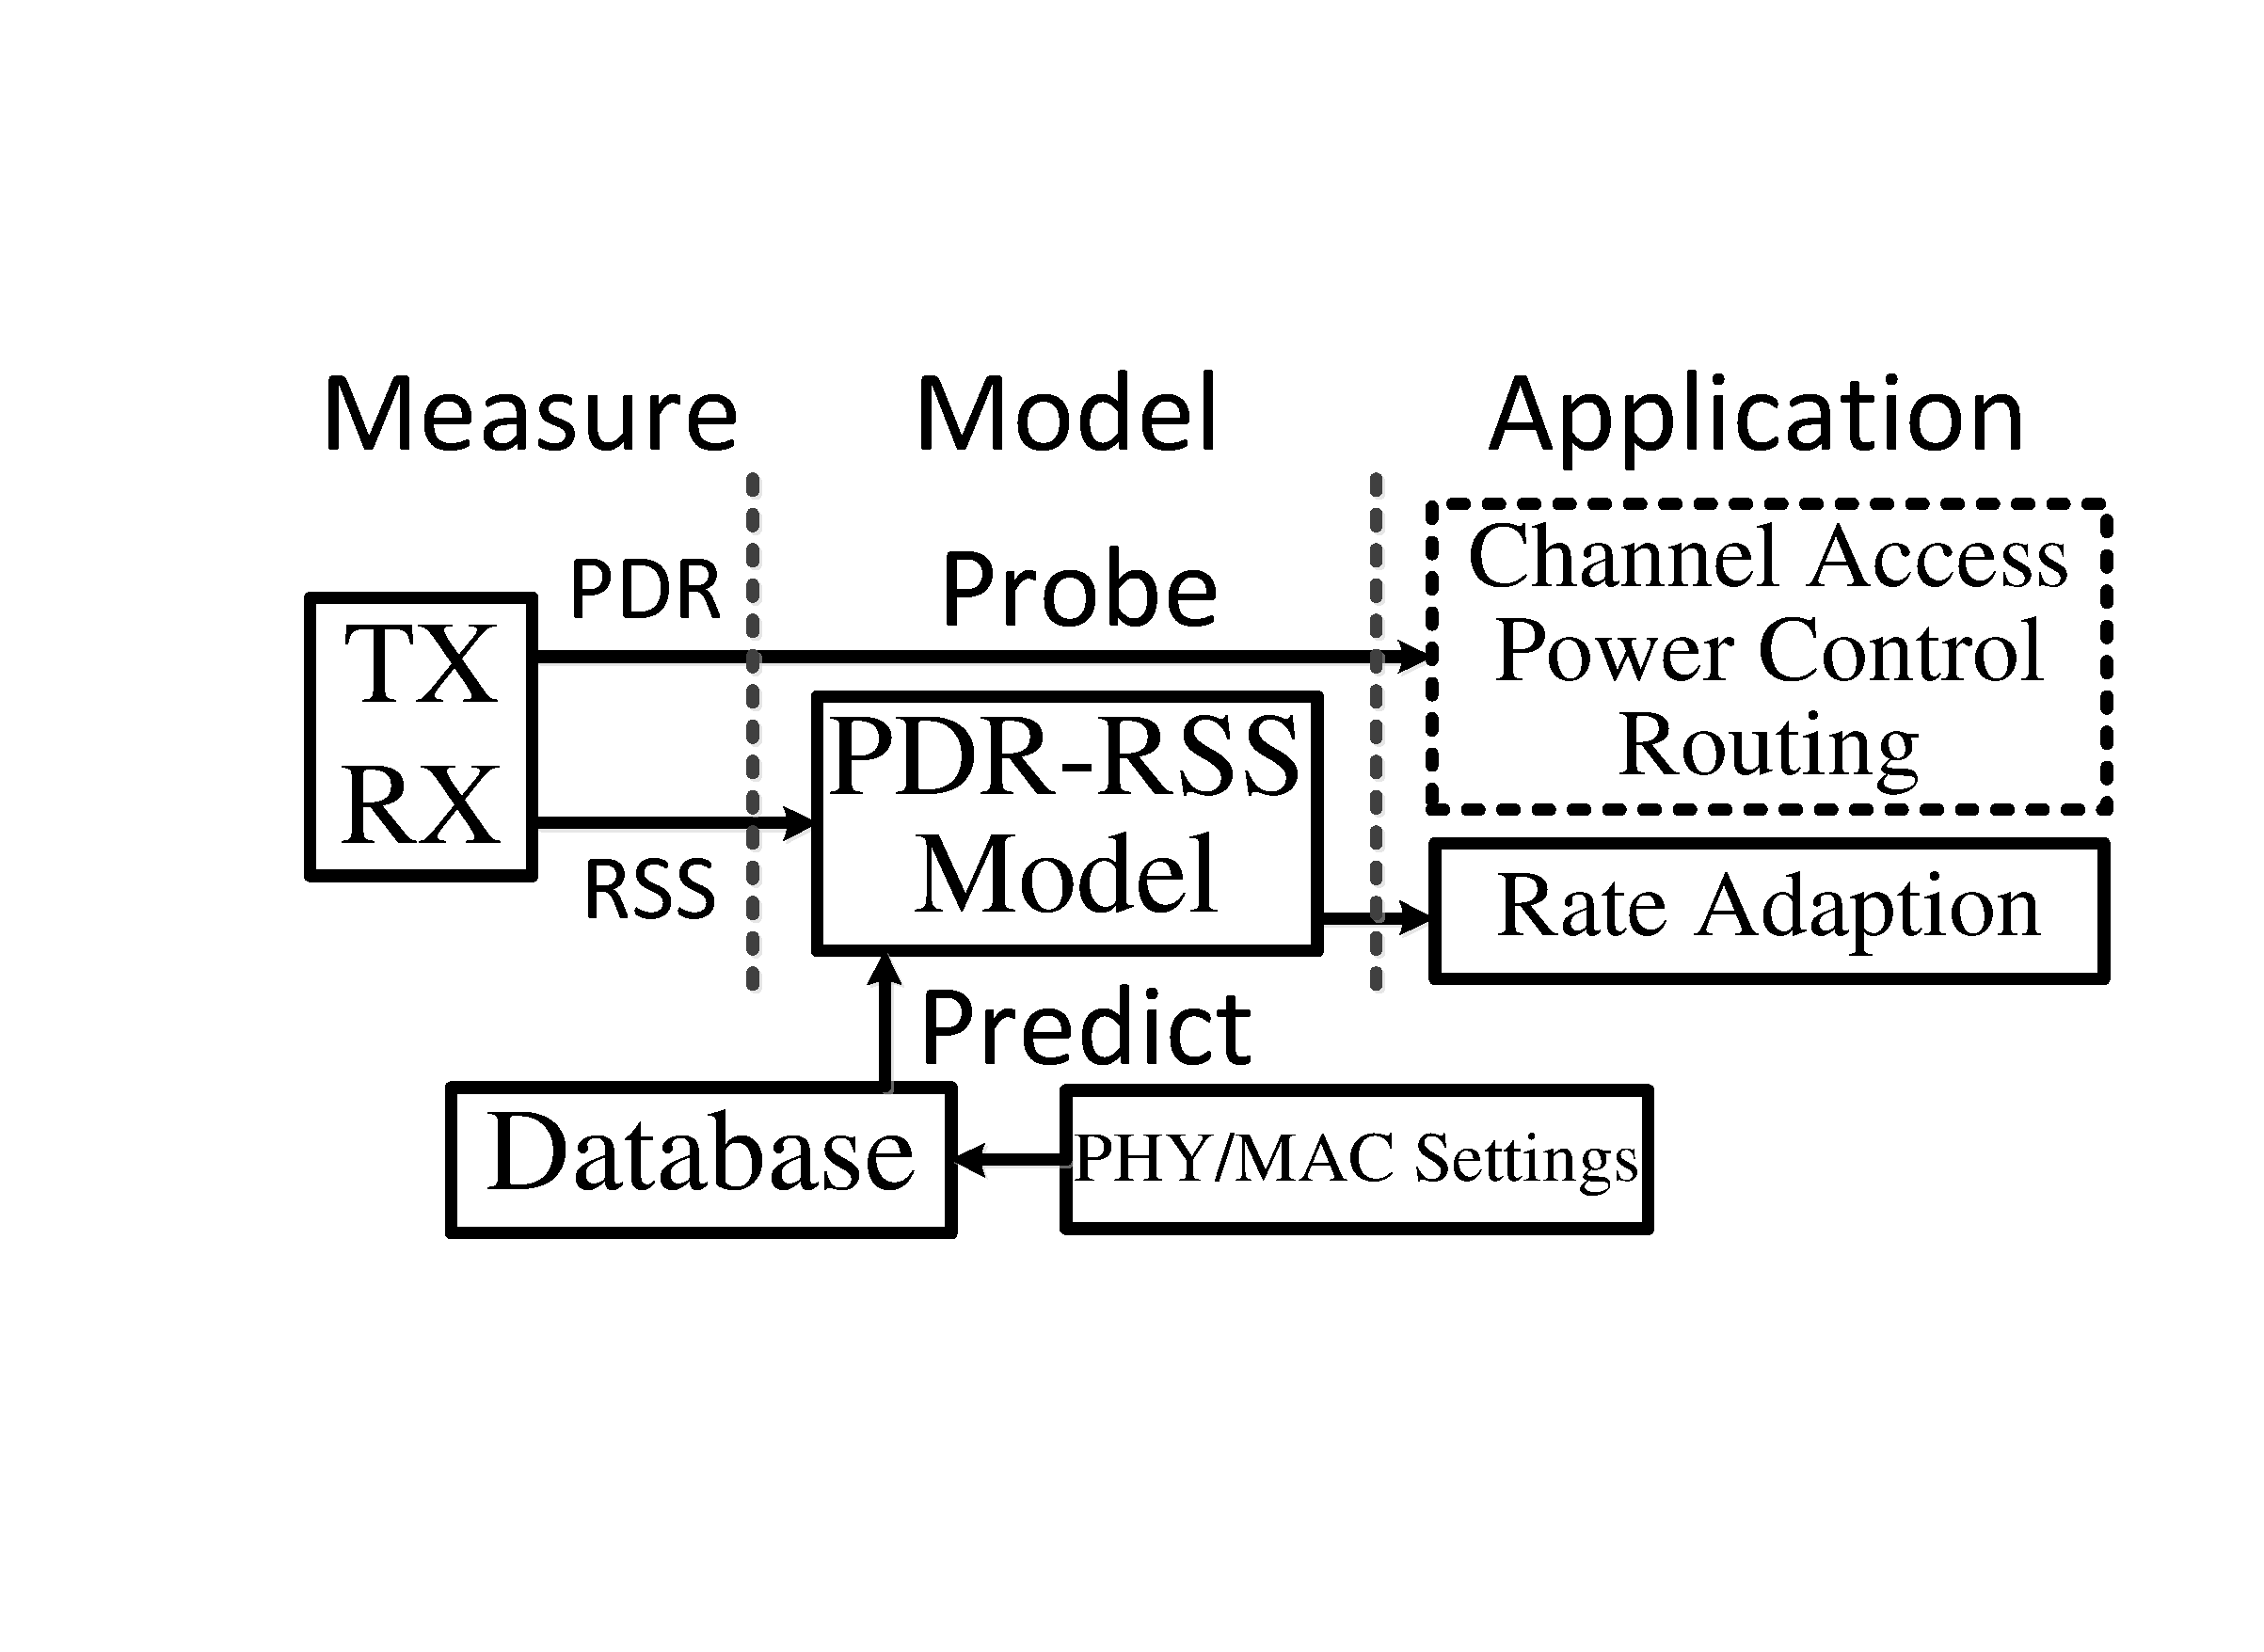
\includegraphics[width=0.6\textwidth]{chap3/modeling1.pdf}
\bicaption[fig:offlinemodel]{静态链路质量-信道状态模型}{静态链路质量-信道状态模型}{Fig}{General static PDR-RSS modeling framework}
\end{figure}

传统无线网络的上层应用,包括速率适配、功率控制及路由策略等,都不可避免地需要底层的网络状态信息,比如物理层信道状态或链路层链路质量。图 \ref{fig:offlinemodel} 所示为基于静态PDR-RSS模型的应用框架,本文中以速率控制为例进行详细介绍。从图中可以看出,基于静态PDR-RSS模型的速率控制算法主要分为两类:第一类通过探测数据包对链路层链路质量进行实时测试,直接根据当前链路质量进行速率选择;第二类利用静态PDR-RSS模型,根据当前物理层信道信息对网络状态进行预测,并作出相应配置选择。

以上的静态PDR-RSS框架无法之际应用于移动MIMO-OFDM系统中:第一,由于移动无线网络在运行过程中外界环境与网络状态复杂多变,从而降低链路质量的测试精度;第二,由于802.11n系统采用了多种物理层和链路层配置,从而增加了链路质量的测试开销;第三,MIMO-OFDM的多配置特性增加了PDR-RSS模型的复杂性\footnote{多种配置需要分别进行建模,同时MIMO-OFDM系统的PDR-RSS模型具有过渡窗口效应}。所以移动802.11n网络的移动性和多配置性降低了链路质量的测试与预测精度,进一步影响网络的整体性能。

\subsection{存在问题}
\label{sec:prob3}

本节通过大量实验数据说明以上静态框架应用于移动802.11n网络中存在的问题,从而引入移动MIMO-OFDM系统中链路质量测试与建模过程中存在的关键问题。静态PDR-RSS框架的主要特点包括:
\begin{itemize}
  \item 固定参数设定的PDR测试算法
  \item 静态PDR-RSS模型与数据库
  \item 单一测量与判决指标(PDR或RSS)输入
\end{itemize}
静态PDR-RSS框架的以上特点无法满足移动性带来的网络状态的时空变化,以及多配置带来的PDR-RSS模型的过渡窗口问题。

\begin{figure}[!htp]
\centering
    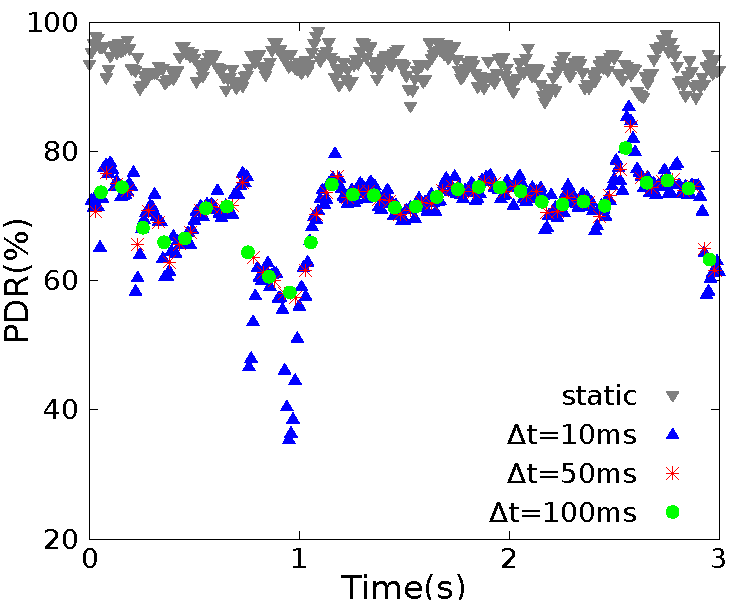
\includegraphics[width=0.8\textwidth]{chap3/pdrvary.pdf}
\bicaption[fig:pdrover]{链路质量测试误差}{链路质量测试误差}{Fig}{PDR overestimation as sudden decline}
\end{figure}

\begin{itemize}
  \item \textbf{移动网络时空特性:}
  移动网络的时空变化特性对PDR的测量精度与开销具有重要影响。无线网络中广泛应用指数加权平均算法进行链路质量测试 \cite{ath9k} \cite{minstrel} \cite{wong2008wireless},一般其参数设置为固定值,比如采样周期一般设置为50ms或100ms,而加权因子一般设置为0.25 或0.125。但是网络状态的时空变化会降低EWMA算法的测试精度,尤其当网络运行与较高数据传输速率时。图 \ref{fig:pdrover} 所示的实验结果说明了网络状态变化对PDR测试的影响,当被测PDR发生瞬时变化时,采样周期固定为50ms或100ms的EWMA算法无法获得准确的PDR信息,甚至出现20\%的测试误差。因此有必要对PDR测试算法进行改进,以提高移动网络中链路质量测试精度。现有的针对移动网络链路质量测试方法的工作主要针对RSS的测试 \cite{chen2011ram} \cite{judd2008efficient}。
  \item \textbf{MIMO-OFDM系统过渡窗口:}
  MIMO-OFDM系统的多种配置增加了链路质量测试与预测的复杂度。由于802.11n网络采用了多种物理层和链路层技术,同时网络运行时需要在多种配置间进行切换,从而增加了链路质量测试的复杂度,MIMO-OFDM系统中PDR-RSS模型的过渡窗口进一步增加了802.11n网络中PDR-RSS建模的复杂度 \cite{Halperin2010predictable}。如图 \ref{fig:transition} 所示,802.11n网络的PDR-RSS模型存在3-15dB的过渡窗口长度,对于静态建模框架约有34\%的被选配置落入过渡窗口,甚至有8\%的配置位于过渡窗口左侧\footnote{落入过渡窗口表示PDR<$P_{thrh}$=90\%,位于过渡窗口左侧表示PDR<$P_{thrl}$=10\%}。因此有必要针对MIMI-OFDM系统的多配置特性,设计有效的PDR-RSS建模方法与配置选择策略。
\end{itemize}

\begin{figure}[!htp]
\centering
    \subfigure[PDR-RSS模型]{
    \label{fig:pdr-rss}
    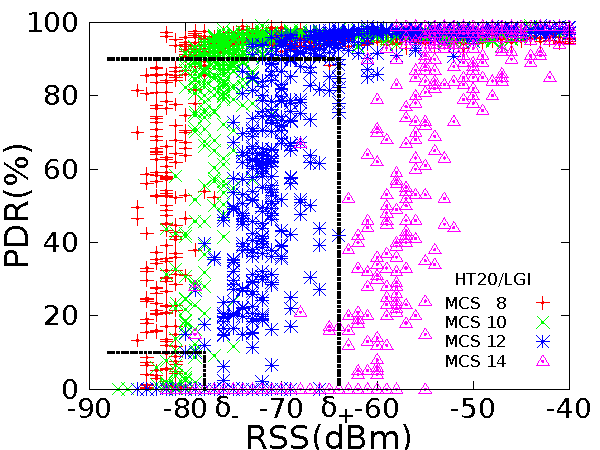
\includegraphics[width=0.46\textwidth]{chap3/pdr.pdf}}
    \hspace{1cm}
    \subfigure[过渡窗口]{
    \label{fig:MCS}
    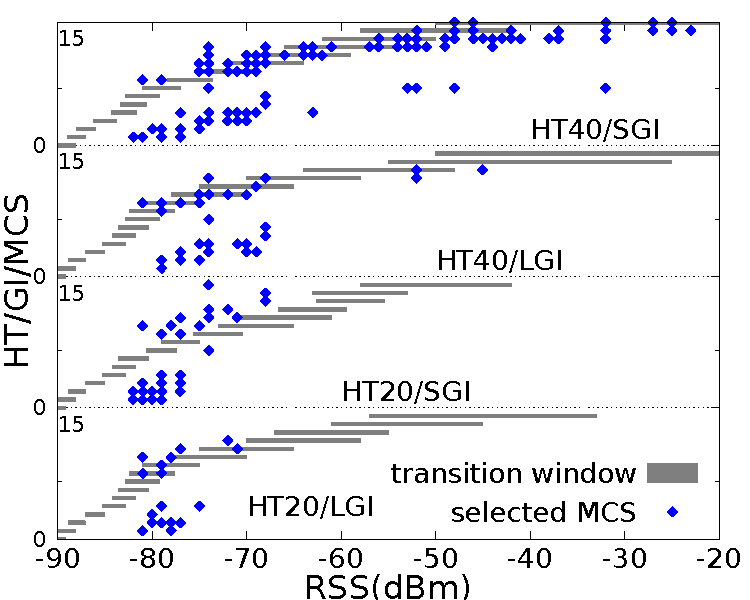
\includegraphics[width=0.44\textwidth]{chap3/MCS.pdf}}
\bicaption[fig:transition]{PDR-RSS模型过渡窗口}{PDR-RSS模型过渡窗口}{Fig}{Transition windows of PDR-RSS model as high data rates}
\end{figure}

802.11n网络的物理层和链路层配置一方面显著提升网络性能,但是同时使得链路质量测试与建模更为复杂。移动终端造成网络状态的时空变化特性,从而对链路质量测试的精度与开销提出更高要求。本文提出在线建模框架以有效解决一下问题:(1)动态链路质量测试算法;(2)在线PDR-RSS建模与实时更新机制;(3)高效准确的多配置选择策略。

\section{链路质量动态测试}
\label{sec:measure}

\subsection{信号传输模型}
\label{sec:packetmodel}

为了对不同的链路质量测试方法进行刻画,并对不同测试方法进行分析,首先引入数据包传输模型。发送数据包的接收状态可以认为是离散随机过程$X=\{x_1, x_2, ... x_i\}$,而每一个数据包的接收状态为0或1,即$x_i=\{0, 1\}$, $i(i=1,2,3...)$,其中$x_i=1$表示第$i$个数据包成功接收。第$i$个数据包成功接收的概率$\textbf{P(}x_i=1\textbf{)}=p_i$可以由标准的信噪比模型来刻画,如下式所示:
\begin{equation}
 p_i=\textbf{P(}SINR_i(t)>\delta\textbf{)}=\textbf{P(}\frac{R_i(t)}{I_i(t)+n}>\delta\textbf{)}
\label{equa:p_i}
\end{equation}
其中$SINR_i(t)$为第$i$个接收数据包在$t$时刻的信噪比,$\delta$为信噪比门限值,$R_i(t)$为接收数据包在时刻$t$的接收信号强度,$I_i(t)$ 为除传输信号外其他信号$R_j(t)$造成的接收端信号干扰,$n$为热噪声且一般为恒定值。同时$p_i$可以由实测模型表示,即
\begin{equation}
 p_i=\hat{p}(R_i(t))
\label{equa:p_i_measure}
\end{equation}
其中$\hat{p}(R_i(t))$为基于实测数据的传输成功率,表示为接收信号强度的函数。

\subsection{传统测试方法}
\label{sec:traditional}

\begin{figure}[!htp]
\centering
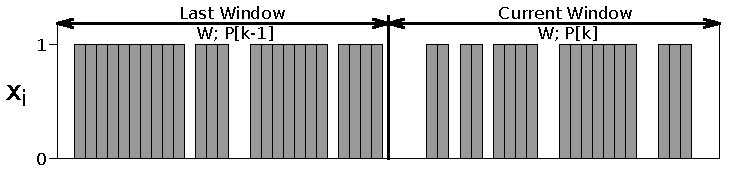
\includegraphics[width=5in]{chap3/m_weighted.pdf}
\bicaption[fig:weighted]{静态加权平均}{静态加权平均}{Fig}{EWMA with fixed $W$ and $\alpha$}
\end{figure}

对于静态无线网络中的传输成功率测试,在统计区间内的数据包的接收状态可以认为常数,且$x_i$为独立同分布的随机变量,即$P(x_i=1)=p_i=p$,此时$X$可以刻画为伯努利过程,即$X\sim B(p)$。一般采用固定窗口长度进行平均,如图 \ref{fig:weighted} 所示,第$k$次测试的传输成功率为
\begin{equation}
PDR_f[k]=\frac{1}{W}\sum_{i=kW+1}^{(k+1)W}{x_i}
\label{equa:pdr_f}
\end{equation}
其中$W$为平均窗口长度。此时的测试误差可以表示为测试传输成功率与接收成功概率的差,因此测试误差的期望与方差分别为:
\begin{equation}
 \textbf{E[}\Delta PDR_f\textbf{]}=\textbf{E[}\frac{1}{W}\sum_{i=1}^{W}{x_i}-p\textbf{]}=\frac{1}{W}\sum_{i=1}^{W}{\textbf{E[}x_i\textbf{]}}-p=0
\label{equa:Epf}
\end{equation}
\begin{equation}
 \textbf{D[}\Delta PDR_f\textbf{]}=\textbf{D[}\frac{1}{W}\sum_{i=1}^{W}{x_i}-p\textbf{]}=\frac{1}{W}\sum_{i=1}^{W}{\textbf{D[}x_i\textbf{]}}=p(1-p)
\label{equal:Dpf}
\end{equation}
其中$\overline{p}[k]$与$\overline{p'}[k]$分别为$P[k]$与$P'[k]$的估计值,可以由式(\ref{equa:Epf})获得,即
\begin{equation}
 \textbf{E[}P[\cdot]\textbf{]}=\frac{1}{N}\sum\textbf{E[}x_i\textbf{]}=\frac{1}{N}\sum{p_i}=\overline{p}[\cdot]
\label{equal:pestimation}
\end{equation}
其中$N$为窗口长度,$\overline{p}[\cdot]$为该统计区间内$p_i$的算术平均值,$p_n$当前时刻发送数据包的接收概率并作为传输成功率的真实值。从式(\ref{equal:pestimation})可以看出测试误差与$p_i$的变化情况密切相关,而$p_i$在静态无线网络与移动无线网络中呈现不同的特性。同时平均窗口长度$W$ 对于测试误差具有很大影响,例如当$p_i$在短时间尺度内出现剧烈变化时,过大的窗口长度会丢失传输成功率的细节信息。

在实际系统中一般采用指数加权平均,即EWMA算法,例如在Atheros's Linux系统的无线驱动中,包括针对802.11a/b/g网络的\texttt{Madwifi} \cite{madwifi} 以及用于802.11n网络的\texttt{ath9k} \cite{ath9k},以提高测试精度并降低测试开销。在EWMA中测试传输成功率表示为当前测试结果与历史结果的加权平均,即
\begin{equation}
 PDR_w[k]=\alpha PDR_f[k-1]+(1-\alpha)PDR_f[k]
\label{equal:pdr_w}
\end{equation}
其中$\alpha$为加权因子。此时EWMA的测试误差为:
\begin{equation}
\begin{split}
 \textbf{E[}\Delta PDR_w\textbf{]}&=\textbf{E[}\alpha PDR_f+(1-\alpha)PDR_f-p\textbf{]}\\
         &=\alpha \textbf{E[}PDR_f\textbf{]}+(1-\alpha)\textbf{E[}PDR_f\textbf{]}-p\\
         &=\alpha p + (1-\alpha) p-p\\
         &=0
\end{split}
\label{equa:Epw}
\end{equation}

\begin{equation}
\begin{split}
 \textbf{D[}\Delta PDR_w\textbf{]}&=\textbf{D[}\alpha PDR_f+(1-\alpha)PDR_f-p\textbf{]}\\
         &=\alpha^2\textbf{D[}PDR_f\textbf{]}+(1-\alpha)^2\textbf{D[}PDR_f\textbf{]}\\
         &=[\alpha^2+(1-\alpha)^2]p(1-p)
\end{split}
\label{equa:Dpw}
\end{equation}

从以上的分析可以看出,在静态无线网络传输成功率测试中,固定窗口与加权算法都可以获得无偏估计,而加权算法在不增加测试开销的前提下具有更低的均方差,由式(\ref{equa:Dpw})可以得出当$\alpha=0.5$时,理论上可以得到最小均方差$\textbf{D[}PDR_w\textbf{]}$。对于如图 \ref{fig:mobile_k} 中给定的接收成功概率$p\sim N(0.8, 0.01)$,相对于固定窗口测试方法,加权算法可以获得更准确的测试结果。如图 \ref{fig:static_e} 所示,固定窗口算法测试结果为80.23\%,而$\alpha=0.5$时的加权算法测试结果为80.06\%,可以看到两者的测试误差都很小,且固定窗口算法的均方差为0.0268,而加权算法在$\alpha=0.5$ 时的均方差为0.0034。

\begin{figure}[!htp]
\centering
\subfigure[原始平均 ($\alpha=0$)]{
    \label{fig:fixed_s}
    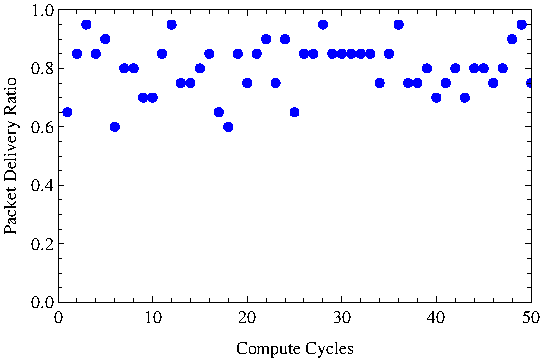
\includegraphics[width=2.5in]{chap3/fixed_n.pdf}}
    \hspace{1cm}
\subfigure[加权平均 ($\alpha=0.5$)]{
    \label{fig:weighted_s}
    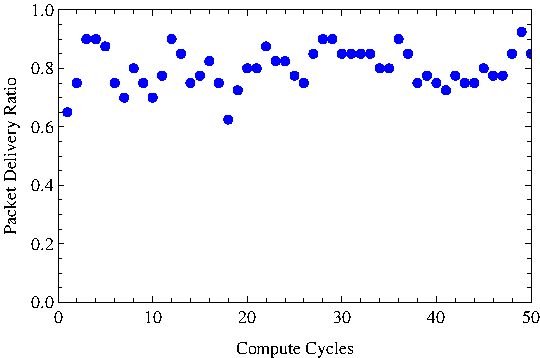
\includegraphics[width=2.5in]{chap3/weighted_n.pdf}}
\bicaption[fig:static]{静态网络测试精度}{静态网络测试精度}{Fig}{Measurement Window Length in Static Wireless Networks ($W=20, p=0.8$)}
\end{figure}

\begin{figure}[!htp]
\centering
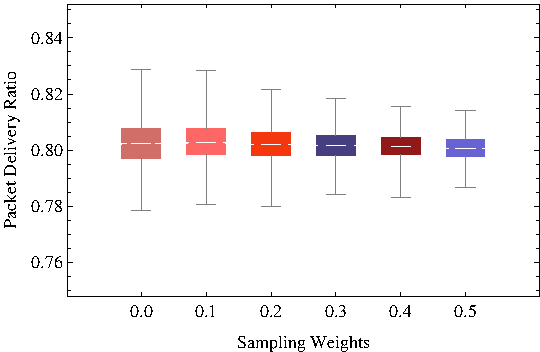
\includegraphics[width=5in]{chap3/static.pdf}
\bicaption[fig:static_e]{测试精度 ($\alpha=0\sim0.5$)}{测试精度 ($\alpha=0\sim0.5$)}{Fig}{Measurement Accuracy for Weighted Averaging}
\end{figure}

但是在实际测试中,加权因子$\alpha$一般在0.1到0.4之间取值,主要原因是$p_i$并不保持不变,而在移动无线网络中这种情况更为明显,因此当固定加权算法应用在移动无线网络测试中时,无法保证传输成功率的测试精度,从而影响网络性能,主要有以下原因:

\begin{itemize}
  \item 平均窗口长度以时间计量并为固定值,一般设置为50ms或100ms,难以对802.11n网络的多种配置进行有效测试;
  \item 合适的加权因子难以选择,理论上$\alpha$应设置在0.1到0.3之间 \cite{EWMAChart},在实际中一般选择固定值0.125 \cite{ath9k}或0.25 \cite{minstrel}。
\end{itemize}

以上两点造成加权算法无法对测试精度与测试开销进行有效地控制,因此有必要针对移动802.11n网络的时空多变及多配置特性,提出有效地传输成功率测试算法,以适应链路质量的变化并有效调整测试精度与开销。

\subsection{动态滑动平均}
\label{sec:sliding}

对于移动无线网络传输成功率的测试而言,需要考虑测试精度与开销的权衡与折中问题。一方面其测量周期需要尽量短,以适应移动终端接收信号强度的突变并提高测试精度;另一方面在网络状态稳定或传输速率较低时,需要降低采样频率以减小对网络可用资源的影响并降低测试开销。

由于无线网络无线传播环境的复杂性,尤其对于移动网络与移动终端而言,造成接收信号强度和干扰的在传输成功率测量过程中的时空变化特性,使得数据包接收成功概率$p_i$在短时间尺度内变化;同时由于802.11n网络采用了MIMO-OFDM技术,造成其物理层与链路层的多配置特性,从而造成链路质量测试复杂性的升高及有效性的降低。因此有必要对原有加权算法进行改进,以适应移动网络的时空特性,并适应MIMO-OFDM系统的多配置特性。

\begin{figure}[!htp]
\centering
    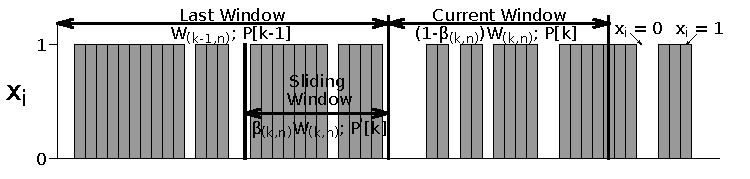
\includegraphics[width=5in]{chap3/m_sliding.pdf}
\bicaption[fig:sliding]{动态滑动平均}{动态滑动平均}{Fig}{DSWA with dynamic $W$ and $\beta$}
\end{figure}

针对以上问题,本文提出基于动态滑动窗口平均的传输成功率测试算法,如图 \ref{fig:sliding} 所示,当前测试窗口与上一测试窗口间存在重叠区域,即滑动窗口。在DSWA中PDR的测量值为
\begin{equation}
 \hat{P_s}[k]=\beta P'[k]+(1-\beta)P[k]
 \label{equa:P_s}
\end{equation}
其中$T$和$W$分别为滑动窗口和当前平均窗口长度,$\beta=\frac{T}{W}$滑动窗口与当前窗口比率,定义为为滑动因子,$P'[k]$和$P[k]$分别代表滑动窗口和当前窗口的PDR测量值。DSWA中$W$和$\beta$的设置对于传输成功率的测试精度和误差有着重要影响,第$k$次测量周期的窗口长度$\overline{W}_{(k,n)}$ 与滑动因子$\overline{\beta}_{(k,n)}$分别定义为
\begin{equation}
  \overline{W}_{(k,n)} = \frac{\sum_{i=1}^n{\omega_i \gamma_i} \eta_{i}}{\sum_{i=1}^n{\omega_i}}
\label{equa:W_s}
\end{equation}
\begin{equation}
  \overline{\beta}_{(k,n)} = 1 + \frac{\sum_{i=1}^n{\omega_i \gamma_i}}{\sum_{i=1}^n{\omega_i}}
\label{equa:beta}
\end{equation}
其中$\omega_i$为加权因子,本文中定义为
\begin{equation}
  \omega_i = \frac{1}{2^{\lfloor\frac{n-i}{2}\rfloor}},~1\leq i \leq n,
\label{equa:omega_i}
\end{equation}
$\gamma_i$为中间变量,代表当前PDR的变化情况,表示为
\begin{equation}
  \gamma_i = 1 + P[k-n+i] - P[k-n+i-1],~~ 1 \leq i \leq n,
\label{equa:gamma_i}
\end{equation}
其中$\eta$为之前$n$个测量周期的窗口长度,即$\eta_i=W_{(k-n+i,n)}$。在实际应用中,加权长度设置为$n=8$,加权因子设置为$\omega_i=\{1/8,1/8,1/4,1/4,1/2,1/2,1,1\}$,以充分利用历史数据并尽量提高当前信息的比例,从而可以根据网络当前状态兼顾测试的灵敏性与稳定性,同时1/2 幂次方的设置也使得程序的运算与执行更为高效。与EWMA不同的是,DSWA并非通过时间驱动,因此其测试周期与传输速率无关,同时DSWA通过滑动窗口强调当前网络状态,由于$\omega_i$和$\gamma_i$的设置与PDR的相对变化有关,DSWA可以通过$W$和$\beta$的调整与当前网络状态相匹配。

通过图 \ref{fig:sliding} 及式(\ref{equa:P_s})可以得到
\begin{equation}
  \textbf{E[}P[\cdot]\textbf{]}=\frac{1}{N}\sum\textbf{E[}x_i\textbf{]}=\frac{1}{N}\sum{p_i}=\overline{p}[\cdot]
\label{equa:epinter}
\end{equation}
\begin{equation}
  \textbf{D[}P[\cdot]\textbf{]}=\frac{1}{N^2}\sum\textbf{D[}x_i\textbf{]}=\frac{1}{N^2}\sum{p_i(1-p_i)}=\frac{1}{N}\overline{q}[\cdot]
\label{equa:dpinter}
\end{equation}
其中$N$为采样数目,$\overline{p}[\cdot]$和$\overline{q}[\cdot]$分别为$p_i$和$p_i(1-p_i)$的算数平均值,从而DSWA的测量误差可以表示为
%\begin{equation}
%\begin{split}
% \textbf{E[}\Delta PDR_s[k+1]\textbf{]}&=\textbf{E[}\frac{1}{W}\textstyle\sum_{k(W-T)}^{(k+1)W-kT}{x_i}-p_{n}\textbf{]}\\
%              &=\frac{1}{W}\textstyle\sum_{k(W-T)}^{(k+1)W-kT}{\textbf{E[}x_i\textbf{]}-p_{n}}\\
%              &=\frac{1}{W}\textstyle\sum_{k(W-T)}^{(k+1)W-kT}{p_i}-p_{n}\\
%              &=\overline{p}_{k+1}-p_{n}
%\end{split}
%\label{Eps}
%\end{equation}
%
%\begin{equation}
%\begin{split}
% \textbf{D[}\Delta PDR_s[k+1]\textbf{]}&=\textbf{D[}\frac{1}{W}\textstyle\sum_{k(W-T)}^{(k+1)W-kT}{x_i}-p_{n}\textbf{]}\\
%              &=\frac{1}{W^2}\textstyle\sum_{k(W-T)}^{(k+1)W-kT}{\textbf{D[}x_i\textbf{]}}\\
%              &=\frac{1}{W^2}\textstyle\sum_{k(W-T)}^{(k+1)W-kT}{p_i(1-p_i)}\\
%              &=\frac{1}{W}\overline{q}_{k+1}
%\end{split}
%\label{Dps}
%\end{equation}
\begin{equation}
\begin{split}
 \textbf{E[}\Delta PDR_s[k+1]\textbf{]}&=\textbf{E[}\beta P'[k]+(1-\beta)P[k+1]-p_{n}\textbf{]}\\
                                       &=\beta\textbf{E[}P'[k]\textbf{]}+(1-\beta)\textbf{E[}P[k+1]\textbf{]}-p_{n}\\
                                       &=\beta\overline{p'}[k]+(1-\beta)\overline{p}[k+1]-p_{n}
\end{split}
\label{equa:Eps}
\end{equation}

\begin{equation}
\begin{split}
 \textbf{D[}\Delta PDR_s[k+1]\textbf{]}&=\textbf{D[}\beta P'[k]+(1-\beta)P[k+1]-p_{n}\textbf{]}\\
                                       &=\beta^2\textbf{D[}P'[k]\textbf{]}+(1-\beta)^2\textbf{D[}P[k+1]\textbf{]}\\
                                       &=\frac{\beta\overline{q'}[k]+(1-\beta)\overline{q}[k+1]}{W}
\end{split}
\label{equa:Dps}
\end{equation}
其中$\overline{p}[k+1]$和$\overline{q}[k+1]$分别为$p_i$和$p_i(1-p_i)$在第$(k+1)$测量周期的平均值,$\overline{p'}[k]$和$\overline{q'}[k]$为滑动窗口部分估计值,$p_n=p_{(k+1)W-kT}$为第$((k+1)W-kT)$个数据包的接收成功概率。

\begin{figure}[!htp]
\centering
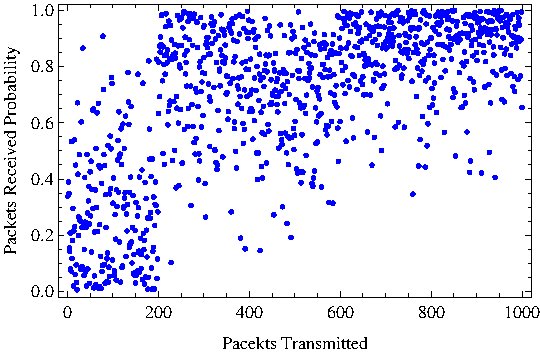
\includegraphics[width=5in]{chap3/mobile.pdf}
\bicaption[fig:mobile_k]{数据包接收成功概率}{数据包接收成功概率}{Fig}{Packets Received Probability}
\end{figure}

从式(\ref{equa:Eps})和式(\ref{equa:Dps})可以看出,DSWA的测量误差同样与$p_i$的变化情况有关,总体上相对于EWMA在移动网络条件下具有更高的精度与测试开销。如图 \ref{fig:mobile} 所示,当$p_i$同样设置为图 \ref{fig:mobile_k} 中情形时,DSWA以同样的窗口长度能够实现更频繁的采样,同时具有更高的测量精度,相对于EWMMA的0.19到0.32的测量误差,DSWA在$\beta=0.3$时能够将测量误差降低为0.001。

\begin{figure}[!htp]
\centering
\subfigure[Weighted Window Length $(\alpha=0.4)$]{
    \label{fig:weighted_m}
    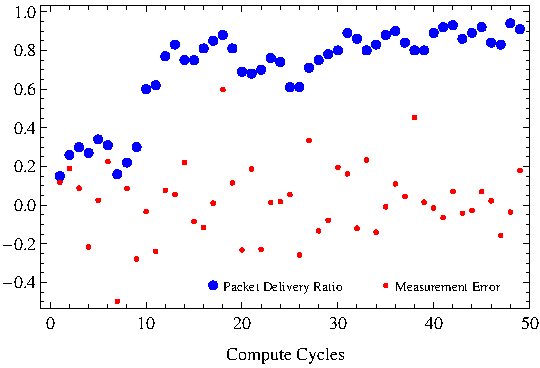
\includegraphics[width=2.5in]{chap3/weighted_m.pdf}}
    \hspace{1cm}
\subfigure[Sliding Window Length $(\beta=0.3)$]{
    \label{fig:sliding_m }
    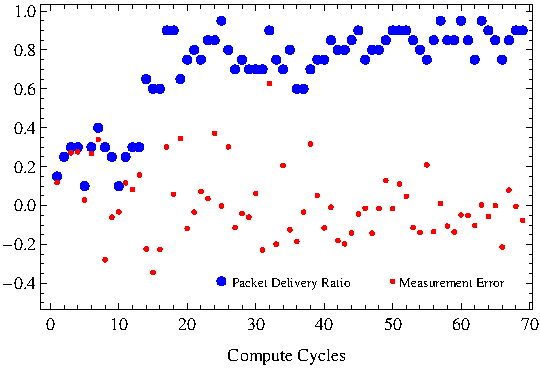
\includegraphics[width=2.5in]{chap3/sliding_m.pdf}}
\bicaption[fig:mobile]{移动网络测试精度}{移动网络测试精度}{Fig}{Measurement Window Length in Mobile Wireless Networks ($W=20$)}
\end{figure}

\begin{table}[!htp]
\renewcommand{\arraystretch}{1}
\bicaption[tab:footnote]{加权算法测试误差}{加权算法测试误差}{Table}{Measurement Error of Weighted Window Length}
  \centering
\begin{threeparttable}[b]
\label{error}
\begin{tabular}{c|ccccc}
\hline
$\pmb{\alpha}$ & 0.1   & 0.2   & 0.3   & 0.4   & 0.5 \\
\hline
$\textbf{E[}\Delta PDF_w\textbf{]}$  & 0.026 & 0.032 & 0.019 & 0.020 & 0.029 \\
$\textbf{D[}\Delta PDF_w\textbf{]}$  & 0.035 & 0.032 & 0.032 & 0.036 & 0.040 \\
\hline
\end{tabular}
\end{threeparttable}
\end{table}

\begin{table}[!htp]
\renewcommand{\arraystretch}{1}
\bicaption[tab:footnote]{滑动算法测试误差}{滑动算法测试误差}{Table}{Measurement Error of Sliding Window Length}
\centering
\begin{threeparttable}[b]
\label{error}
\begin{tabular}{c|ccccccccc}
\hline
$\pmb{\beta}$ & 0.1   & 0.2   & 0.3   & 0.4   & 0.5   & 0.6   & 0.7   & 0.8   & 0.9 \\
\hline
$\textbf{E[}\Delta PDF_s\textbf{]}$ & 0.040 & 0.003 & 0.001 & 0.010 & 0.015 & 0.013 & 0.008 & 0.021 & 0.007 \\
$\textbf{D[}\Delta PDF_s\textbf{]}$ & 0.036 & 0.037 & 0.038 & 0.029 & 0.039 & 0.038 & 0.029 & 0.038 & 0.036 \\
\hline
\end{tabular}
\end{threeparttable}
\end{table}

\begin{figure}[!htp]
\centering
\subfigure[a=1,b=3]{
    \label{fig:error1}
    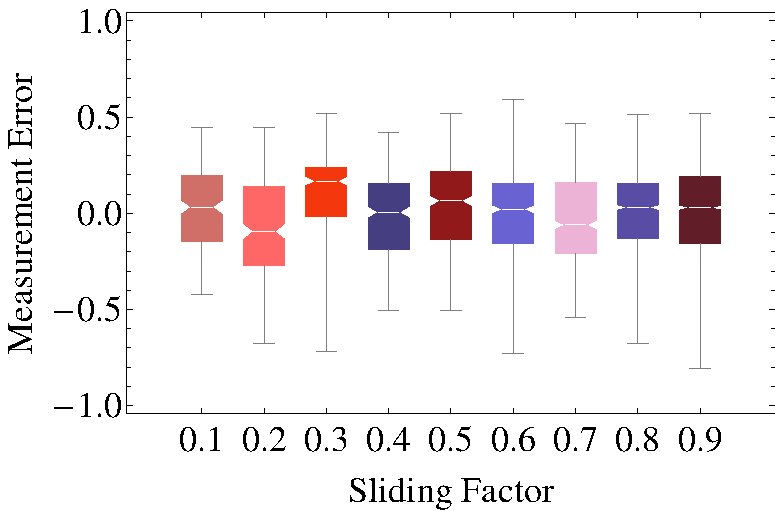
\includegraphics[width=2.5in]{chap3/error1.pdf}}
    \hspace{1cm}
\subfigure[a=3,b=1]{
    \label{fig:error2}
    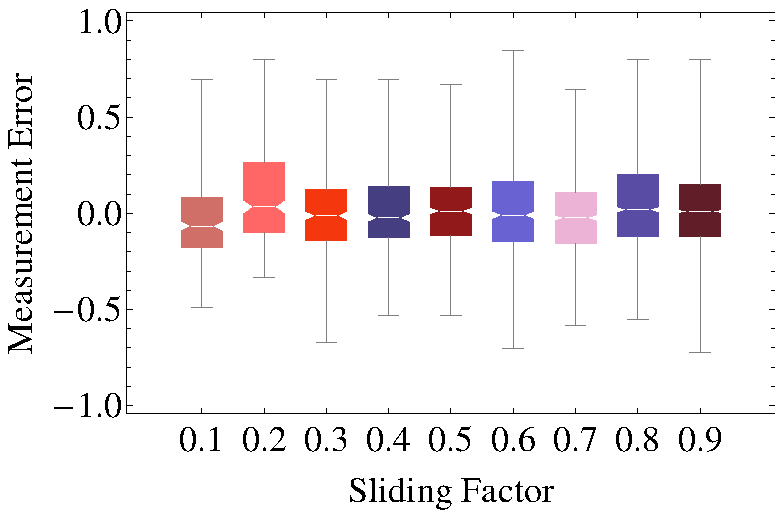
\includegraphics[width=2.5in]{chap3/error2.pdf}}
\hspace{1in}
\centering
\subfigure[a=5,b=2]{
    \label{fig:error3}
    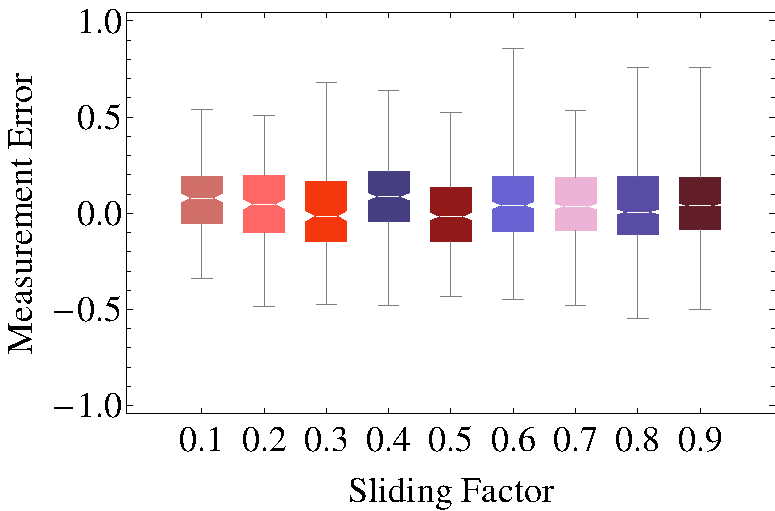
\includegraphics[width=2.5in]{chap3/error3.pdf}}
    \hspace{1cm}
\subfigure[a=5,b=1]{
    \label{fig:error4}
    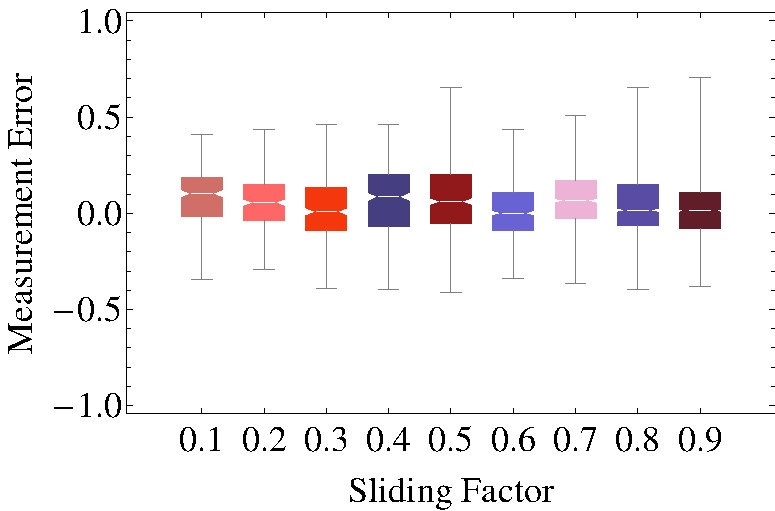
\includegraphics[width=2.5in]{chap3/error4.pdf}}
\bicaption[fig:mobile_e]{动态滑动平均测试精度}{动态滑动平均测试精度}{Fig}{Measurement Errors of Sliding Window Length Method}
\end{figure}
%
%\begin{figure}[!t]
%\centering
%  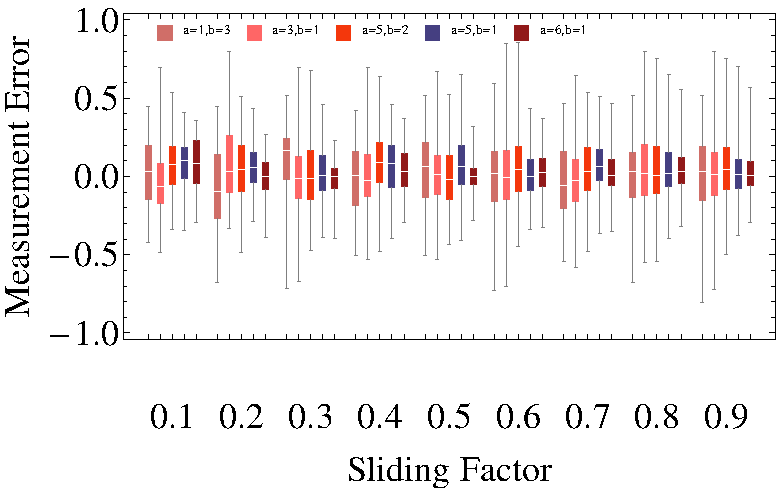
\includegraphics[width=0.5\textwidth]{error.pdf}
%\caption{Measurement Errors of Sliding Window Length Method}
%\label{mobile_e}
%\end{figure}

\section{链路质量在线建模}
\label{sec:modeling}

除了进行准确的PDR测量之外,还需要对链路层指标与物理层指标进行建模,即基于实测数据的PDR-RSS模型,并进行在线更新以提供准确的网络状态信息,从而为频谱分配及速率适配提供可靠输入。本文提出在线PDR-RSS建模框架,通过同时利用物理层及链路层信息,提高移动MIMO-OFDM网络信息的可靠传输与的速率的有效配置。在线PDR-RSS建模框架如图 \ref{fig:onlinemodel} 所示,该框架主要由三部分构成:
\begin{itemize}
  \item \textbf{PDR-RSS数据库:}PDR与RSS在不同MIMO-OFDM配置下的原始数据
  \item \textbf{PDR-RSS模型:}不同MIMO-OFDM配置下PDR-RSS模型过渡窗口上限
  \item \textbf{HT-GI-MCS索引:}MIMO-OFDM配置选择序列
\end{itemize}

\begin{figure}[!htp]
\centering
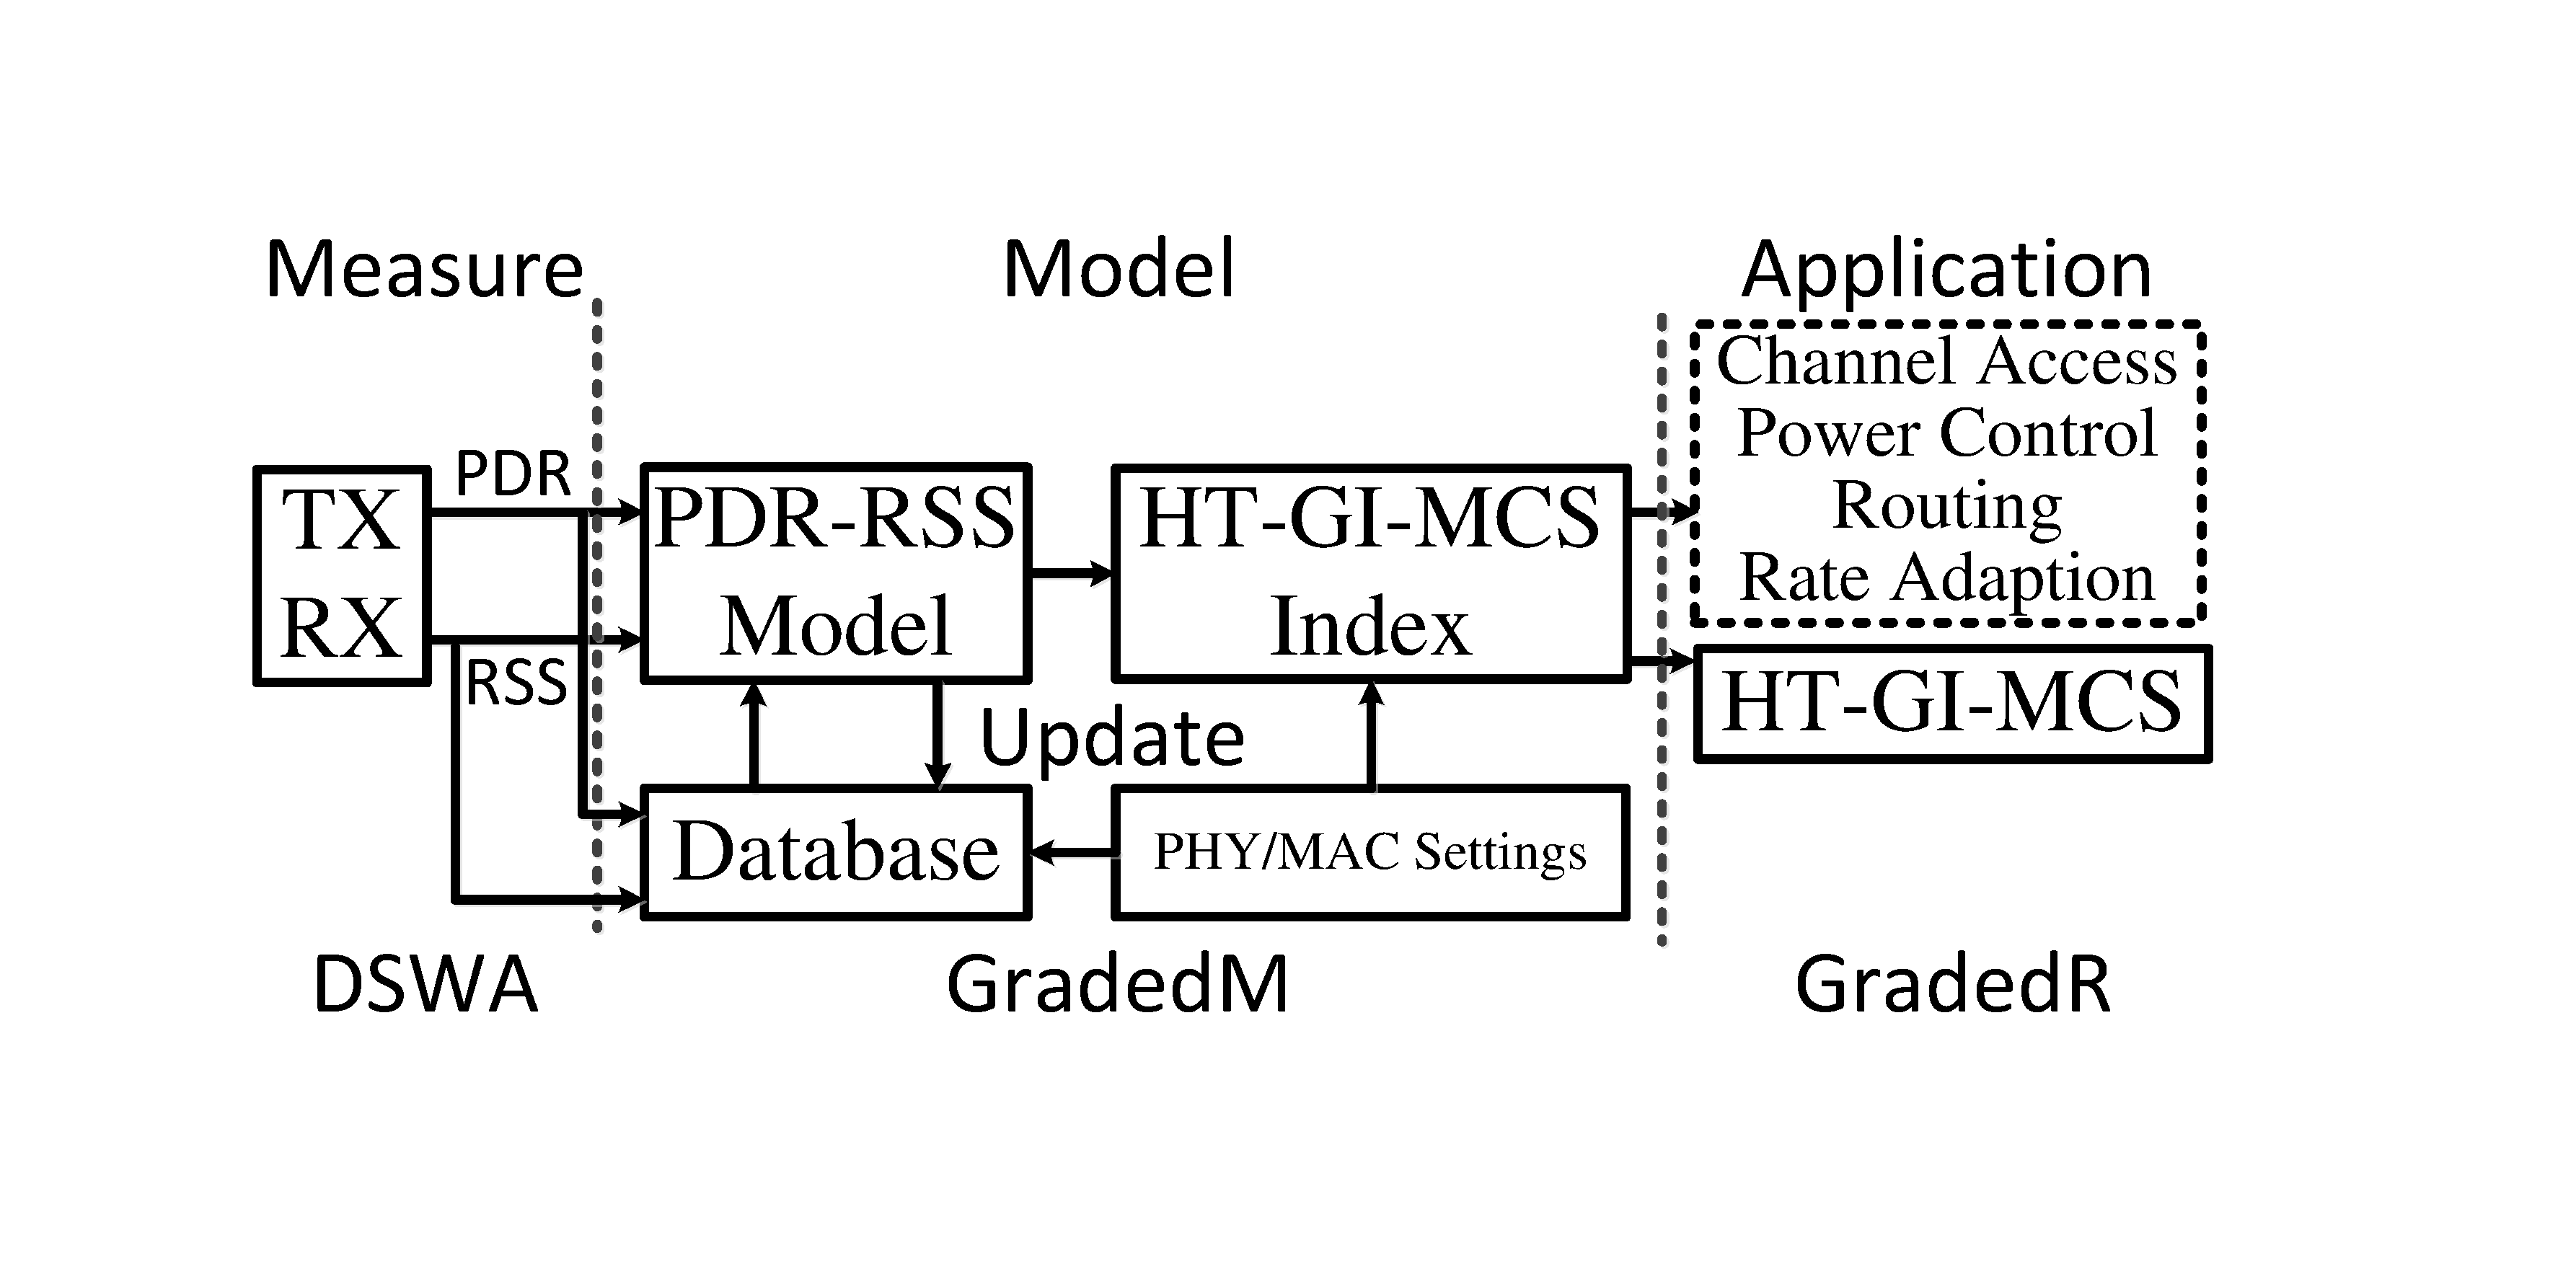
\includegraphics[width=0.8\textwidth]{chap3/modeling.pdf}
\bicaption[fig:onlinemodel]{动态PDR-RSS模型框架}{动态PDR-RSS模型框架}{Fig}{Dynamic PDR-RSS modeling framework}
\end{figure}

该框架主要由以下三步进行初始化与在线更新:
\begin{enumerate}
  \item 通过离线实验采集不同MIMO-OFDM配置下PDR及RSS的原始数据,建立PDR-RSS初始模型;
  \item 通过在线实测PDR及RSS数据对不同MIMO-OFDM配置下的PDR-RSS模型进行在线更新;
  \item 通过当前PDR及RSS相对与不同MIMO-OFDM配置下PDR-RSS模型过渡窗口上限的差值,形成MIMO-OFDM配置选择序列。
\end{enumerate}

通过以上的在线PDR-RSS建模过程,该建模框架相对于传统的静态PDR-RSS模型框架(图 \ref{fig:offlinemodel})具有明显的优点。第一,在线PDR-RSS 建模框架中数据库与PDR-RSS模型同时具有两个输入变量,而不是单独利用PDR或RSS;第二,在线框架中PDR-RSS模型和数据库同时进行在线更新,而不是只对PDR进行更新,或利用静态PDR-RSS模型而只对RSS进行更新;第三,在线框架根据当前PDR和RSS信息与模型,实时更新能够实现可靠通信的MIMO-OFDM 配置序列,并对其按照可获得性能进行排序,而不是随机探测某一配置。因此在线PDR-RSS建模框架针对静态PDR-RSS框架在信道状态和链路质量信息方面,提供了系统化的解决方案,在保证移动MIMO-OFDM网络可靠通信的前提下\footnote{在系统运行过程中保证$PDR>P_{thrh}=90\%$且$RSS>\delta_+=GradedT(HT, GI, MCS)$},提供最优的MIMO-OFDM配置选择序列。


\subsection{模型初始化}
\label{sec:initial}

802.11n标准采用多种物理层及链路层技术,实现更高的吞吐量和更广的覆盖范围。在物理层,802.11n网络利用MIMO技术实现空间复用与分集,同时利用OFDM调制方式以降低信号干扰并提升频谱利用效率,802.11n网络利用信道绑定技术可以将相邻两个20MHz的信道作为一个40MHz信道使用,从而有效提升网络吞吐量;在链路层,802.11n网络使用短保护间隔(Short Guard Interval, SGI)及帧聚合技术,以降低通信开销并提高传输效率。802.11n 网络通过以上的物理层与链路层技术,一方面能够有效提升网络性能,另一方面提高了信道状态估计和链路质量测试的复杂度,对于不同的MIMO-OFDM 配置,PDR-RSS模型具有不同特点。

为了实现802.11n网络的在线PDR-RSS建模框架,本文首先通过大量实验数据对PDR-RSS模型进行刻画,以及该模型与物理层和链路层配置的关系,主要包括信道带宽HT、调制与编码策略MCS和保护间隔长度GI。其中信道带宽分为HT=\{HT20, HT40\},保护间隔长度类型分为GI=\{LGI, SGI\},MCS与MIMO配置有关,对于3$\times$3的MIMO系统而言,MCS=\{0, 1, 2, ..., 23\}。除了网络配置之外,还需要对网络的不同位置与路线进行刻画,对802.11n 网络的PDR-RSS 模型的刻画至少需要500次重复实验,以完整包括网络的不同配置与网络状态,以下为通过这些实验数据对802.11n网络的PDR-RSS模型的总结。

\begin{figure}[!htp]
\centering
    \includegraphics[width=4in]{chap3/pdr_ch_lgi.pdf}
\bicaption[fig:pdr_lgi]{链路质量模型,HT=HT20/HT40,MCS=8-14,GI=LGI}{链路质量模型,HT=HT20/HT40,MCS=8-14,GI=LGI}{Fig}{PDR-RSS model of HT=HT20/HT40, MCS=8-14, GI=LGI}
\end{figure}

\begin{figure}[!htp]
\centering
    \includegraphics[width=4in]{chap3/pdr_ch_sgi.pdf}
\bicaption[fig:pdr_sgi]{链路质量模型,HT=HT20/HT40,MCS=8-14,GI=SGI}{链路质量模型,HT=HT20/HT40,MCS=8-14,GI=SGI}{Fig}{PDR-RSS model of HT=HT20/HT40, MCS=8-14, GI=SGI}
\end{figure}

\begin{enumerate}
  \item \textbf{信道带宽:}
  802.11n网络中定义了HT20与HT40两种信道带宽,其中HT40信道能够实现单位信号流高达150Mbps的传输速率,当链路质量能够得到有效保证时,可以获得20MHz 信道传输速率的两倍以上。但是另一方面HT40信道更容易受到信号干扰的影响,从图 \ref{fig:pdr_lgi} 可以看出,在不同的调制与编码策略及保护间隔情形下,HT40 信道的接收灵敏度明显高于HT20信道。同时可以看出HT40与HT20信道的过渡窗口长度基本相同,当MCS从8增加到14,HT20/HT40信道的过渡窗口长度从3dB变化为10dB。另一方面在适中的数据传输速率范围内,HT40信道能够在相同的传输速率基础上提供更广的覆盖范围。
  \item \textbf{调制编码:}
  不同的调制与编码策略对于802.11n网络的PDR-RSS模型具有很大影响,图 \ref{fig:pdr_lgi} 与图 \ref{fig:pdr_sgi} 刻画了在HT=HT20/HT40和GI=LGI/SGI 下PDR-RSS模型与MCS的关系。第一,接收灵敏度随着MCS的上升而增大,当MCS从8增加到14时,HT20/SGI与HT40/SGI的接收灵敏度分别在(-80dBm, -50dBm)和(-80dBm, -40dBm)范围内递增;第二,过渡窗口长度$\rho$同样随着MCS的上升而增大,尤其当传输速率高于115Mbps时,从图 \ref{fig:pdr_sgi} 中可以看出,当MCS=12时$\rho$甚至达到15dB,而过长的过渡窗口长度会严重降低网络的有效吞吐量。
  \item \textbf{保护间隔:}
  802.11n网络采用短保护间隔以进一步提升网络性能,理论上GI=SGI可以获得11\%的传输速率的提升 \cite{perahia2008next}。当传输速率较低时,SGI与LGI 的传输成功率和吞吐量没有很大分别,如图 \ref{fig:pdr_lgi} 和图 \ref{fig:pdr_sgi} 所示。但是当传输速率较高时,SGI可以明显提高网络性能,尤其对于HT40信道而言,如图 \ref{fig:pdr_sgi_high} 所示,对于HT=HT40且MCS=15时,LGI的PDR总是低于40\%,而对于HT20与HT40信道,SGI的PDR分别可以得到10\%-40\%和20\%-60\%提升。
\end{enumerate}

\begin{figure}[!htp]
\centering
    \includegraphics[width=4in]{chap3/pdr_sgi.pdf}
\bicaption[fig:pdr_sgi_high]{链路质量模型,HT=HT20/HT40,MCS=15,GI=LGI/SGI}{链路质量模型,HT=HT20/HT40,MCS=15,GI=LGI/SGI}{Fig}{PDR-RSS model of HT=HT20/HT40, MCS=15, GI=LGI/SGI}
\end{figure}

通过以上的PDR-RSS模型初始化与性质刻画,可以得到PDR-RSS的初始模型,即在不同MIMO-OFDM配置下PDR-RSS过渡窗口参数。在系统实现时定义为结构体GradedT,该结构体的初始参数可以通过复杂度为$\textit{O}(N \cdot w \cdot g \cdot r)$的实验得到,其中$N$为测试通信节点数目,$w$为某特定中心频率下的信道带宽类型, $g$为保护间隔类型,$r$为调制与编码策略数目。对于具有3$\times$3MIMO配置的802.11n系统,$w=4$代表在中心频率2.4GHz 及5GHz下分别具有HT20与HT40两种信道类型,$g=2$表示LGI和SGI两种保护间隔类型,$r=24$对应于0-23的调制与编码索引。

\begin{figure}[!htp]
\centering
    \includegraphics[width=0.8\textwidth]{chap3/graded.pdf}
\bicaption[fig:modelbegin]{PDR-RSS初始模型}{PDR-RSS初始模型}{Fig}{Initial PDR-RSS model}
\end{figure}

该PDR-RSS初始模型在系统运行时进行在线更新,2$\times$2MIMO系统的GradedT如图 \ref{fig:modelbegin} 所示,GradedT将HT/GI/MCS选择序列划分为三个区域,如果某一配置刚好位于灰色分界线的右边,则意味着该配置在当前网络状态下可以保证信号的可靠传输\footnote{即在此配置下当前RSS可以保证PDR>$P_{thrh}$=90\%},因此在当前RSS条件下所有位于灰色分界线右边的配置中,可以选择最优的配置以提高网络吞吐量。

\subsection{模型在线更新}
\label{sec:update}

在线PDR-RSS建模主要实现PDR-RSS模型与数据库的实时更新,并根据当前网络状态生成HT/GI/MCS配置选择序列,本文将这一过程简称为GradedM。首先,当RSS 或PDR其中任何某一指标低于设置的门限值时,GradedM便对PDR-RSS模型进行更新。显然,MIMO-OFDM网络某一配置在当前状态下可以获得的可靠性,可以由每一配置下PDR-RSS模型过渡窗口上限$\delta_+$ 与当前接收信号强度RSS 的距离表示,即RSS-GradedT。据此可以根据当前RSS与GradedT 进行MIMO-OFDM 配置排序,从而生成HT/GI/MCS 选择序列。以上过程的伪代码如算法 \ref{alg:graded} 所示。

\begin{algorithm}[!htp]
\floatname{algorithm}{算法}
\renewcommand{\algorithmicrequire}{\textbf{输入:}}
\renewcommand{\algorithmicensure}{\textbf{输出:}}
\caption{GradedM:PDR-RSS在线建模与实时更新}
\label{alg:graded}
\begin{algorithmic}[1]
\Require pdr-now, rss-now
\Ensure  ht-gi-mcs-index
\State{\label{graded-table}struct GradedT \{ \\ ~~~~~~~~~graded-delta[r][2]; // r=8/16/24 对应于天线数量1/2/3\\ \} graded-table[w][g]; // w=g=2 对应于信道HT20/HT40与保护间隔LGI/SGI\label{graded-table2}}
\State{// 1. PDR-RSS模型实时更新}
\If{graded-delta-changed} \label{delta-changed}
\State{graded-table $\gets$ update-delta(pdr-now,rss-now);}
\EndIf \label{delta-updated}
\State{// 2. HT/GI选择序列排序}
\State{mcs-index $\gets$ sort(graded-table,rss-now);} \label{ht-gi}
\State{// 3. HT/GI/MCS选择序列排序}
\State{ht-gi-mcs-index $\gets$ sort(mcs-index,mcs-rate);} \label{ht-gi-mcs}
\State \Return{ht-gi-mcs-index;}
\end{algorithmic}
\end{algorithm}

在算法 \ref{alg:graded} 中,结构体GradedT(第 \ref{graded-table} 行到第 \ref{graded-table2} 行)定义了不同MIMO-OFDM配置PDR-RSS模型过渡窗口的上下限值,通过当前的PDR和RSS可以对此上下限的变化进行判断,如果某一门限值发生了变化则进行实时更新 (第 \ref{delta-changed} 行到第 \ref{delta-updated} 行)。对于所有位于过渡窗口上限右边的配置,GradedM首先根据当前RSS与过渡窗口上限的差值\footnote{即RSS-$\delta_+$=RSS-GradedT(HT, GI, MCS),单位为dB},对所有可靠配置排序生成HT/GI选择序列(第 \ref{ht-gi} 行),从而得到当前可选择配置序列;但此时可选序列并未按照所能获得吞吐量进行排序,然后GradedM根据可获得的传输速率与HT/GI选择序列,排序得到HT/GI/MCS选择序列(第 \ref{ht-gi-mcs} 行),此时的HT/GI/MCS序列可以保证可靠数据传输,并按照可获得的网络吞吐量排序。由GradedM所产生的HT/GI/MCS选择序列通过网络可靠性、数据传输速率以及当前网络状态产生,因此可以通过修改或直接应用于其他上层应用中。

综上所述,802.11n网络在线PDR-RSS建模框架主要由三部分构成:信道状态估计与链路质量测试、PDR-RSS初始模型与数据库的形成以及PDR-RSS模型在线更新与配置排序。通过在线建模框架能够实现MIMO-OFDM系统的物理层与链路层的有效配置,实现网络可靠性、数据传输速率的有效平衡,在保证系统可靠性的前提之下有效提高网络吞吐量。

\section{系统实现}
\label{sec:system_link}

本章主要介绍在线建模框架的系统实现,主要包括测试平台开发与搭建和算法设计与实现,其中包括速率控制算法的设计与实现,以实现对在线建模框架性能的有效评估。

\subsection{实验平台}
\label{sec:platform80211n}

802.11n网络测试平台主要由无线接入点(Access Point, AP)、静态节点及移动节点组成,其中AP为TP-LINK的双频无线路由器TL-WRD4310,其无线通信芯片为Atheros AR9580无线模块,该模块支持最高3$\times$3的MIMO配置,在HT20/HT40信道下能够实现300Mbps/450Mbps的无线数据传输速率,静态节点和移动节点分别为台式机和便携式笔记本,并配置Atheros的3天线双频无线网卡AR9380,所有的无线通信节点运行于Linux系统(内核版本 3.2.0-26),并通过\texttt{ath9k} \cite{ath9k}开源无线驱动实现无线通信。

\begin{figure}[!htp]
\centering
\includegraphics[width=0.9\textwidth]{chap3/testbed.pdf}
\bicaption[fig:testbed80211n]{802.11n网络测试系统}{802.11n网络测试系统}{Fig}{Experiment testbed and measurement setup for 802.11n networks}
\end{figure}

802.11n网络测试场景如图 \ref{fig:testbed80211n} 所示,包括宿舍与实验室两个室内环境,两者都包括LOS和NLOS信号传输,同时包含静态测试(\textbf{P1} 到 \textbf{P11})与移动测试(\textbf{r1} 到 \textbf{r6}),其中静态测试主要完成初始PDR-RSS模型刻画并形成模型数据库,移动测试实现在线建模框架及速率控制算法的评估。

\subsection{测试方法}
\label{sec:measurement80211n}

为了避免其他信号的干扰,所有实验运行在5.745GHz频段149信道,同时所有实验在0:00到6:00间进行。在静态与移动测试中,系统通过\texttt{iperf}\footnote{\url{http://iperf.sourceforge.net}} 周期性发送UDP数据包,数据包长度固定为1500bytes。实验测试过程中取消MAC层的RTS/CTS及ACK 机制,同时关闭功率节省模式,以降低其他因素的影响。静态实验通过不同位置的通信节点进行数据采集,完成不同MIMO-OFDM配置的初始建模,移动测试通过常速前进的移动节点进行测试,如图 \ref{fig:testbed80211n} 所示,以上实验可以完整覆盖移动MIMO-OFDM系统的所有配置与特性,从而完成对移动802.11n网络的测试与性能评估。

\subsection{速率控制}
\label{sec:adaption80211n}

根据在线建模框架,本文提出阶梯式速率控制算法GradedR,首先GradedR利用DSWA算法提高PDR测试精度并有效降低测试开销,然后通过在线建模实时更新PDR-RSS 模型并排序生成MIMO-OFDM配置选择序列,最后根据当前PDR和RSS在配置选择序列中确定最优配置。该速率控制算法的伪代码如算法 \ref{alg:pdr} 所示,其中PDR 的门限值设置为\{$P_{thrl},P_{thrh}$\}=\{$10\%,90\%$\},配置切换上下门限值分别设置为\{3dB, 10dB\}。

\begin{algorithm}[!htp]
\floatname{algorithm}{算法}
\renewcommand{\algorithmicrequire}{\textbf{输入:}}
\renewcommand{\algorithmicensure}{\textbf{输出:}}
\caption{GradedM $\rightarrow$ DSWA $\rightarrow$ GradedR}
\label{alg:pdr}
\begin{algorithmic}[1]
\Require tx-complete (packets transmitted event)
\Ensure  rate-index (rate selection indexes of HT/GI/MCS)
\State{// DSWA(pdr-last, pdr-now):更新加权平均中间变量$\gamma$和$\eta$,返回平均窗口长度$W$和滑动因子$\beta$}
\State{// GradedM(pdr, rss):更新PDR-RSS模型graded-table并对MIMO-OFDM配置进行排序,返回HT/GI/MCS选择序列ht-gi-mcs-index}
\State{// GradedR(ht-gi-mcs-index):保证当前网络PDR高于90\%,返回当前状态下的最优MIMO-OFDM配置ht-gi-mcs}
\If{pdr-now $<P_{thrh} |$ rss-now $<\delta_+ + low-limit-to-gray$} \label{alg:lowlimit}
\State{graded-talbe $\gets$ GradedM(pdr-now,rss-now);} // rc.c
\State{rate-index $\gets$ down-rate-mcs(ht-gi-mcs-table);}
\EndIf
\If{graded-sens - rss-now $>$ high-limit-to-gray} \label{alg:highlimit}
\State{rate-index $\gets$ up-rate-mcs(ht-gi-mcs-table);}
\EndIf
\State \Return{\{tx-status,rate-index\};}
\end{algorithmic}
\end{algorithm}

如果当前配置下过渡窗口上限与当前RSS之差低于3dB时或高于10dB时,系统将根据HT/GI/MCS选择序列进行重新配置。如果该距离低于3dB(第 \ref{alg:lowlimit} 行),则在当前HT/GI选择区域内选择更低的MCS 配置以降低传输速率,或在其他HT/GI区域内选择相同的MCS配置以保证当前传输速率;相反当此距离大于10dB时(第 \ref{alg:highlimit} 行),GradedR将提高MCS以提升网络性能,同样优先在当前HT/GI 区域内进行选择。考虑到在第\ref{sec:initial}节中关于保护间隔对PDR-RSS模型的影响,在配置选择过程将SGI作为最后选择,即当且仅当在LGI配置下的最高MCS仍然无法满足PDR或传输速率要求时,则选择SGI配置以保证网络性能。

\begin{figure}[!htp]
\centering
\includegraphics[width=5in]{chap3/framework.pdf}
\bicaption[fig:gradedframework]{链路质量测试算法}{链路质量测试算法}{Fig}{Measurement framework and implementation on Linux systems}
\end{figure}

以上速率控制算法通过\texttt{ath9k} 开源无线驱动运行于Linux操作系统之上,图 \ref{fig:gradedframework} 为802.11n网络性能测试与速率控制的软件框架,主要由驱动层和网络层两部分构成。网络层进行DSWA参数计算以确定平均窗口长度和滑动因子,同时通过GradedT对配置选择序列进行实时更新;驱动层由数据包发送和接收事件驱动,负责执行PDR计算和RSS平均,同时根据当前PDR和RSS结果结合网络层的配置选择序列,进行重新配置的判断与执行。

\section{性能评估}
\label{sec:evaluation80211n}

性能评估部分包括测试精度与开销的对比以及系统的吞吐量评估,本章首先对DSWA和EWMA测试算法的测试精度与开销进行了对比,然后详细分析评估了DSWA和在线PDR-RSS建模框架对系统性能的提升。

\subsection{传输成功率}
\label{sec:pdr}

在静态无线网络中,接收信号强度在短时间内基本保持不变 \cite{reis2006model},可以认为在PDR测试过程中$p_i$恒定不变,则$x_i$为独立同分布随机变量,此时可以刻画为伯努利过程,即$\textbf{P(}x_i=1\textbf{)}=p$且$X\sim B(p)$,此时DSWA和EWMA都是被测PDR的无偏估计,因此具有相同的测试精度,而DSWA可以有效降低测试开销。但是在实际网络中,EWMA的测试精度明显低于DSWA,主要原因是$p_i$的时变特性,而在移动网络中还需要考虑网络的空间特性。图 \ref{fig:DSWA_error} 为移动网络中EWMA和DSWA算法测试误差的累积分布函数(Cumulative Distribution Function, CDF),对于DSWA测试算法而言,其测试误差在$\pm$0.008之间,而EWMA的测试误差为-0.019到0.032。同时从EWMA算法测试误差的CDF曲线可以看出,其测试误差相对于$Error=0$整体右移,说明EWMA算法的PDR测试结果相对于真实值普遍偏高,从而影响网络性能。相对于EWMA测试算法,DSWA算法在整体的测试精度上可以提高89\%。

\begin{figure}[!htp]
\centering
    \includegraphics[width=2in]{chap3/cdf.pdf}
\bicaption[fig:DSWA_error]{传输成功率测试精度}{传输成功率测试精度}{Fig}{Measurement accuracy for EWMA and DSWA}
\end{figure}

除了能够提升移动802.11n网络PDR的测试精度之外,DSWA同时可以有效降低PDR的测试开销。首先DSWA的采样间隔$W$为前$n$次采样结果的加权平均,因此可以避免信号噪声引起的突变,同时对于PDR的变化作出快速反应;同时由于采样间隔$W$与PDR的相对变化密切相关,因此可以在链路质量持续下降时作出及时反应,并在网络状态保持稳定是降低采样频率。图 \ref{fig:DSWA_overhead} 给出DSWA在不同网络状态下的PDR测试开销,首先PDR在约15s时开始降低,采样间隔$W$和滑动因子$\beta$ 相应地降低;当PDR从40s到50s逐渐上升并趋于稳定时,采样间隔$W$从100逐渐增加为200,从而明显降低测试开销。而对于EWMA测试算法而言,其采样间隔在特定传输速率下基本保持不变,比如在传输速率为6.5Mbps时采样间隔为$W=20$,而在300Mbps时采样间隔上升为$W=500$。

\begin{figure}[!htp]
\centering
    \includegraphics[width=5in]{chap3/DSWA.pdf}
\bicaption[fig:DSWA_overhead]{传输成功率测试开销}{传输成功率测试开销}{Fig}{Measurement overhead for EWMA and DSWA}
\end{figure}

\subsection{吞吐量}
\label{sec:throughput}

为了进一步对在线PDR-RSS建模框架和速率控制算法GradedR进行性能评估,本文通过便携式笔记本进行移动测试,所有的移动节点通过Linux操作系统和\texttt{ath9k} 开源无线驱动实现无线通信,并安装GradedR算法实现网络性能测试与速率控制,物理层的吞吐量作为性能评估指标。首先通过简单的移动测试,对速率控制算法在特定移动路线的稳定性与可靠性进行评估;然后在不同移动路线进行大量移动实验,分析在不同速率控制算法下吞吐量与平均RSS 的关系,通过统计分析分别分析DSWA测试算法及GradedR速率控制算法的性能提升情况。以上所有实验分别在1$\times$3、2$\times$3和3$\times$3的MIMO-OFDM系统下进行重复测试,以全面有效地对DSWA测试算法和GradedR速率控制算法进行性能评估。以下首先分析特定移动路线下的PDR和吞吐量关系,然后对所有移动路线的整体吞吐量与平均RSS的关系进行评估。

%\begin{figure}[!htp]
%\centering
%\begin{minipage}{2.5in}
%  \subfigure[1x3]{
%  \label{fig:route1}
%  \includegraphics[width=2.5in]{chap3/route1.pdf}}
%  \hspace{1in}
%\centering
%  \subfigure[2x3]{
%  \label{fig:route2}
%  \includegraphics[width=2.5in]{chap3/route2.pdf}}
%  \hspace{1in}
%\centering
%  \subfigure[3x3]{
%  \label{fig:route3}
%  \includegraphics[width=2.5in]{chap3/route3.pdf}}
%\end{minipage}
%\begin{minipage}{2.5in}
%  \subfigure[1x3]{
%  \label{fig:thruput1}
%  \includegraphics[width=2.5in]{chap3/goodput1.pdf}}
%  \hspace{1in}
%\centering
%  \subfigure[2x3]{
%  \label{fig:thruput2}
%  \includegraphics[width=2.5in]{chap3/goodput2.pdf}}
%  \hspace{1in}
%\centering
%  \subfigure[3x3]{
%  \label{fig:thruput3}
%  \includegraphics[width=2.5in]{chap3/goodput3.pdf}}
%\end{minipage}
%\bicaption[fig:route]{吞吐量、传输成功率与接收信号强度关系}{吞吐量、传输成功率与接收信号强度关系}{Fig}{Throughput improvements, PDR and RSS results along the route \textbf{r5}}
%\end{figure}

\begin{figure}[!htp]
\centering
  \subfigure[1x3]{
  \label{fig:route1}
  \includegraphics[width=3.6in]{chap3/route1.pdf}}
  \hspace{1in}
\centering
  \subfigure[2x3]{
  \label{fig:route2}
  \includegraphics[width=3.6in]{chap3/route2.pdf}}
  \hspace{1in}
\centering
  \subfigure[3x3]{
  \label{fig:route3}
  \includegraphics[width=3.6in]{chap3/route3.pdf}}
\bicaption[fig:route]{吞吐量及传输成功率}{吞吐量及传输成功率}{Fig}{Throughput improvements and PDR results along the route \textbf{r5}}
\end{figure}

\begin{figure}[!htp]
\centering
  \subfigure[1x3]{
  \includegraphics[width=3.6in]{chap3/CDF1x3.pdf}}
  \hspace{1in}
\centering
  \subfigure[2x3]{
  \includegraphics[width=3.6in]{chap3/CDF2x3.pdf}}
  \hspace{1in}
\centering
  \subfigure[3x3]{
  \includegraphics[width=3.6in]{chap3/CDF3x3.pdf}}
\bicaption[fig:cdfthr]{吞吐量累积分布函数}{吞吐量累积分布函数}{Fig}{CDF of throughput along the route \textbf{r5}}
\end{figure}

\begin{figure}[!htp]
\centering
  \subfigure[1x3]{
  \label{fig:thruput1}
  \includegraphics[width=3.6in]{chap3/goodput1.pdf}}
  \hspace{1in}
\centering
  \subfigure[2x3]{
  \label{fig:thruput2}
  \includegraphics[width=3.6in]{chap3/goodput2.pdf}}
  \hspace{1in}
\centering
  \subfigure[3x3]{
  \label{fig:thruput3}
  \includegraphics[width=3.6in]{chap3/goodput3.pdf}}
\bicaption[fig:throughput]{吞吐量及平均接收信号强度关系}{吞吐量及平均接收信号强度关系}{Fig}{Throughput vs. average RSS under different MIMO configurations}
\end{figure}

图 \ref{fig:route} 所示为沿线路\textbf{r5}(如图 \ref{fig:testbed80211n} 所示)的速率控制结果,主要对特定移动路线的PDR和吞吐量进行评估。首先对于所有的MIMO配置,GradedR能够明显提升网络可靠性,对于路线\textbf{r5}的所有GradedR测试至少91\%的PDR高于90\%,而Minstrel约有63\%的PDR低于90\%;同时随着MIMO可用天线数量的增加,GradedR的可靠性随之上升,其低于90\%的PDR所占比例由9\%降低为5\%,而Minstrel的这一比例却从37\% 上升为51\%,说明Minstrel的可靠性随着天线数量增加而降低。其次GradedR能够明显提高网络吞吐量,对于1$\times$3的MIMO配置,GradedR算法只有在时间20秒之前吞吐量高于Minstrel算法5-15Mbps,其他情况下的吞吐量基本相同;而在2$\times$3和3$\times$3的MIMO配置下,GradedR算法的吞吐量明显高于Minstrel算法,在2$\times$3配置下大约高于5-20Mbps,在3$\times$3配置下甚至达到30Mbps的性能提升。GradedR能够实现吞吐量的有效提升,一方面是由于上文中提到的PDR的大幅提升,另一方面在于其实时准确的配置选择策略。第一,GradedR利用DSWA算法能够获得准确的PDR参数,根据网络当前状态及在线PDR-RSS模型得到准确的最优配置选择,能够在保证网络可靠性的基础之上尽量提高网络吞吐量,而Minstrel 通过随机探测的方式寻找可用配置,或直接降低MCS\footnote{降低MCS值即降低网络的数据传输速率}以保证数据的可靠传输,其配置选择效率受到很大限制;第二,由于DSWA在网络状态稳定时能够有效降低测试开销,同时GradedR不需要多余的探测数据包进行测试,从而有效降低由配置选择带来的额外开销,而Minstrel需要依靠10\%的探测数据包来获得当前可用配置,其效率与准确性受到明显限制,同时探测数据包降低了可用数据传输的吞吐量。

吞吐量与平均RSS的关系如图 \ref{fig:throughput} 所示,包括图 \ref{fig:testbed80211n} 中\textbf{r1}到\textbf{r6}的所有移动测试数据。整体上GradedR能够在不同MIMO配置下实现更高的吞吐量,在相同的平均RSS条件下同样具有更高的吞吐量,同时吞吐量的提升随着天线数量和平均RSS的增加而增加。从图 \ref{fig:throughput} 可以看出,GradedR在1$\times$3和3$\times$3的MIMO配置下分别提升吞吐量5-15Mbps和10-40Mbps;在特定MIMO配置下,不同速率控制算法的吞吐量都与平均RSS密切相关,当平均RSS低于-60dBm时,单天线和双天线系统的吞吐量基本相同,GradedR在3$\times$3的MIMO系统下的最大吞吐量提升为5Mbps,主要原因是GradedR的可选配置受天线数量和平均RSS的限制。另一方面Minstrel速率控制算法结合DSWA测试算法同样可以实现吞吐量提升,相对于采用EWMA测试算法的Minstrel,Minstrel-DSWA的吞吐量提升同样随着天线数量和平均RSS而增加。如图 \ref{fig:throughput} 所示,当平均RSS高于-40dBm时,对于1$\times$3MIMO系统,Minstrel-DSWA能够获得最高8Mbps的吞吐量提升,对于2$\times$3 和3$\times$3MIMO系统,最高的吞吐量提升分别为25Mbps和30Mbps。总体上,在不同的MIMO配置条件下,GradedR相对于Minstrel能够实现40\%的吞吐量提升,同时在2$\times$3和3$\times$3的MIMO配置系统中,Minstrel-DSWA能够实现高于Minstrel-EWMA算法20\%/25\%的吞吐量。


\section{本章小结}
\label{sec:conclusion3}

本章主要讨论在移动网络中,MIMO-OFDM系统的链路质量测试与建模问题。本文首先提出基于动态滑动窗口平均的PDR测试算法,通过数据包收发事件驱动确定采样间隔,从而避免多配置对PDR测试的影响,同时利用当前PDR信息降低测试开销;然后以PDR测试算法为基础,提出在线PDR-RSS建模框架,通过PDR-RSS模型数据库结合实时更新,解决MIMO-OFDM系统多配置带来的过渡窗口问题。以上的PDR测试算法与在线建模框架,同时利用物理层指标RSS与链路层指标PDR,有效地解决了移动性及多配置对链路质量测试与建模的影响。最后通过速率控制算法设计及其系统实现,对以上算法进行实验评估,评估结果表明动态PDR测试算法能够提升89\%的测试精度,同时结合在线建模框架能够在不同MIMO配置下实现40\%的吞吐量提升。


\nocite{10.1109/TMC.2009.87,Ahmed2008Online,Deek:2011,dujovne2010taxonomy,hiertz2010802.11,kim2006accurate,kim2009experimental,kolar2011mesh}
\nocite{Pelechrinis2010high,perahia2008next,sevani2012sir,zhang2008practical,Zhao2003delivery}

\nocite{Balan:2012:AHD:2348543.2348552,Bhartia:2011:HFD:2030613.2030642,Chai:2012:BES:2348543.2348564,Gollakota:2011:CRS:2018436.2018456}
\nocite{Gudipati:2011:SAR:2018436.2018455,Magistretti:2011:WRW:2030613.2030619,Magistretti:2010:IML:1859995.1860030,Manweiler:2011:ARH:1999995.2000020}
\nocite{Nguyen:2011:OCD:2030613.2030624,Qian:2011:PRU:1999995.2000026,Rozner:2010:NNP:1814433.1814445,Sanadhya:2012:ACI:2348543.2348565}

%%%==================================================
%% chapter04.tex for SJTU Master Thesis
%% based on CASthesis
%% modified by wei.jianwen@gmail.com
%% version: 0.3a
%% Encoding: UTF-8
%% last update: Dec 5th, 2010
%%==================================================

% \bibliographystyle{sjtu2} %[此处用于每章都生产参考文献]

\chapter{系统实现与性能评估}
\label{chap:system}

\section{系统实现}

\subsection{GSM-R网络空中接口测试}
\label{sec:um}

The algorithm design and implementation is presented in this section, which first gives a brief description of on-line measurement procedure and then demonstrates the software framework and development.

\begin{algorithm}[!htp]
%\floatname{algorithm}{Procedure}
\renewcommand{\algorithmicrequire}{\textbf{Input:}}
\renewcommand{\algorithmicensure}{\textbf{Output:}}
\caption{On-line estimation of local mean power in Rician fading channels}
\label{alg:online}
\begin{algorithmic}[1]
\Require $v_{train}$, $r_i$, $\nu_k$, $\sigma_k$
\Ensure  $\nu_{k+1}$, $\sigma_{k+1}$, $2L$, $N$, $\Delta d$
\State {// 1. The initialization of $\nu$ and $\sigma$.}
\If {begin-flag==true}
\State {$\Delta d$ $\leftarrow$ Lee($2L_0$,$N_0$;$\lambda$);}
\State {\{$\nu_{last}$, $\sigma_{last}$\} $\leftarrow$ EM($\Delta d$,$N_0$;$r_i$); // Equation(\ref{nu_0}),(\ref{sigma_0})}
\State {\{$\nu_{now}$, $\sigma_{now}$\} $\leftarrow$ EM($\Delta d$,$N_0$;$r_i$;$\nu_{last}$,$\sigma_{last}$); // Equation(\ref{EM_nu}),(\ref{EM_sigma})}
\While {($\nu_{now}-\nu_{last}>\nu_{thr}$) \& ($\sigma_{now}-\sigma_{last}>\sigma_{thr}$)}
\State {\{$\nu_{next}$, $\sigma_{next}$\} $\leftarrow$ EM($\Delta d$,$N_0$;$r_i$;$\nu_{now}$,$\sigma_{now}$); // Equation(\ref{EM_nu}),(\ref{EM_sigma})}
\State {$\{\nu_{last},\sigma_{last}\} \leftarrow \{\nu_{now},\sigma_{now}\}$;}
\State {$\{\nu_{now},\sigma_{now}\} \leftarrow \{\nu_{next},\sigma_{next}\}$;}
\EndWhile
\State {$2L_{now} \leftarrow f_{2L}(\lambda;,\nu_{now},\sigma_{now})$; // Equation(\ref{Perror})}
\State {$N_{now} \leftarrow f_{N}(\nu_{now})$; // Equation(\ref{Qerror})}
\EndIf
\State {// 2. On-line estimation of $\nu$ and $\sigma$, determination of $2L$, $N$ and $\Delta d$.}
\If {operating-flag==true}
\For {$i=0;i<N_{now};i++$}
\State {\{$\nu_{next}$, $\sigma_{next}$\} $\leftarrow$ EM($\Delta d$,$N_0$;$r_i$;$\nu_{now}$,$\sigma_{now}$); // Equation(\ref{EM_nu}),(\ref{EM_sigma})}
\State {$2L_{next} \leftarrow f_{2L}(\lambda;,\nu_{now},\sigma_{now})$; // Equation(\ref{Perror})}
\State {$N_{next} \leftarrow f_{N}(\nu_{now})$; // Equation(\ref{Qerror})}
\State {$\Delta d_{next} = f_{2L}(\lambda;,\nu_{now},\sigma_{now})/f_{N}(\nu_{now})$;}
\State {$\{\nu_{last},\sigma_{last};2L_{last},N_{last}\} \leftarrow \{\nu_{now},\sigma_{now};2L_{now},N_{now}\}$;}
\State {$\{\nu_{now},\sigma_{now};2L_{now},N_{now}\} \leftarrow \{\nu_{next},\sigma_{next};2L_{next},N_{next}\}$;}
\If {$i==N_{last}$}
\State {i=0;}
\EndIf
\EndFor
\EndIf
\end{algorithmic}
\end{algorithm}

The on-line estimation algorithm is given in Algorithm~\ref{alg:online}, which is based on the derivation and calculation introduced in the previous section. First, the initialization is conducted to calculate the initial value of Rician fading factors $\nu_0$ and $\sigma_0$. It is calculated by EM algorithm with the statistical interval length $2L=40\lambda$ and averaging sample numbers $N=36$. Then $\nu_k$ and $\sigma_k$ are estimated in every $k$-th compute cycle based on the estimation results of the last round. At the same time, the averaging factors $2L$ and $N$ of next cycle are calculated based on the measurement samples and Rician fading factors. Finally, the sampling interval is determined by $\Delta d=2L/N$, which can be converted to the time scale by the current velocity of train $v_{train}$. The process of received signal strength sampling and fading channels factors estimation is conducted in each compute cycle.

\begin{figure}[!htp]
%\onelinecaptionsfalse
\centering
    \includegraphics[width=4in]{chap5/umframework.pdf}
\bicaption[fig:umframework]{信道状态估计算法与实现}{信道状态估计算法与实现}{Fig}{Estimation framework and algorithm implementation}
\end{figure}

To get the received data and evaluate the measurement performance, we developed the Um interface monitoring system for GSM-R networks. The hardware and software architecture is shown in Fig.~\ref{fig:platform}, and the online estimation algorithm is implemented on this platform. The system's cpu module is RTD's CME137686LX-W including a 333MHz AMD Geode LX processor with 128kB L1 cache and 128kB L2 cache, and the communication module is COM16155RER-1 using Triorail's GSM-R engine TRM:3a. The system's power supply, processor and comunication module are connected through PC/104 bus, and other peripherals through its specific interface. The hardware components is demonstrated in Fig.~\ref{fig:hardware}. The software is independently developed by our research group, which uses Microsoft .NET Compact Framework in C\#, and it can run on various operating systems including Windows XP, Windows Mobile, and Windows CE. The software interface is shown in Fig.~\ref{fig:software}.

\begin{figure}[!htp]
\centering
\subfigure[Hardware Design]{
    \label{fig:hardware}
    \includegraphics[width=2.5in]{chap5/platform.pdf}}
    \hspace{1cm}
\subfigure[Software Development]{
    \label{fig:software}
    \includegraphics[width=2.5in]{chap5/softwareinterface.pdf}}
\bicaption[fig:platform]{GSM-R网络空中接口测试系统}{GSM-R网络空中接口测试系统}{Fig}{Um Interface Monitoring System for GSM-R Networks}
\end{figure}

As is illustrated in Fig.~\ref{fig:umframework}, the on-line estimation algorithm provides basic information to up-layer applications. The raw data of received signal strength is collected by GSM-R device, which is composed of the information of current cell and 6 neighbour cells. Then these data is processed by the on-line estimation algorithm to provide current network status and conduct next signal sampling. The system also provides received signal strength prediction based on the weighted averaging of signal samples, and gives warning information when the communication performance is lower than certain threshold. Since the system records the received signal strength of current and neighbour cells, the data can be used to make handover analysis and network optimization. Except the physical layer information, the system can also give quality of service of the link layer, including data traffic and voice service.

\subsection{802.11n网络链路质量测试}
\label{sec:80211n}

This section describes the experimental platform and measurement setup for our channel measurement and prediction study in mobile 802.11n networks. We present a rate adaption algorithm, GradedR, to demonstrate the upper layer application of online PDR-RSS modeling framework.

\begin{figure}[!htp]
\centering
\includegraphics[width=5in]{chap5/testbed.pdf}
\bicaption[fig:testbed]{802.11n网络测试系统}{802.11n网络测试系统}{Fig}{Experiment testbed and measurement setup}
\end{figure}

We conduct both stationary and mobile experiments on two indoor platforms with different squares, as shown in Fig.~\ref{fig:testbed}. Each scenario covers both Line Of Sight (LOS) and None LOS (NLOS) radio transmissions, and stationary measurement is implemented (\textbf{P1} to \textbf{P11} in Fig.~\ref{testbed}) to obtain the multi-path fading and location difference features. Section \ref{modeling} mainly focus on stationary measurements to get the basic characteristics of PDR-RSS model and 802.11n PHY/MAC settings, and the online and mobile experiments (\textbf{r1} to \textbf{r6} in Fig.~\ref{fig:testbed}) will be discussed in Section \ref{experiment}.

The AP module used in our experiments is TP-LINK's TL-WRD4310 2.4/5GHz dual band gigabit router, which uses Atheros AR9580 radio chipset. It supports up to 3x3 MIMO and 300Mbps/450Mbps date rates for channel type of HT20/HT40. We conduct experiments with laptops in mobile, and the clients are using Atheros's 802.11n wireless card AR9380 with 2.4/5GHz dual band and 3 spatial streams. All the clients are running Linux kernel of 3.2.0-26 with modified ath9k wireless driver.

We conduct our experiments under 5.745GHz frequency band on channel 149, which encounters with less legacy interference. In both static and mobile experiments, UDP packets of 1500 bytes size are transmitted through \texttt{iperf}. To get accurate PDR measurement, some MAC layer mechanisms such as RTS/CTS and ACK are disabled, and also the spatial multiplexing power save mode. The packet delivery measurement of mobile 802.11n networks is carried out along different routes, as is illustrated in Fig.~\ref{fig:testbed}. The above experiments cover most of the key features of packet delivery in mobile 802.11n networks.


\begin{figure}[!htp]
\centering
\includegraphics[width=5in]{chap5/framework.pdf}
\bicaption[fig:framework]{链路质量测试算法}{链路质量测试算法}{Fig}{Measurement framework and implementation on Linux systems}
\end{figure}

GradedR adopts DSWA to get accurate PDR measurement with low overhead, then chooses the suitable configuration according to HT/GI/MCS index. The pseudo code of above process is shown in Procedure \ref{fig:alg_pdr}, and the PDR threshold in GradedM.c is set to \{$P_{thrl},P_{thrh}$\}=\{$10\%,90\%$\}. When the selected MCS is far away the right bound of its transition window, GradedR will choose a new configuration to acquire a higher data rate. On the contrast, it will reduce the data rate when current PDR falls into the transition window. Given the characterization results in Section \ref{modeling}, we only select SGI as the final rate adaptation step when the link quality is still poor running at the highest rates of LGI.

\begin{algorithm}[!htp]
\floatname{algorithm}{Procedure}
\renewcommand{\algorithmicrequire}{\textbf{Input:}}
\renewcommand{\algorithmicensure}{\textbf{Output:}}
\caption{GradedM $\rightarrow$ DSWA $\rightarrow$ GradedR}
\label{alg_pdr}
\begin{algorithmic}[1]
\Require tx-complete (packets transmitted event)
\Ensure  rate-index (rate selection indexes of HT/GI/MCS)
\State{// DSWA(pdr-last,pdr-now): return averaging window length $W$ and sliding factor $\beta$, update $\gamma$ and $\eta$}
\State{// GradedM(pdr,rss): update the graded-table and sort it into MCS selection sequences, return ht-gi-mcs-index}
\State{// GradedR(ht-gi-mcs-index): return ht-gi-mcs, ensure current PDR out of the transition window with the highest available data rate}
\If{pdr-now $<P_{thrh} |$ rss-now $<\delta_+$}
\State{graded-talbe $\gets$ GradedM(pdr-now,rss-now);} // rc.c
\State{rate-index $\gets$ down-rate-mcs(ht-gi-mcs-table);}
\EndIf
\If{graded-sens - rss-now $>$ high-limit-to-gray}
\State{rate-index $\gets$ up-rate-mcs(ht-gi-mcs-table);}
\EndIf
\State \Return{\{tx-status,rate-index\};}
\end{algorithmic}
\end{algorithm}

We implemented above algorithm on Linux systems with modified \texttt{ath9k} wireless driver. Fig.~\ref{fig:framework} illustrates the software architecture, which is composed of both network layer and device layer components. The network layer conducts DSWA calculations to determine averaging intervals and sliding factor, and makes GradedT update to get rate selection indexes. On the device layer, it is driven by transmitting and receiving events that execute PDR computation and RSS averaging respectively. The rate indexes are also selected on device layer according to results of network layer when the PDR or RSS is lower than transmission threshold.

\section{性能评估}
\label{chap:evaluation}

\subsection{接收信号强度}
\label{sec:rss}

This section presents the experiment and evaluation of on-line and dynamic estimation algorithm proposed previously. Received signal strength measurements, which is implemented by GSM-R network monitoring system, were carried out along the Beijing-Shanghai high-speed railway, and the accuracy and overhead of the algorithm is evaluated in the following.

The measurement experiment is carried out by the Um interface monitoring system of GSM-R networks, as is shown in Fig.~\ref{fig:platform}. The received signal strength was collected along the Beijing-Shanghai high-speed railway, as is shown in Fig.~\ref{fig:experiment}. Since the velocity of train is up to 300km/h and the sampling interval is 500ms limited by the length of measurement multi-frame, it requires repeated data collection to evaluate the estimation algorithm.

%\begin{figure}[!htp]
%%\onelinecaptionsfalse
%\centering
%    \includegraphics[width=4in]{chap6/test.pdf}
%\bicaption[fig:experiment]{京沪高铁实验测试}{京沪高铁实验测试}{Fig}{Experiment along the Beijing-Shanghai High-Speed Railway}
%\end{figure}

The measurement results is demonstrated in Fig.~\ref{fig:input}, and the long-term and short-term fading are separated after on-line propagation estimation. As is shown in Fig.~\ref{fig:output}, the long-term and short-term fading are differentiated so that they can be analyzed separately. The long-term parts can be used to make propagation prediction by Maximum Likelihood (ML) or Minimum Mean Square Error (MMSE) estimator. On the other hand, the short-term variations are essential to the section of the hysteresis in handoff algorithms.

\begin{figure}[!htp]
\centering
\includegraphics[width=5in]{chap6/xml.pdf}
\bicaption[fig:xml]{信道状态测试结果}{信道状态测试结果}{Fig}{Measurement Results}
\end{figure}

\begin{figure}[!htp]
\centering
\includegraphics[width=4in]{chap6/result.pdf}
\bicaption[fig:example]{信道状态采样频率}{信道状态采样频率}{Fig}{Example of sampling frequency}
\end{figure}

The estimation results is summarized in Table~\ref{tab:summary} in detail, and it gives the length of statistical interval and number of averaging samples according to propagation environment. The type of different terrain is distinguished by Rician fading factor $K$, it is intensive areas without LOS components when $K=0$, and the propagation environment becomes more flat gradually along with the increase of $K$. The on-line estimating results are compared to Lee's method in the case of $K=0$ which means the fading channels is Rayleigh distributed, and it requires smaller sampling intervals in Lee's method. The power in the direct path increase as the terrain becomes flat, so that the number of averaging samples is less than 5 when $\nu$ becomes larger than 10, and it does not need to make frequent sampling although the length of statistical interval decreases.

%\begin{table}
%\begin{center}
%\caption{Units for Magnetic Properties}
%\label{tb:Units for Magnetic Properties}
%\begin{tabular}{lp{2.5cm}p{4.4cm}}
%\hline\hline
%\rule{-1.9mm}{3.5mm}{Symbol} & {Quantity} & {Conversion from Gaussian and CGS EMU to SI$^\texttt{a}$} \\
%\hline
%\rule{-1.9mm}{3mm}{$\Phi$} & {magnetic flux} & {1 Mx $\rightarrow$ 10$^{-8}$ Wb = 10$^{-8}$ V$\cdot$s} \\
%\rule{-1.9mm}{3mm}{\textit{B}} & {magnetic flux density, magnetic induction} & {1 G $\rightarrow$ 10$^{-4}$ T = 10$^{-4}$ Wb/m$^{2}$} \\
%\rule{-1.9mm}{3mm}{\textit{H}} & \parbox[t]{2.5cm}{\raggedright magnetic field strength} & {1 Oe $\rightarrow$ 10$^{3}$/(4$\pi$) A/m} \\
%\hline
%\hline
%\end{tabular}
%\end{center}
%No vertical lines in table. Statements that serve as captions for the entire table do not need footnote letters.
%
%$^{\texttt{a}}$Gaussian units are the same as cgs emu for magnetostatics; Mx = maxwell, G = gauss, Oe = oersted; Wb = weber, V = volt, s = second, T = tesla, m = meter, A = ampere, J = joule, kg = kilogram, H = henry.
%\end{table}

\begin{table}[!htp]
\renewcommand{\arraystretch}{1}
\bicaption[tab:summary]{信道状态估计结果总结}{信道状态估计结果总结}{Table}{Summary of Experiment Results of Channel State Estimation}
\centering
\begin{threeparttable}[b]
\begin{tabular}{c|c|c|c|c|c|c|c|c|c|c}
%\toprule
\hline
%\cline{1-11}
\multicolumn{1}{c|}{\multirow{3}{*}{Terrain}} & \multicolumn{1}{c|}{\multirow{3}{*}{$K$(dB)}} & \multicolumn{1}{c|}{\multirow{3}{*}{$\nu$}} & \multicolumn{1}{c|}{\multirow{3}{*}{$\sigma$}} & \multicolumn{1}{c|}{\multirow{3}{*}{$2L/\lambda$}} & \multicolumn{1}{c|}{\multirow{3}{*}{$N$}} & \multicolumn{1}{c|}{\multirow{3}{*}{$\Delta d/\lambda$}} & \multicolumn{1}{c|}{\multirow{3}{*}{$\Delta d$(m)}} & \multicolumn{3}{c}{$v_{train}$(km/h)}\\
\cline{9-11}
\multicolumn{1}{c|}{} & \multicolumn{1}{c|}{} & \multicolumn{1}{c|}{} & \multicolumn{1}{c|}{} & \multicolumn{1}{c|}{} & \multicolumn{1}{c|}{} & \multicolumn{1}{c|}{} & \multicolumn{1}{c|}{} & 200 & 250 & 300\\
\cline{9-11}
\multicolumn{1}{c|}{}& \multicolumn{1}{c|}{} & \multicolumn{1}{c|}{} & \multicolumn{1}{c|}{} & \multicolumn{1}{c|}{} & \multicolumn{1}{c|}{} & \multicolumn{1}{c|}{} & \multicolumn{1}{c|}{} & \multicolumn{3}{c}{$\Delta t$(ms)}\\
%\midrule[5pt]
%\hline
%\hline
\cline{1-11}
NLOS\tnote{*}  &  0 &    - & - & 40 & 36 &  1.1 & 0.367 &  2.20 &  1.76 &  1.47\\
\hline
Dense &  0 &   0 & 1 & 55 & 15 &  3.7 & 1.222 &  7.33 &  5.86 &  4.89\\
      &  2 &   4 & 2 & 18 & 12 &  1.5 & 0.500 &  3.00 &  2.40 &  2.00\\
      &  4 & 5.6 & 2 &  9 &  9 &  1.0 & 0.333 &  2.00 &  1.60 &  1.33\\
      &  6 &   6 & 3 & 20 &  7 &  2.9 & 0.967 &  5.80 &  4.64 &  3.87\\
      &  8 &  12 & 3 &  8 &  1 &  8.0 & 2.667 & 16.00 & 12.80 & 10.67\\
Open  & 10 &  18 & 4 & 12 &  1 & 12.0 & 4.000 & 24.00 & 19.20 & 16.00\\
%\bottomrule[10pt]
\hline
%\cline{1-11}
\end{tabular}
\begin{tablenotes}
\item[*] \small Caculated by Lee's method of local mean power estimation in the case of Rayleigh fading
\end{tablenotes}
\end{threeparttable}
\end{table}

\begin{figure}[!htp]
\centering
    \subfigure[接收信号强度与大尺度衰落]{
    \label{fig:input}
    \includegraphics[width=4.5in]{chap6/em.pdf}}
\hspace{1in}
\centering
    \subfigure[小尺度衰落]{
    \label{fig:output}
    \includegraphics[width=4.5in]{chap6/short.pdf}}
\bicaption[fig:strength]{接收信号强度与信号衰落}{接收信号强度与信号衰落}{Fig}{Received signal strength and signal fading}
\end{figure}

\subsection{传输成功率}
\label{sec:pdr}

In this section, we first give the accuracy and overhead analysis of DSWA. Then the evaluation of throughput improvements is presented, in which the impact of both DSWA and GradedR are investigated.

For the PDR measurement in static wireless networks, the signal strength is approximately fixed for stationary nodes \cite{reis2006model} and then $p_i$ can be deemed as constant during the averaging process. Since then, $x_i$ is independent and identically distributed random variables, which can be characterized by a Bernoulli process that $\textbf{P(}x_i=1\textbf{)}=p$. When $p_i$ are approximately constant for stationary nodes, both methods can get unbiased estimation of $p_i$. For $p_i=0.8+\sigma$ where $\sigma\sim \textrm{N}(0,0.01)$ is ambient noise, the measured results, whose mean values are 80.23\% and 80.06\% respectively, are both close to the true value of $p_i=0.8$. But DSWA can achieve lower overhead in this case, which will be explained later.

However, in the measurement of realistic networks, EWMA can hardly get sufficient measurement accuracy compared to DSWA. In mobile wireless networks, the propagation environments are complex and communication terminals are on the move particularly, which means the RSS and interference are changing during PDR measurement. This will make the packets received probability $p_i$ changes in short time scale. In this case, it can be characterized by a Generalized Bernoulli process that the probability of $x_i=1$ is different for all values of $i$.
Fig.~\ref{fig:cdf} illustrates the CDF of measurement errors for EWMA and DSWA when applied in mobile scenarios. The measurement errors are within $\pm$0.008 for DSWA, and change from -0.019 to 0.032 for EWMA. The errors of EWMA show that it tends to overestimate the actual PDR, which can also be seen from Fig.~\ref{fig:cdf} that the overall CDF curve of EWMA errors shift to the right of line $Error=0$. Compared with the traditional EWMA method, DSWA can improve the overall measurement accuracy of 89\% higher in mobile scenarios.

\begin{figure}[!htp]
\centering
    \subfigure[CDF of errors]{
    \label{fig:cdf}
    \includegraphics[width=1.5in]{chap6/cdf.pdf}}
    \hspace{1cm}
    \subfigure[Window length and sliding factor of DSWA]{
    \label{fig:overhead}
    \includegraphics[width=3.5in]{chap6/DSWA.pdf}}
\bicaption[fig:DSWA_error]{传输成功率测试精度与开销}{传输成功率测试精度与开销}{Fig}{Measurement accuracy and overhead for EWMA and DWSA}
\end{figure}

In addition to meet the accuracy requirements, it also deserves attention to reduce measurement overhead, since more sample packets will lower the throughput achieved. The sampling intervals of DSWA are weighted average of last $n$ results so that it can reduce mutations caused by noise and respond quickly to real changes of PDR values. Moreover, the averaging intervals of DSWA are associated with PDR changes to allow a more timely response to sustained decreasing in link quality, and make less frequent samples as network conditions are in steady continuously. Fig.~\ref{fig:overhead} shows an example of DSWA for measuring PDR adaptive to different network conditions. The packet delivery has a sudden decrease at the time of about 15s, and both average interval $W$ and sliding factor $\beta$ drop accordingly. When PDR increases and getting stable from 40s to 50s, $W$ changes from 100 to 200 which will reduce measurement overhead significantly. The average window length of EWMA are approximately constant for certain rate that $W=20$ for 6.5Mbps and $W=500$ for 300Mbps. EWMA can not respond timely when $W=500$ and result in unnecessary errors, especially when there is sudden PDR decline.

\begin{figure}[!htp]
\centering
  \subfigure[1x3]{
  \label{fig:route1}
  \includegraphics[width=3in]{chap6/route1.pdf}}
  \hspace{1in}
\centering
  \subfigure[2x3]{
  \label{fig:route2}
  \includegraphics[width=3in]{chap6/route2.pdf}}
  \hspace{1in}
\centering
  \subfigure[3x3]{
  \label{fig:route3}
  \includegraphics[width=3in]{chap6/route3.pdf}}
\bicaption[fig:route]{吞吐量及传输成功率}{吞吐量及传输成功率}{Fig}{Throughput improvements and PDR results along the route \textbf{r5}}
\end{figure}

\begin{figure}[!htp]
\centering
  \subfigure[1x3]{
  \label{fig:thruput1}
  \includegraphics[width=3in]{chap6/goodput1.pdf}}
  \hspace{1in}
\centering
  \subfigure[2x3]{
  \label{fig:thruput2}
  \includegraphics[width=3in]{chap6/goodput2.pdf}}
  \hspace{1in}
\centering
  \subfigure[3x3]{
  \label{fig:thruput3}
  \includegraphics[width=3in]{chap6/goodput3.pdf}}
\bicaption[fig:throughput]{吞吐量及平均接收信号强度关系}{吞吐量及平均接收信号强度关系}{Fig}{Throughput vs. average RSS under different MIMO configurations}
\end{figure}

\subsection{吞吐量}
\label{sec:throughput}

In order to explore the practical performance improvement of GradedR, mobile experiments are conducted using laptops equipped with above measurement framework. The physical level throughput is taken into account to describe network performance. First, some simple trials are conducted along certain route to verify parameter selection and stability of rate control algorithms. Moreover, the achieved throughput vs. average RSS of different routes are analyzed through statistical calculation. To explore the contributions for throughput improvements of DSWA and GradedR respectively, we also conduct Minstrel rate control with DSWA measurement method. Above approaches are carried out to explore the performance promotions under different MIMO configurations of 1x3, 2x3 and 3x3.

Fig.~\ref{fig:route} illustrates an example of rate control results along the route \textbf{r5} (marked in Fig.~\ref{fig:testbed}) to evaluate the throughput improvement of GradedR of a certain case. The RSS characteristics along this route is given in Fig.~\ref{fig:time}. As is illustrated in Fig.~\ref{fig:route2} of 2x3 MIMO, the throughput is 5-20Mbps higher before the time of 8s, and it will be even more than 30Mbps higher for 3x3 MIMO before 15s in Fig.~\ref{fig:route3}. The reason is that GradedR updates the sensitivity table realtime and chooses the most suitable rate indexes for current conditions rather than randomly select a lower rate. The achieved PDR also has significant impact on throughput. For all the experiments along \textbf{r5}, at least 91\% of PDR values are greater than 90\% for GradedR, but more than 63\% are lower than 90\% for Minstrel. GradedR's rate selection is more smooth and stable, which can avoid concussion of network status, when the network conditions are good enough. And another aspect which will obviously affect the throughput is the measurement overhead. Since Minstrel spends $10\%$ percentage of frames, doing \lq\lq look around\rq\rq~i.e. randomly trying other rates, to gather statistics, the rate being looked around can hardly meet the current situation and it will increase unnecessary load of wireless link. For GradedR, it first adopts DSWA measurement method to get accurate and efficient packet delivery prediction adaptive to network conditions, and then sorts the GradedT to get the parameter configuration according to current PDR and RSS. These two procedures not only reduce the measurement overhead but also improve rate selection efficiency.

The statistical results along route \textbf{r1} to \textbf{r6} is shown in Fig.~\ref{fig:throughput}, and the overall throughput vs. average RSS relationship is evaluated in detail. Generally, GradedR can achieve higher throughput for different MIMO configurations and average RSS values, and the improvements increase with number of spatial streams. The throughput of GradedR is 5-15Mbps higher for 1x3 and 10-40Mbps higher for 3x3 as is shown in Fig.~\ref{fig:thruput1} and \ref{fig:thruput3}. For certain MIMO configuration, the throughput increases are closely related to RSS average value. When the average RSS is less than -60dBm, the throughput of 1 or 2 spatial streams is almost the same, and GradedR is only 5Mbps higher of 3x3 MIMO. The reason for this is that the optional GradedT is limited for less spatial streams and lower average RSS. On the other hand, Minstrel with DSWA can also improve throughput against traditional Minstrel with fixed EWMA. The improvements also increase along with spatial streams and average RSS. As is shown in Fig.~\ref{fig:thruput1}, Minstrel-DSWA can achieve at most 8Mbps higher throughput when RSS is larger than -40dBm for 1x3 MIMO. DSWA can help Minstrel improve throughput of 25/30Mbps for 2x3/3x3 MIMO as RSS is above -40dBm with accurate PDR measurements. The experimental results illustrate that GradedR can achieve throughput gains up to 40\% over Minstrel rate control algorithm under different MIMO configurations, and Minstrel-DSWA can also improve 20\%/25\% higher throughput against Minstrel-EWMA for 2x3/3x3 MIMO.

%%%==================================================
%% chapter04.tex for SJTU Master Thesis
%% based on CASthesis
%% modified by wei.jianwen@gmail.com
%% version: 0.3a
%% Encoding: UTF-8
%% last update: Dec 5th, 2010
%%==================================================

% \bibliographystyle{sjtu2} %[此处用于每章都生产参考文献]

\chapter{系统实现}
\label{chap:system}

\section{GSM-R网络空中接口测试}
\label{sec:um}

The algorithm design and implementation is presented in this section, which first gives a brief description of on-line measurement procedure and then demonstrates the software framework and development.

\begin{algorithm}[!htp]
%\floatname{algorithm}{Procedure}
\renewcommand{\algorithmicrequire}{\textbf{Input:}}
\renewcommand{\algorithmicensure}{\textbf{Output:}}
\caption{On-line estimation of local mean power in Rician fading channels}
\label{alg:online}
\begin{algorithmic}[1]
\Require $v_{train}$, $r_i$, $\nu_k$, $\sigma_k$
\Ensure  $\nu_{k+1}$, $\sigma_{k+1}$, $2L$, $N$, $\Delta d$
\State {// 1. The initialization of $\nu$ and $\sigma$.}
\If {begin-flag==true}
\State {$\Delta d$ $\leftarrow$ Lee($2L_0$,$N_0$;$\lambda$);}
\State {\{$\nu_{last}$, $\sigma_{last}$\} $\leftarrow$ EM($\Delta d$,$N_0$;$r_i$); // Equation(\ref{nu_0}),(\ref{sigma_0})}
\State {\{$\nu_{now}$, $\sigma_{now}$\} $\leftarrow$ EM($\Delta d$,$N_0$;$r_i$;$\nu_{last}$,$\sigma_{last}$); // Equation(\ref{EM_nu}),(\ref{EM_sigma})}
\While {($\nu_{now}-\nu_{last}>\nu_{thr}$) \& ($\sigma_{now}-\sigma_{last}>\sigma_{thr}$)}
\State {\{$\nu_{next}$, $\sigma_{next}$\} $\leftarrow$ EM($\Delta d$,$N_0$;$r_i$;$\nu_{now}$,$\sigma_{now}$); // Equation(\ref{EM_nu}),(\ref{EM_sigma})}
\State {$\{\nu_{last},\sigma_{last}\} \leftarrow \{\nu_{now},\sigma_{now}\}$;}
\State {$\{\nu_{now},\sigma_{now}\} \leftarrow \{\nu_{next},\sigma_{next}\}$;}
\EndWhile
\State {$2L_{now} \leftarrow f_{2L}(\lambda;,\nu_{now},\sigma_{now})$; // Equation(\ref{Perror})}
\State {$N_{now} \leftarrow f_{N}(\nu_{now})$; // Equation(\ref{Qerror})}
\EndIf
\State {// 2. On-line estimation of $\nu$ and $\sigma$, determination of $2L$, $N$ and $\Delta d$.}
\If {operating-flag==true}
\For {$i=0;i<N_{now};i++$}
\State {\{$\nu_{next}$, $\sigma_{next}$\} $\leftarrow$ EM($\Delta d$,$N_0$;$r_i$;$\nu_{now}$,$\sigma_{now}$); // Equation(\ref{EM_nu}),(\ref{EM_sigma})}
\State {$2L_{next} \leftarrow f_{2L}(\lambda;,\nu_{now},\sigma_{now})$; // Equation(\ref{Perror})}
\State {$N_{next} \leftarrow f_{N}(\nu_{now})$; // Equation(\ref{Qerror})}
\State {$\Delta d_{next} = f_{2L}(\lambda;,\nu_{now},\sigma_{now})/f_{N}(\nu_{now})$;}
\State {$\{\nu_{last},\sigma_{last};2L_{last},N_{last}\} \leftarrow \{\nu_{now},\sigma_{now};2L_{now},N_{now}\}$;}
\State {$\{\nu_{now},\sigma_{now};2L_{now},N_{now}\} \leftarrow \{\nu_{next},\sigma_{next};2L_{next},N_{next}\}$;}
\If {$i==N_{last}$}
\State {i=0;}
\EndIf
\EndFor
\EndIf
\end{algorithmic}
\end{algorithm}

The on-line estimation algorithm is given in Algorithm~\ref{alg:online}, which is based on the derivation and calculation introduced in the previous section. First, the initialization is conducted to calculate the initial value of Rician fading factors $\nu_0$ and $\sigma_0$. It is calculated by EM algorithm with the statistical interval length $2L=40\lambda$ and averaging sample numbers $N=36$. Then $\nu_k$ and $\sigma_k$ are estimated in every $k$-th compute cycle based on the estimation results of the last round. At the same time, the averaging factors $2L$ and $N$ of next cycle are calculated based on the measurement samples and Rician fading factors. Finally, the sampling interval is determined by $\Delta d=2L/N$, which can be converted to the time scale by the current velocity of train $v_{train}$. The process of received signal strength sampling and fading channels factors estimation is conducted in each compute cycle.

\begin{figure}[!htp]
%\onelinecaptionsfalse
\centering
    \includegraphics[width=4in]{chap5/umframework.pdf}
\bicaption[fig:umframework]{信道状态估计算法与实现}{信道状态估计算法与实现}{Fig}{Estimation framework and algorithm implementation}
\end{figure}

To get the received data and evaluate the measurement performance, we developed the Um interface monitoring system for GSM-R networks. The hardware and software architecture is shown in Fig.~\ref{fig:platform}, and the online estimation algorithm is implemented on this platform. The system's cpu module is RTD's CME137686LX-W including a 333MHz AMD Geode LX processor with 128kB L1 cache and 128kB L2 cache, and the communication module is COM16155RER-1 using Triorail's GSM-R engine TRM:3a. The system's power supply, processor and comunication module are connected through PC/104 bus, and other peripherals through its specific interface. The hardware components is demonstrated in Fig.~\ref{fig:hardware}. The software is independently developed by our research group, which uses Microsoft .NET Compact Framework in C\#, and it can run on various operating systems including Windows XP, Windows Mobile, and Windows CE. The software interface is shown in Fig.~\ref{fig:software}.

\begin{figure}[!htp]
\centering
\subfigure[Hardware Design]{
    \label{fig:hardware}
    \includegraphics[width=2.5in]{chap5/platform.pdf}}
    \hspace{1cm}
\subfigure[Software Development]{
    \label{fig:software}
    \includegraphics[width=2.5in]{chap5/softwareinterface.pdf}}
\bicaption[fig:platform]{GSM-R网络空中接口测试系统}{GSM-R网络空中接口测试系统}{Fig}{Um Interface Monitoring System for GSM-R Networks}
\end{figure}

As is illustrated in Fig.~\ref{fig:umframework}, the on-line estimation algorithm provides basic information to up-layer applications. The raw data of received signal strength is collected by GSM-R device, which is composed of the information of current cell and 6 neighbour cells. Then these data is processed by the on-line estimation algorithm to provide current network status and conduct next signal sampling. The system also provides received signal strength prediction based on the weighted averaging of signal samples, and gives warning information when the communication performance is lower than certain threshold. Since the system records the received signal strength of current and neighbour cells, the data can be used to make handover analysis and network optimization. Except the physical layer information, the system can also give quality of service of the link layer, including data traffic and voice service.

\section{802.11n网络链路质量测试}
\label{sec:80211n} 

This section describes the experimental platform and measurement setup for our channel measurement and prediction study in mobile 802.11n networks. We present a rate adaption algorithm, GradedR, to demonstrate the upper layer application of online PDR-RSS modeling framework.

\begin{figure}[!htp]
\centering
\includegraphics[width=5in]{chap5/testbed.pdf}
\bicaption[fig:testbed]{802.11n网络测试系统}{802.11n网络测试系统}{Fig}{Experiment testbed and measurement setup}
\end{figure}

We conduct both stationary and mobile experiments on two indoor platforms with different squares, as shown in Fig.~\ref{fig:testbed}. Each scenario covers both Line Of Sight (LOS) and None LOS (NLOS) radio transmissions, and stationary measurement is implemented (\textbf{P1} to \textbf{P11} in Fig.~\ref{testbed}) to obtain the multi-path fading and location difference features. Section \ref{modeling} mainly focus on stationary measurements to get the basic characteristics of PDR-RSS model and 802.11n PHY/MAC settings, and the online and mobile experiments (\textbf{r1} to \textbf{r6} in Fig.~\ref{fig:testbed}) will be discussed in Section \ref{experiment}.

The AP module used in our experiments is TP-LINK's TL-WRD4310 2.4/5GHz dual band gigabit router, which uses Atheros AR9580 radio chipset. It supports up to 3x3 MIMO and 300Mbps/450Mbps date rates for channel type of HT20/HT40. We conduct experiments with laptops in mobile, and the clients are using Atheros's 802.11n wireless card AR9380 with 2.4/5GHz dual band and 3 spatial streams. All the clients are running Linux kernel of 3.2.0-26 with modified ath9k wireless driver.

We conduct our experiments under 5.745GHz frequency band on channel 149, which encounters with less legacy interference. In both static and mobile experiments, UDP packets of 1500 bytes size are transmitted through \texttt{iperf}. To get accurate PDR measurement, some MAC layer mechanisms such as RTS/CTS and ACK are disabled, and also the spatial multiplexing power save mode. The packet delivery measurement of mobile 802.11n networks is carried out along different routes, as is illustrated in Fig.~\ref{fig:testbed}. The above experiments cover most of the key features of packet delivery in mobile 802.11n networks.


\begin{figure}[!htp]
\centering
\includegraphics[width=5in]{chap5/framework.pdf}
\bicaption[fig:framework]{链路质量测试算法}{链路质量测试算法}{Fig}{Measurement framework and implementation on Linux systems}
\end{figure}

GradedR adopts DSWA to get accurate PDR measurement with low overhead, then chooses the suitable configuration according to HT/GI/MCS index. The pseudo code of above process is shown in Procedure \ref{fig:alg_pdr}, and the PDR threshold in GradedM.c is set to \{$P_{thrl},P_{thrh}$\}=\{$10\%,90\%$\}. When the selected MCS is far away the right bound of its transition window, GradedR will choose a new configuration to acquire a higher data rate. On the contrast, it will reduce the data rate when current PDR falls into the transition window. Given the characterization results in Section \ref{modeling}, we only select SGI as the final rate adaptation step when the link quality is still poor running at the highest rates of LGI.

\begin{algorithm}[!htp]
\floatname{algorithm}{Procedure}
\renewcommand{\algorithmicrequire}{\textbf{Input:}}
\renewcommand{\algorithmicensure}{\textbf{Output:}}
\caption{GradedM $\rightarrow$ DSWA $\rightarrow$ GradedR}
\label{alg_pdr}
\begin{algorithmic}[1]
\Require tx-complete (packets transmitted event)
\Ensure  rate-index (rate selection indexes of HT/GI/MCS)
\State{// DSWA(pdr-last,pdr-now): return averaging window length $W$ and sliding factor $\beta$, update $\gamma$ and $\eta$}
\State{// GradedM(pdr,rss): update the graded-table and sort it into MCS selection sequences, return ht-gi-mcs-index}
\State{// GradedR(ht-gi-mcs-index): return ht-gi-mcs, ensure current PDR out of the transition window with the highest available data rate}
\If{pdr-now $<P_{thrh} |$ rss-now $<\delta_+$}
\State{graded-talbe $\gets$ GradedM(pdr-now,rss-now);} // rc.c
\State{rate-index $\gets$ down-rate-mcs(ht-gi-mcs-table);}
\EndIf
\If{graded-sens - rss-now $>$ high-limit-to-gray}
\State{rate-index $\gets$ up-rate-mcs(ht-gi-mcs-table);}
\EndIf
\State \Return{\{tx-status,rate-index\};}
\end{algorithmic}
\end{algorithm}

We implemented above algorithm on Linux systems with modified \texttt{ath9k} wireless driver. Fig.~\ref{fig:framework} illustrates the software architecture, which is composed of both network layer and device layer components. The network layer conducts DSWA calculations to determine averaging intervals and sliding factor, and makes GradedT update to get rate selection indexes. On the device layer, it is driven by transmitting and receiving events that execute PDR computation and RSS averaging respectively. The rate indexes are also selected on device layer according to results of network layer when the PDR or RSS is lower than transmission threshold.

%%%==================================================
%% chapter04.tex for SJTU Master Thesis
%% based on CASthesis
%% modified by wei.jianwen@gmail.com
%% version: 0.3a
%% Encoding: UTF-8
%% last update: Dec 5th, 2010
%%==================================================

% \bibliographystyle{sjtu2} %[此处用于每章都生产参考文献]

\chapter{性能评估}
\label{chap:evaluation}

\section{接收信号强度}
\label{sec:rss}

This section presents the experiment and evaluation of on-line and dynamic estimation algorithm proposed previously. Received signal strength measurements, which is implemented by GSM-R network monitoring system, were carried out along the Beijing-Shanghai high-speed railway, and the accuracy and overhead of the algorithm is evaluated in the following.

The measurement experiment is carried out by the Um interface monitoring system of GSM-R networks, as is shown in Fig.~\ref{fig:platform}. The received signal strength was collected along the Beijing-Shanghai high-speed railway, as is shown in Fig.~\ref{fig:experiment}. Since the velocity of train is up to 300km/h and the sampling interval is 500ms limited by the length of measurement multi-frame, it requires repeated data collection to evaluate the estimation algorithm.

%\begin{figure}[!htp]
%%\onelinecaptionsfalse
%\centering
%    \includegraphics[width=4in]{chap6/test.pdf}
%\bicaption[fig:experiment]{京沪高铁实验测试}{京沪高铁实验测试}{Fig}{Experiment along the Beijing-Shanghai High-Speed Railway}
%\end{figure}

The measurement results is demonstrated in Fig.~\ref{fig:input}, and the long-term and short-term fading are separated after on-line propagation estimation. As is shown in Fig.~\ref{fig:output}, the long-term and short-term fading are differentiated so that they can be analyzed separately. The long-term parts can be used to make propagation prediction by Maximum Likelihood (ML) or Minimum Mean Square Error (MMSE) estimator. On the other hand, the short-term variations are essential to the section of the hysteresis in handoff algorithms.

\begin{figure}[!htp]
\centering
\includegraphics[width=5in]{chap6/xml.pdf}
\bicaption[fig:xml]{信道状态测试结果}{信道状态测试结果}{Fig}{Measurement Results}
\end{figure}

\begin{figure}[!htp]
\centering
\includegraphics[width=4in]{chap6/result.pdf}
\bicaption[fig:example]{信道状态采样频率}{信道状态采样频率}{Fig}{Example of sampling frequency}
\end{figure}

The estimation results is summarized in Table~\ref{tab:summary} in detail, and it gives the length of statistical interval and number of averaging samples according to propagation environment. The type of different terrain is distinguished by Rician fading factor $K$, it is intensive areas without LOS components when $K=0$, and the propagation environment becomes more flat gradually along with the increase of $K$. The on-line estimating results are compared to Lee's method in the case of $K=0$ which means the fading channels is Rayleigh distributed, and it requires smaller sampling intervals in Lee's method. The power in the direct path increase as the terrain becomes flat, so that the number of averaging samples is less than 5 when $\nu$ becomes larger than 10, and it does not need to make frequent sampling although the length of statistical interval decreases.

%\begin{table}
%\begin{center}
%\caption{Units for Magnetic Properties}
%\label{tb:Units for Magnetic Properties}
%\begin{tabular}{lp{2.5cm}p{4.4cm}}
%\hline\hline
%\rule{-1.9mm}{3.5mm}{Symbol} & {Quantity} & {Conversion from Gaussian and CGS EMU to SI$^\texttt{a}$} \\
%\hline
%\rule{-1.9mm}{3mm}{$\Phi$} & {magnetic flux} & {1 Mx $\rightarrow$ 10$^{-8}$ Wb = 10$^{-8}$ V$\cdot$s} \\
%\rule{-1.9mm}{3mm}{\textit{B}} & {magnetic flux density, magnetic induction} & {1 G $\rightarrow$ 10$^{-4}$ T = 10$^{-4}$ Wb/m$^{2}$} \\
%\rule{-1.9mm}{3mm}{\textit{H}} & \parbox[t]{2.5cm}{\raggedright magnetic field strength} & {1 Oe $\rightarrow$ 10$^{3}$/(4$\pi$) A/m} \\
%\hline
%\hline
%\end{tabular}
%\end{center}
%No vertical lines in table. Statements that serve as captions for the entire table do not need footnote letters.
%
%$^{\texttt{a}}$Gaussian units are the same as cgs emu for magnetostatics; Mx = maxwell, G = gauss, Oe = oersted; Wb = weber, V = volt, s = second, T = tesla, m = meter, A = ampere, J = joule, kg = kilogram, H = henry.
%\end{table}

\begin{table}[!htp]
\renewcommand{\arraystretch}{1}
\bicaption[tab:summary]{信道状态估计结果总结}{信道状态估计结果总结}{Table}{Summary of Experiment Results of Channel State Estimation}
\centering
\begin{threeparttable}[b]
\begin{tabular}{c|c|c|c|c|c|c|c|c|c|c}
%\toprule
\hline
%\cline{1-11}
\multicolumn{1}{c|}{\multirow{3}{*}{Terrain}} & \multicolumn{1}{c|}{\multirow{3}{*}{$K$(dB)}} & \multicolumn{1}{c|}{\multirow{3}{*}{$\nu$}} & \multicolumn{1}{c|}{\multirow{3}{*}{$\sigma$}} & \multicolumn{1}{c|}{\multirow{3}{*}{$2L/\lambda$}} & \multicolumn{1}{c|}{\multirow{3}{*}{$N$}} & \multicolumn{1}{c|}{\multirow{3}{*}{$\Delta d/\lambda$}} & \multicolumn{1}{c|}{\multirow{3}{*}{$\Delta d$(m)}} & \multicolumn{3}{c}{$v_{train}$(km/h)}\\
\cline{9-11}
\multicolumn{1}{c|}{} & \multicolumn{1}{c|}{} & \multicolumn{1}{c|}{} & \multicolumn{1}{c|}{} & \multicolumn{1}{c|}{} & \multicolumn{1}{c|}{} & \multicolumn{1}{c|}{} & \multicolumn{1}{c|}{} & 200 & 250 & 300\\
\cline{9-11}
\multicolumn{1}{c|}{}& \multicolumn{1}{c|}{} & \multicolumn{1}{c|}{} & \multicolumn{1}{c|}{} & \multicolumn{1}{c|}{} & \multicolumn{1}{c|}{} & \multicolumn{1}{c|}{} & \multicolumn{1}{c|}{} & \multicolumn{3}{c}{$\Delta t$(ms)}\\
%\midrule[5pt]
%\hline
%\hline
\cline{1-11}
NLOS\tnote{*}  &  0 &    - & - & 40 & 36 &  1.1 & 0.367 &  2.20 &  1.76 &  1.47\\
\hline
Dense &  0 &   0 & 1 & 55 & 15 &  3.7 & 1.222 &  7.33 &  5.86 &  4.89\\
      &  2 &   4 & 2 & 18 & 12 &  1.5 & 0.500 &  3.00 &  2.40 &  2.00\\
      &  4 & 5.6 & 2 &  9 &  9 &  1.0 & 0.333 &  2.00 &  1.60 &  1.33\\
      &  6 &   6 & 3 & 20 &  7 &  2.9 & 0.967 &  5.80 &  4.64 &  3.87\\
      &  8 &  12 & 3 &  8 &  1 &  8.0 & 2.667 & 16.00 & 12.80 & 10.67\\
Open  & 10 &  18 & 4 & 12 &  1 & 12.0 & 4.000 & 24.00 & 19.20 & 16.00\\
%\bottomrule[10pt]
\hline
%\cline{1-11}
\end{tabular}
\begin{tablenotes}
\item[*] \small Caculated by Lee's method of local mean power estimation in the case of Rayleigh fading
\end{tablenotes}
\end{threeparttable}
\end{table}

\begin{figure}[!htp]
\centering
    \subfigure[接收信号强度与大尺度衰落]{
    \label{fig:input}
    \includegraphics[width=4.5in]{chap6/em.pdf}}
\hspace{1in}
\centering
    \subfigure[小尺度衰落]{
    \label{fig:output}
    \includegraphics[width=4.5in]{chap6/short.pdf}}
\bicaption[fig:strength]{接收信号强度与信号衰落}{接收信号强度与信号衰落}{Fig}{Received signal strength and signal fading}
\end{figure}

\section{传输成功率}
\label{sec:pdr}

In this section, we first give the accuracy and overhead analysis of DSWA. Then the evaluation of throughput improvements is presented, in which the impact of both DSWA and GradedR are investigated.

For the PDR measurement in static wireless networks, the signal strength is approximately fixed for stationary nodes \cite{reis2006model} and then $p_i$ can be deemed as constant during the averaging process. Since then, $x_i$ is independent and identically distributed random variables, which can be characterized by a Bernoulli process that $\textbf{P(}x_i=1\textbf{)}=p$. When $p_i$ are approximately constant for stationary nodes, both methods can get unbiased estimation of $p_i$. For $p_i=0.8+\sigma$ where $\sigma\sim \textrm{N}(0,0.01)$ is ambient noise, the measured results, whose mean values are 80.23\% and 80.06\% respectively, are both close to the true value of $p_i=0.8$. But DSWA can achieve lower overhead in this case, which will be explained later.

However, in the measurement of realistic networks, EWMA can hardly get sufficient measurement accuracy compared to DSWA. In mobile wireless networks, the propagation environments are complex and communication terminals are on the move particularly, which means the RSS and interference are changing during PDR measurement. This will make the packets received probability $p_i$ changes in short time scale. In this case, it can be characterized by a Generalized Bernoulli process that the probability of $x_i=1$ is different for all values of $i$.
Fig.~\ref{fig:cdf} illustrates the CDF of measurement errors for EWMA and DSWA when applied in mobile scenarios. The measurement errors are within $\pm$0.008 for DSWA, and change from -0.019 to 0.032 for EWMA. The errors of EWMA show that it tends to overestimate the actual PDR, which can also be seen from Fig.~\ref{fig:cdf} that the overall CDF curve of EWMA errors shift to the right of line $Error=0$. Compared with the traditional EWMA method, DSWA can improve the overall measurement accuracy of 89\% higher in mobile scenarios.

\begin{figure}[!htp]
\centering
    \subfigure[CDF of errors]{
    \label{fig:cdf}
    \includegraphics[width=1.5in]{chap6/cdf.pdf}}
    \hspace{1cm}
    \subfigure[Window length and sliding factor of DSWA]{
    \label{fig:overhead}
    \includegraphics[width=3.5in]{chap6/DSWA.pdf}}
\bicaption[fig:DSWA_error]{传输成功率测试精度与开销}{传输成功率测试精度与开销}{Fig}{Measurement accuracy and overhead for EWMA and DWSA}
\end{figure}

In addition to meet the accuracy requirements, it also deserves attention to reduce measurement overhead, since more sample packets will lower the throughput achieved. The sampling intervals of DSWA are weighted average of last $n$ results so that it can reduce mutations caused by noise and respond quickly to real changes of PDR values. Moreover, the averaging intervals of DSWA are associated with PDR changes to allow a more timely response to sustained decreasing in link quality, and make less frequent samples as network conditions are in steady continuously. Fig.~\ref{fig:overhead} shows an example of DSWA for measuring PDR adaptive to different network conditions. The packet delivery has a sudden decrease at the time of about 15s, and both average interval $W$ and sliding factor $\beta$ drop accordingly. When PDR increases and getting stable from 40s to 50s, $W$ changes from 100 to 200 which will reduce measurement overhead significantly. The average window length of EWMA are approximately constant for certain rate that $W=20$ for 6.5Mbps and $W=500$ for 300Mbps. EWMA can not respond timely when $W=500$ and result in unnecessary errors, especially when there is sudden PDR decline.

\begin{figure}[!htp]
\centering
  \subfigure[1x3]{
  \label{fig:route1}
  \includegraphics[width=3in]{chap6/route1.pdf}}
  \hspace{1in}
\centering
  \subfigure[2x3]{
  \label{fig:route2}
  \includegraphics[width=3in]{chap6/route2.pdf}}
  \hspace{1in}
\centering
  \subfigure[3x3]{
  \label{fig:route3}
  \includegraphics[width=3in]{chap6/route3.pdf}}
\bicaption[fig:route]{吞吐量及传输成功率}{吞吐量及传输成功率}{Fig}{Throughput improvements and PDR results along the route \textbf{r5}}
\end{figure}

\begin{figure}[!htp]
\centering
  \subfigure[1x3]{
  \label{fig:thruput1}
  \includegraphics[width=3in]{chap6/goodput1.pdf}}
  \hspace{1in}
\centering
  \subfigure[2x3]{
  \label{fig:thruput2}
  \includegraphics[width=3in]{chap6/goodput2.pdf}}
  \hspace{1in}
\centering
  \subfigure[3x3]{
  \label{fig:thruput3}
  \includegraphics[width=3in]{chap6/goodput3.pdf}}
\bicaption[fig:throughput]{吞吐量及平均接收信号强度关系}{吞吐量及平均接收信号强度关系}{Fig}{Throughput vs. average RSS under different MIMO configurations}
\end{figure}

\section{吞吐量}
\label{sec:throughput}

In order to explore the practical performance improvement of GradedR, mobile experiments are conducted using laptops equipped with above measurement framework. The physical level throughput is taken into account to describe network performance. First, some simple trials are conducted along certain route to verify parameter selection and stability of rate control algorithms. Moreover, the achieved throughput vs. average RSS of different routes are analyzed through statistical calculation. To explore the contributions for throughput improvements of DSWA and GradedR respectively, we also conduct Minstrel rate control with DSWA measurement method. Above approaches are carried out to explore the performance promotions under different MIMO configurations of 1x3, 2x3 and 3x3.

Fig.~\ref{fig:route} illustrates an example of rate control results along the route \textbf{r5} (marked in Fig.~\ref{fig:testbed}) to evaluate the throughput improvement of GradedR of a certain case. The RSS characteristics along this route is given in Fig.~\ref{fig:time}. As is illustrated in Fig.~\ref{fig:route2} of 2x3 MIMO, the throughput is 5-20Mbps higher before the time of 8s, and it will be even more than 30Mbps higher for 3x3 MIMO before 15s in Fig.~\ref{fig:route3}. The reason is that GradedR updates the sensitivity table realtime and chooses the most suitable rate indexes for current conditions rather than randomly select a lower rate. The achieved PDR also has significant impact on throughput. For all the experiments along \textbf{r5}, at least 91\% of PDR values are greater than 90\% for GradedR, but more than 63\% are lower than 90\% for Minstrel. GradedR's rate selection is more smooth and stable, which can avoid concussion of network status, when the network conditions are good enough. And another aspect which will obviously affect the throughput is the measurement overhead. Since Minstrel spends $10\%$ percentage of frames, doing \lq\lq look around\rq\rq~i.e. randomly trying other rates, to gather statistics, the rate being looked around can hardly meet the current situation and it will increase unnecessary load of wireless link. For GradedR, it first adopts DSWA measurement method to get accurate and efficient packet delivery prediction adaptive to network conditions, and then sorts the GradedT to get the parameter configuration according to current PDR and RSS. These two procedures not only reduce the measurement overhead but also improve rate selection efficiency.

The statistical results along route \textbf{r1} to \textbf{r6} is shown in Fig.~\ref{fig:throughput}, and the overall throughput vs. average RSS relationship is evaluated in detail. Generally, GradedR can achieve higher throughput for different MIMO configurations and average RSS values, and the improvements increase with number of spatial streams. The throughput of GradedR is 5-15Mbps higher for 1x3 and 10-40Mbps higher for 3x3 as is shown in Fig.~\ref{fig:thruput1} and \ref{fig:thruput3}. For certain MIMO configuration, the throughput increases are closely related to RSS average value. When the average RSS is less than -60dBm, the throughput of 1 or 2 spatial streams is almost the same, and GradedR is only 5Mbps higher of 3x3 MIMO. The reason for this is that the optional GradedT is limited for less spatial streams and lower average RSS. On the other hand, Minstrel with DSWA can also improve throughput against traditional Minstrel with fixed EWMA. The improvements also increase along with spatial streams and average RSS. As is shown in Fig.~\ref{fig:thruput1}, Minstrel-DSWA can achieve at most 8Mbps higher throughput when RSS is larger than -40dBm for 1x3 MIMO. DSWA can help Minstrel improve throughput of 25/30Mbps for 2x3/3x3 MIMO as RSS is above -40dBm with accurate PDR measurements. The experimental results illustrate that GradedR can achieve throughput gains up to 40\% over Minstrel rate control algorithm under different MIMO configurations, and Minstrel-DSWA can also improve 20\%/25\% higher throughput against Minstrel-EWMA for 2x3/3x3 MIMO.

%%==================================================
%% conclusion.tex for SJTU Master Thesis
%% based on CASthesis
%% modified by wei.jianwen@gmail.com
%% version: 0.3a
%% Encoding: UTF-8
%% last update: Dec 5th, 2010
%%==================================================

\chapter*{总结与展望\markboth{总结与展望}{}}
\addcontentsline{toc}{chapter}{总结与展望}

本文针对移动网络中信道状态及链路质量测试问题,提出动态测试算法以根据当前网络状态调整测试参数,在保证测试精度的前提下尽量降低测试开销,从而保证网络的可靠运行及传输性能,本文的主要工作归结如下:

\begin{enumerate}
\item 信道状态采样与估计
    \begin{enumerate}
      \item 根据高速移动网络无线传播环境的特点,根据当前网络状态进行动态采样,同时完成衰落参数估计与采样频率计算;
      \item 在保证测试精度的前提下降低测试开销,在高速移动条件下降低信道采样对数据传输的不利影响;
      \item 搭建GSM-R网络空中接口监测系统,并自主开发在线测试软件平台,于京沪高速铁路进行实验测试。
    \end{enumerate}
\item 链路质量测试与建模
    \begin{enumerate}
      \item 通过动态滑动平均算法对传输成功率进行实时测量,根据网络状态实现链路质量测试精度与开销的有效平衡;
      \item 设计并实现链路质量在线建模框架,同时利用物理层与链路层指标实现移动MIMO-OFDM网络的速率适配;
      \item 开发无线局域网络通信质量测试软件,并对测试算法及速率适配算法进行验证、对比与评估。
    \end{enumerate}
\end{enumerate}
  
针对GSM-R网络信道状态采样与估计,本文提出接收信号强度在线测试算法,解决高速移动性及传播环境复杂性对信道采样的不利影响,在保证一定测试精度的条件下降低测试开销,并通过系统设计与实现对该算法进行评估。该算法通过采样数据结合衰落参数历史值,对当前衰落参数进行估计,确定不同衰落参数条件下的统计区间与采样点数。在城区、山地、丘陵等密集区域,由于多径衰落现象加重,且直射路径功率所占比例较低,需要进行较为频繁的采样与统计,确保统计区间$2L \leq 20m$,采样间隔$\Delta d \leq 0.3m$;在平原、高架桥等开阔区域,移动台接收功率较大,且一般存在较大比例的直射路径功率,在同样的统计区间内只需做较少的采样,保证统计区间$2L \leq 50m$,采样间隔$\Delta d \leq 1.5m$,便可以满足本地均值的准确性要求。对应列车运行速度在$300km/h$ 时,采样时间间隔为$2.0ms$到$18.0ms$ 时,才能够保证测量数据的可靠性。在实际工程应用中的GSM-R网络无线覆盖测量,一般采用采样间隔$\Delta d = 4cm$、统计区间$10m \leq 2L \leq 100m$ 的方法,参照本章关于莱斯衰落信道下采样算法的推导,可以在高铁线路中的开阔区域适当提高采样间隔,从而在确保数据可靠性的同时降低测量开销。

对于链路质量测试与建模,本文主要解决移动802.11n网络中MIMO-OFDM配置及移动性对链路质量测试与建模带来的问题,提出在线测试与建模框架,在保证系统可靠性的前提下尽量提高系统吞吐量,最后通过系统实现与实验测试对其测试及传输性能进行评估。本文首先提出基于动态滑动窗口平均的PDR测试算法,通过数据包收发事件驱动确定采样间隔,从而避免多配置对PDR测试的影响,同时利用当前PDR信息降低测试开销。然后以PDR测试算法为基础,提出在线PDR-RSS建模框架,通过PDR-RSS模型数据库结合实时更新,解决MIMO-OFDM系统多配置带来的过渡窗口问题。以上的PDR测试算法与在线建模框架,通过同时应用物理层指标RSS与链路层指标PDR,有效地解决了移动性及多配置对链路质量测试与建模的影响。最后通过速率控制算法设计及其系统实现,对以上算法进行实验评估,评估结果表明本文提出的PDR测试算法能够提升89\%的测试精度,同时结合在线建模框架能够在不同MIMO配置下实现40\%的吞吐量提升。

本文提出的在线测试算法仅考虑物理层与链路层指标,并未考虑上层的用户需求及业务流量,虽然能够提升网络传输成功率与吞吐量,并不能保证无线频谱资源的利用效率,后续工作针对上层应用进行实时需求响应。同时本文没有考虑移动无线网络的能量有效性,下一步工作主要结合本文的测试与速率适配算法,通过跨层协议设计实现移动无线网络的能量有效性。

 %% 全文总结


%%%%%%%%%%%%%%%%%%%%%%%%%%%%%%
%% 附录(章节编号重新计算,使用字母进行编号)
%%%%%%%%%%%%%%%%%%%%%%%%%%%%%%
\appendix

% 附录中编号形式是"A-1"的样子
\renewcommand\theequation{\Alph{chapter}--\arabic{equation}}
\renewcommand\thefigure{\Alph{chapter}--\arabic{figure}}
\renewcommand\thetable{\Alph{chapter}--\arabic{table}}

%%==================================================
%% app1.tex for SJTU Master Thesis
%% based on CASthesis
%% modified by wei.jianwen@gmail.com
%% version: 0.3a
%% Encoding: UTF-8
%% last update: Dec 5th, 2010
%%==================================================

\chapter{接收信号强度本地均值估计}
\label{appchap:meanestimation}

\section{统计区间长度}
\label{appsec:lengthestimation}

$R_{p_{r}^2}(\tau)$ it can be derived from (\ref{rician}) and (\ref{ricianPDF}) by approximation\cite{Austin1994} as follows:
\begin{equation}
    R_{p_{r}^2}(\tau)=4\sigma^2\left[J_0^2\left(\frac{2\pi}{\lambda}\tau\right)+2KJ_0\left(\frac{2\pi}{\lambda}\tau\right)\cos\left(\frac{2\pi}{\lambda}\eta\tau\right)\right]
\label{app:autocovariance}
\end{equation}
where $J_0(\cdot)$ is the zero-order Bessel function, and $\eta=\cos\theta_0$. Then $\sigma_{\hat{s}}^2$ can be calculated by substituting (\ref{app:autocovariance}) into (\ref{shadow_variance}).
%\begin{equation}
%\begin{split}
%\sigma_{\hat{s}}^{2}=&\frac{4\sigma^2}{L}\int\limits_{0}^{2L}(1-\frac{\tau}{2L})\left[J_0^2\left(\frac{2\pi}{\lambda}\tau\right)+2KJ_0\left(\frac{2\pi}{\lambda}\tau\right)\cos\left(\frac{2\pi}{\lambda}\eta\tau\right)\right]d\tau\\
%\stackrel{\rho\triangleq\frac{\tau}{\lambda}}{=}&\frac{\hat{s}^2(2L-\lambda)\lambda}{2(1+K)^{2}L^2}\int\limits_0^{\frac{2L}{\lambda}}\left[J_0^2\left(2\pi \rho\right)+2KJ_0\left(2\pi \rho\right)\cos\left(2\pi \eta\right)\right]\rho d\rho
%\end{split}
%\label{shadow_sigma}
%\end{equation}
\begin{equation}
\begin{split}
\sigma_{\hat{s}}^{2}=&\frac{4\sigma^2}{L}\int\limits_{0}^{2L}\frac{2L-\tau}{2L}[J_0^2(\frac{2\pi}{\lambda}\tau)+2KJ_0(\frac{2\pi}{\lambda}\tau)\cos(\frac{2\pi}{\lambda}\eta\tau)]d\tau\\
=&\frac{\hat{s}^2(2L-\lambda)\lambda}{2(1+K)^{2}L^2}\int\limits_0^{\frac{2L}{\lambda}}[J_0^2(2\pi \rho)+2KJ_0(2\pi \rho)\cos(2\pi \eta)]\rho d\rho
\end{split}
\label{app:shadow_sigma}
\end{equation}
where $\rho=\tau/\lambda$ is the intermediate valuable and $\sigma_{\hat{s}}^2\rightarrow0$ as $2L/\lambda\rightarrow\infty$. $\hat{s}$ can be considered as Gaussian distributed when $2L$ is large enough. Then $\sigma_{\hat{s}}^2$ can be represented by the simple form as follows:
\begin{equation}
\sigma_{\hat{s}}^2=\frac{2(n-1)}{n^2(1+K)^2}\int\limits_0^n g(K;\rho) d\rho
\label{app:sigmareplace}
\end{equation}
where $n:=2L/\lambda$ represents the relationship between statistical intervals $2L$ and wireless prorogation wavelength $\lambda$, $g(K;\rho):=[J_0^2(2\pi \rho)+2KJ_0(2\pi \rho)\cos(2\pi \eta)]\rho$ is the intermediate function. Then the estimation error can be calculated as follows:
\begin{equation}
\begin{split}
P_e:&=10 \log_{10}\left(\frac{\hat{s}+\sigma_{\hat{s}}}{\hat{s}-\sigma_{\hat{s}}}\right) \\
    &=10 \log_{10}\left(\frac{n(1+K)+\sqrt{2(1+n)\int\limits_0^n g(K;\rho) d\rho}}{n(1+K)-\sqrt{2(1+n)\int\limits_0^n g(K;\rho) d\rho}}\right) \\
    &= 10 \log_{10}\left(\frac{\frac{2\sigma^2+\nu^2}{2\sigma^2}n+\sqrt{2(1+n)\int\limits_0^n g\left(\frac{\nu^2}{2\sigma^2};\rho\right) d\rho}}{\frac{2\sigma^2+\nu^2}{2\sigma^2}n-\sqrt{2(1+n)\int\limits_0^n g\left(\frac{\nu^2}{2\sigma^2};\rho\right) d\rho}}\right)
\end{split}
\label{app:Perror}
\end{equation}


\section{采样点数目}
\label{appsec:numberestimation}

根据莱斯分布的特性,$z_i^2$可以表示为$z_i^2=x_i^2+y_i^2$,其中$x_i \sim N(\nu\cos \eta,\sigma^2)$和$y_i \sim N(\nu\sin \eta,\sigma^2)$为统计独立的正态随机变量,$\eta$为任一实数。令$x_{0i}=x_i/\sigma$, then $x_{0i} \sim N(\nu \sin \eta,1)$ and its sum subject to the non-central $\chi^2$ distribution, that is $\sum_{i=1}^{N}x_{0i}^2 \sim \chi_N^2(\nu^2\cos^2\eta)$. For $E[\chi_n^2(\lambda)]=n+\lambda$ and $D[\chi_n^2(\lambda)]=2n+4\lambda$, the mean value and variance of $\sum_{i=1}^{N}x_i^2$ can be calculated by:

\begin{subequations}
\begin{eqnarray}
\begin{split}
  E\left[\sum_{i=1}^{N}x_i^2\right]&=\sigma^2E\left[\sum_{i=1}^{N}x_{0i}^2\right] \\
  &=\sigma^2E\left[\chi_N^2(\nu^2\cos^2\eta)\right] \\
  &=\sigma^2\left(N+\nu^2\cos^2\eta\right)
\label{app:Ex}
\end{split} \\
\begin{split}
  D\left[\sum_{i=1}^{N}x_i^2\right]&=\sigma^4D\left[\sum_{i=1}^{N}x_{0i}^2\right] \\
  &=\sigma^4D\left[\chi_N^2(\nu^2\cos^2\eta)\right] \\
  &=\sigma^4\left(2N+4\nu^2\cos^2\eta\right)
\label{app:Dx}
\end{split}
\end{eqnarray}
\label{app:x}
\end{subequations}
and $E[\sum_{i=1}^{N}y_i^2]=\sigma^2(N+\nu^2\sin^2\eta)$, $D[\sum_{i=1}^{N}y_i^2]=\sigma^4(2N+4\nu^2\sin^2\eta)$ can also be calculated in the same way. Then the expectation of $r^2$ and its variance can be calculated by:

\begin{subequations}
\begin{eqnarray}
\begin{split}
  \bar{r^2}&=E\left[\frac{1}{N}\sum_{i=1}^{N}z_i^2\right] \\
    &=\frac{1}{N}E\left[\sum_{i=1}^{N}(x_i^2+y_i^2)\right]\\
    &=\frac{\sigma^2}{N}\left(N+\nu^2\cos^2\eta+N+\nu^2\sin^2\eta\right)\\
    &=\frac{\sigma^2}{N}\left(2N+\nu^2\right)
  \label{app:Er2}
\end{split} \\
\begin{split}
  \sigma_{\bar{r^2}}^2&=D\left[\frac{1}{N}\sum_{i=1}^{N}z_i^2\right] \\
    &=\frac{1}{N^2}D\left[\sum_{i=1}^{N}\left(x_i^2+y_i^2\right)\right]\\
    &=\frac{\sigma^4}{N^2}\left(2N+4\nu^2\cos^2\eta+2N+4\nu^2\sin^2\eta\right)\\
    &=\frac{\sigma^4}{N^2}\left(4N+4\nu^2\right)
  \label{app:Dr2}
\end{split}
\end{eqnarray}
\label{app:r2}
\end{subequations}

Then the estimation error can be calculated as follows:
\begin{equation}
\begin{split}
    Q_e&=10 \log_{10}\left(\frac{\bar{r^2}+\sigma_{\bar{r^2}}}{\bar{r^2}}\right)\\
    &=10 \log_{10}\left(\frac{\frac{\sigma^2}{N}\left(2N+\nu^2\right)+\frac{2\sigma^2}{N}\sqrt{N+\nu^2}}{\frac{\sigma^2}{N}(2N+\nu^2)}\right)\\
    &=10 \log_{10}\left(\frac{2N+\nu^2+2\sqrt{N+\nu^2}}{2N+\nu^2}\right)
\end{split}
\label{app:Q_e}
\end{equation}
 % 更新记录
%%% app2.tex for SJTU Master Thesis
%% based on CASthesis
%% modified by wei.jianwen@gmail.com
%% version: 0.3a
%% Encoding: UTF-8
%% last update: Dec 5th, 2010
%%==================================================

\chapter{Maxwell Equations}

选择二维情况,有如下的偏振矢量
\begin{subequations}
  \begin{eqnarray}
    {\bf E}&=&E_z(r,\theta)\hat{\bf z} \\
    {\bf H}&=&H_r(r,\theta))\hat{ \bf r}+H_\theta(r,\theta)\hat{\bm\theta}
  \end{eqnarray}
\end{subequations}
对上式求旋度
\begin{subequations}
  \begin{eqnarray}
    \nabla\times{\bf E}&=&\frac{1}{r}\frac{\partial E_z}{\partial\theta}{\hat{\bf r}}-\frac{\partial E_z}{\partial r}{\hat{\bm\theta}}\\
    \nabla\times{\bf H}&=&\left[\frac{1}{r}\frac{\partial}{\partial
        r}(rH_\theta)-\frac{1}{r}\frac{\partial
        H_r}{\partial\theta}\right]{\hat{\bf z}}
  \end{eqnarray}
\end{subequations}
因为在柱坐标系下,$\overline{\overline\mu}$是对角的,所以Maxwell方程组中电场$\bf
E$的旋度
\begin{subequations}
  \begin{eqnarray}
    &&\nabla\times{\bf E}=\mathbf{i}\omega{\bf B} \\
    &&\frac{1}{r}\frac{\partial E_z}{\partial\theta}{\hat{\bf
        r}}-\frac{\partial E_z}{\partial
      r}{\hat{\bm\theta}}=\mathbf{i}\omega\mu_rH_r{\hat{\bf r}}+\mathbf{i}\omega\mu_\theta
    H_\theta{\hat{\bm\theta}}
  \end{eqnarray}
\end{subequations}
所以$\bf H$的各个分量可以写为:
\begin{subequations}
  \begin{eqnarray}
    H_r=\frac{1}{\mathbf{i}\omega\mu_r}\frac{1}{r}\frac{\partial
      E_z}{\partial\theta } \\
    H_\theta=-\frac{1}{\mathbf{i}\omega\mu_\theta}\frac{\partial E_z}{\partial r}
  \end{eqnarray}
\end{subequations}
同样地,在柱坐标系下,$\overline{\overline\epsilon}$是对角的,所以Maxwell方程组中磁场$\bf
H$的旋度
\begin{subequations}
  \begin{eqnarray}
    &&\nabla\times{\bf H}=-\mathbf{i}\omega{\bf D}\\
    &&\left[\frac{1}{r}\frac{\partial}{\partial
        r}(rH_\theta)-\frac{1}{r}\frac{\partial
        H_r}{\partial\theta}\right]{\hat{\bf
        z}}=-\mathbf{i}\omega{\overline{\overline\epsilon}}{\bf
      E}=-\mathbf{i}\omega\epsilon_zE_z{\hat{\bf z}} \\
    &&\frac{1}{r}\frac{\partial}{\partial
      r}(rH_\theta)-\frac{1}{r}\frac{\partial
      H_r}{\partial\theta}=-\mathbf{i}\omega\epsilon_zE_z
  \end{eqnarray}
\end{subequations}
由此我们可以得到关于$E_z$的波函数方程:
\begin{eqnarray}
  \frac{1}{\mu_\theta\epsilon_z}\frac{1}{r}\frac{\partial}{\partial r}
  \left(r\frac{\partial E_z}{\partial r}\right)+
  \frac{1}{\mu_r\epsilon_z}\frac{1}{r^2}\frac{\partial^2E_z}{\partial\theta^2}
  +\omega^2 E_z=0
\end{eqnarray}
 % 麦克斯韦方程
% \include{body/app3}


%%%%%%%%%%%%%%%%%%%%%%%%%%%%%%
%% 文后(无章节编号)
%%%%%%%%%%%%%%%%%%%%%%%%%%%%%%
\backmatter

% 参考文献
% 使用 BibTeX
% 包含参考文献文件.bib
\bibliography{reference/phy,reference/mac}

% 个人简历(硕士学位论文没有个人简历要求)
%%%==================================================
%% resume.tex for SJTU Master Thesis
%% based on CASthesis
%% modified by wei.jianwen@gmail.com
%% version: 0.3a
%% Encoding: UTF-8
%% last update: Dec 5th, 2010
%%==================================================

\begin{resume}

\begin{resumesection}{教育背景}
%\cventry{2010--2012}{工学硕士}{上海交通大学}{上海}{}{硕士课题:移动无线网络测试与建模研究,主要工作包括平台搭建及软件开发}
%\cventry{2006--2010}{工学学士}{山东大学}{济南}{}{毕业设计:ZigBee网络广播通信协议性能评估研究,成绩:96;专业成绩:91/100}
\end{resumesection}

\begin{resumesection}{社会经历}
%\cventry{2010--2012}{电子信息与电气工程学院}{上海交通大学}{上海}{}{}
\begin{itemize}
\item \textbf{科研工作},Smart Wireless System Group
  \begin{itemize}
    \item 开发GSM-R网络空中接口测试系统平台,运行于PC104平台及Windows XP Embedded操作系统,基于C\#与Microsoft .NET Compact Framework,并于京沪高铁进行通信测试与数据采集。
    \item 开发移动802.11n网络通信性能测试软件,运行于高通Atheros WiFi设备及Linux操作系统,基于Linux C与Linux无线驱动\texttt{ath9k},并于实验室与宿舍环境下进行测试。
  \end{itemize}
\item \textbf{助研}
  \begin{itemize}
    \item 参与科研项目的申请、执行与结题:申请报告,硬件选型,软件开发,实验测试,结题报告
    \begin{itemize}
      \item 国家自然科学基金“认知无线网络动态频谱拍卖机制与优化算法研究”
      \item 国家自然科学基金“智能电网中需求响应与能量有效协同优化与控制”
      \item 铁道部重点项目“GSM-R网络通信质量测试技术研究”
      %(NO. 61172064)(NO. 61104091)(2010X020)
    \end{itemize}
    \item 会议及期刊论文评审经历,本科生PRP(Participation in Research Program)项目指导
  \end{itemize}
\item \textbf{助教}
  \begin{itemize}
      \item 本科生课程:数字控制系统PLC
  \end{itemize}
\item \textbf{副部长}, 电院研会科技部
  \begin{itemize}
    \item 负责组织学术与科技活动,包括学科导航,专利讲座,学术沙龙,专家论坛等
  \end{itemize}
\item \textbf{志愿者}
  \begin{itemize}
  \item 上海世博会Expo后勤志愿者,2010.9
  \item CSNC(China Satellite Navigation Conference)会议注册及会场引领志愿者,2011.5
  \end{itemize}
\end{itemize}
%\cventry{2006--2010}{控制科学与工程学院}{山东大学}{济南}{}{}
\begin{itemize}
  \item 可测液体温度的数字温度计,基于PIC单片机
  \item 基于飞思卡尔单片机及激光对管的智能车
  \item 基于NS2的Zigbee网络通信性能测试与分析
\end{itemize}
\end{resumesection}

\begin{resumesection}{获奖情况}
\begin{description}
  \item[2006--2007] 山东大学优秀学生奖学金,10\%;山东大学暑期社会实践优秀奖
  \item[2007--2008] 山东大学暑期社会实践团体二等奖;山东大学科技创新大赛三等奖
  \item[2008--2009] 山东大学优秀学生奖学金,5\%;山东省大学生智能车大赛三等奖
\end{description}
\end{resumesection}

\begin{resumesection}{研究兴趣}
\begin{description}
  \item[理论] GSM/GSM-R,Zigbee,无线局域网络,移动无线网络,无线频谱分配与速率控制;
  \item[应用] 能量有效性算法与跨层协议设计,无线链路质量建模,Linux驱动与移动应用开发。
\end{description}
\end{resumesection}

\begin{resumesection}{掌握技能}
\begin{description}
  \item[硬件] PC104/PC104+平台,Atheros/Broadcom无线设备,GSM/GSM-R模块。
  \item[软件] NS2/NS3,Wireshark,iperf;Mathematic,Matlab,Gnuplot;Visio,\LaTeX。
  \item[语言] C\#,C++,XML,HTML;Linux C,Tcl/Otcl,awk/Gawk,Linux shell。
  \item[开发] Microsoft .NET Compact Framework,Visual Studio;ath9k,Madwifi,mac80211。
\end{description}
\end{resumesection}

\begin{resumesection}{其他}
\begin{description}
  \item[托福] 总分90;阅读25,听力23,口语18,写作24
  \item[证书] 全国计算机等级考试三级,网络技术
  \item[爱好] 足球,乒乓球,羽毛球,单车,摄影
\end{description}
\end{resumesection}

\begin{resumesection}{基本情况}
xxx,男,上海人,1985 年~12 月出生,未婚,
上海交通大学物理系在读博士研究生。
\end{resumesection}

\begin{resumelist}{教育状况}
XXXX 年~9 月至~XXXX 年~7 月,上海交通大学, 本科,专业:XXXX

XXXX 年~9 月至~XXXX 年~7 月,上海交通大学, 硕士研究生,专业:XXXX

XXXX 年~9 月至~XXXX 年~7 月,上海交通大学,
博士研究生(提前攻读博士),专业:XXXX
\end{resumelist}

\begin{resumelist}{工作经历}
无。
\end{resumelist}

\begin{resumelist}{研究兴趣}
XXXXXXX。
\end{resumelist}

\begin{resumelist}{联系方式}
通讯地址:上海市闵行区东川路800号,上海交通大学物理系

邮编:200240

E-mail: abcde@sjtu.edu.cn
\end{resumelist}

\end{resume}


% 致谢
%%==================================================
%% thanks.tex for SJTU Master Thesis
%% based on CASthesis
%% modified by wei.jianwen@gmail.com
%% version: 0.3a
%% Encoding: UTF-8
%% last update: Dec 5th, 2010
%%==================================================

\begin{thanks}

  逝者如斯!值此毕业论文即将杀青之际,希望能够通过简短的文字,对各位老师、同学、朋友、亲人,以及其他有关的人、事、物,表达最真挚的谢意!
  
  首先衷心感谢我的指导老师龙承念教授,正是在龙老师的悉心指导下,使得我在研究生阶段积累了宝贵的研究经历。龙老师在科学研究上认真严谨,为我们树立了榜样,同时在学术问题的探讨上事无巨细,促使我们塑造良好的科学研究态度。在科研项目的申请、执行与总结的过程中,龙老师积极引导并鼓励我们参与其中,使得我们对问题有更深刻的认识。在学术问题与论文写作方面,龙老师严格要求并竭力指导。所有这些经历都是我今后人生中不可或缺的宝贵财富!
  
  其次我要感谢实验室其他老师的指导与建议,关新平教授、陈彩莲副教授和杨博副教授多次提出宝贵的建议,并提供了良好的学习与实验的环境,从而使我能够更好的投入到学术研究与论文写作之中。同时感谢本文在学院盲审过程中老师提出的修改意见,本文的最终成稿离不开评审老师的批评与指正。
  
  感谢实验室的师兄师姐及其他同学,在与他们的学习与交流过程中,使我学习到许多新的知识与方法,包括通信、控制及编程等方面的内容。同时我要感谢参与PRP项目的各位本科生同学,感谢他们在软件开发、报告总结及论文撰写过程中的辛勤工作!在论文的写作过程中,还得到了ath9k开源社区及其它社区成员的指导与帮助,包括出现在参考文献中各位作者及计算机与通信领域各位前辈的卓越贡献,同时得到了上海交通大学图书馆、ACM、IEEE等机构的资源支持,在此一并致以诚挚的谢意!

  最后感谢我的家人,感谢他们在学业与生活上给予我的支持、理解与关怀,他们是使我不断努力学习的最强大动力!。再次感谢曾经关心与帮助过我的所有人!

\end{thanks}


% 发表文章目录
%%==================================================
%% pub.tex for SJTU Master Thesis
%% based on CASthesis
%% modified by wei.jianwen@gmail.com
%% version: 0.3a
%% Encoding: UTF-8
%% last update: Dec 5th, 2010
%%==================================================

\begin{publications}{99}

    \item\textsc{Yongsen Ma, Xiaofeng Mao, Pengyuan Du, Chengnian Long, and Bo Li}. {Dynamic estimation of local mean power in GSM-R networks}[J]. under review of Springer Wireless Networks.

    %\item\textsc{Yongsen Ma, Jing Wu, Chengnian Long, and Bo Li}. {Online measurement and prediction of packet delivery in mobile 802.11n networks}[C]. INFOCOM’2013.

    \item\textsc{Yongsen Ma, Pengyuan Du, Xiaofeng Mao, and Chengnian Long}. {On-line and dynamic estimation of Rician fading channels in GSM-R networks}[C]. In WCSP’12, October 2012.

    \item\textsc{Pengyuan Du, Lujin Luo, Yongsen Ma, and Chengnian Long}. {A dual-antenna based handover scheme for GSM-R network}[C]. In WCSP’12, October 2012.

    \item\textsc{龙承念,马永森,茅晓峰}. {结合GIS的GSM-R网络通信质量测试系统}. {中国,CN102595445A}[P]. July 2012.

    \item\textsc{龙承念,马永森,茅晓峰}. {GSM-R网络接收信号强度动态测试算法}. {中国,CN102571238A}[P]. July 2012.

    \item\textsc{龙承念,马永森,茅晓峰}. {GSM-R网络空中接口在线测试与预警系统}. {中国,CN102438270A}[P]. May 2012.

    \item\textsc{马永森,茅晓峰,龙承念}. {GSM-R网络空中接口测试系统 v1.0}. {中国,2011SR076399}[P]. September 2011.
\end{publications}


% 参与项目列表
%%==================================================
%% projects.tex for SJTU Master Thesis
%% based on CASthesis
%% modified by wei.jianwen@gmail.com
%% version: 0.3a
%% Encoding: UTF-8
%% last update: Dec 5th, 2010
%%==================================================

\begin{projects}{99}

    \item 铁道部重点课题“GSM-R网络通信质量测试技术研究”
    \item 国家自然科学基金“认知无线网络动态频谱拍卖机制与优化算法研究”
    \item 国家自然科学基金“智能电网中需求响应与能量有效协同优化与控制”

\end{projects}


\end{document}
